%\documentclass{article} % for arxiv only
%\usepackage{arxiv} % for arxiv only 
%\pagestyle{plain} % arxiv only 
%\usepackage[margin=1in]{geometry} % arxiv only


\PassOptionsToPackage{noend}{algorithmic} % springer only 
\PassOptionsToPackage{noend}{algpseudocode} % springer only 
\documentclass[sn-mathphys]{sn-jnl} % springer only 

% --- Packages ---
\usepackage{amsmath, amssymb, amsthm}
\usepackage{mathtools}
\usepackage{url}
\usepackage{enumitem}
\usepackage{setspace}
\usepackage{scalefnt}
\usepackage[utf8]{inputenc}
\usepackage[english]{babel}
\usepackage{bbm}
\usepackage{dsfont}
\usepackage{array}
\usepackage{blkarray, bigstrut}
%\usepackage{epstopdf} % \DeclareGraphicsExtensions{.pdf,.png} % for pdf 
\usepackage{caption} 
\usepackage{outlines}
\usepackage{enumitem}
%\usepackage{hyperref} % load hyperref last

%\usepackage[noend]{algorithmic} % arxiv only 

% --- arxiv only ---- 
%\usepackage{xcolor}
%\usepackage{algorithm}% http://ctan.org/pkg/algorithms
%\PassOptionsToPackage{noend}{algpseudocode}
%\usepackage{algpseudocode}% http://ctan.org/pkg/algorithmicx
%\bibliographystyle{plain} % arxiv only; be sure to remove one before bibliography


% --- Customizations --- 
\newtheorem{theorem}{Theorem}
\newtheorem{definition}{Definition}
\newtheorem{proposition}{Proposition}
\newtheorem{lemma}{Lemma}
\newtheorem{corollary}{Corollary}
\newtheorem{remark}{Remark}

\captionsetup[table]{skip=4pt, position=above}

\DeclareMathOperator*{\argmax}{arg\,max}
\DeclareMathOperator*{\argmin}{arg\,min}
\DeclarePairedDelimiter\ceil{\lceil}{\rceil}
\DeclarePairedDelimiter\floor{\lfloor}{\rfloor}

\setenumerate[1]{label=\arabic*}
\setenumerate[2]{label*=.\arabic*}
\setenumerate[3]{label*=.\arabic*}
\setenumerate[4]{label*=.\arabic*}

\usepackage{setspace}
\setstretch{1}


% --- Springer only ---
\title[Fast Persistence Computations in Dynamic Settings]{
	\vspace{-2.0em} Move Schedules: Fast persistence computations in coarse dynamic settings
	\footnote{
	\textbf{Funding:} This work was partially supported by the National Science Foundation through grants CCF-2006661 and CAREER award DMS-1943758.
	}
}

% --- Arxiv only --- 
%\title{\vspace{-0.0em} Move Schedules: Fast persistence \\ computations  in coarse dynamic settings\thanks{This work was partially supported by the National Science Foundation through grants CCF-2006661 and CAREER award DMS-1943758.}\vspace{-0.5em}}
%\author{Matt Piekenbrock\thanks{Khoury College of Computer Sciences, Northeastern University.}\;\; and Jose A. Perea$^\dagger$\thanks{Department of Mathematics and Khoury College of Computer Sciences, Northeastern University.}}
%\date{}

% --- Springer only ---
\author[1]{\fnm{Matthew} \sur{Piekenbrock}}\email{piekenbrock.m@northeastern.edu}
\affil[1]{
	\orgdiv{Khoury College of Computer Sciences}, 
	\orgname{Northeastern University}}


% --- Springer only --- 
\author[2]{\fnm{Jose} \sur{A. Perea}}\email{j.pereabenitez@northeastern.edu}
\affil[2]{
	\orgdiv{Department of Mathematics and Khoury College of Computer Sciences},
	\orgname{Northeastern University}}
% \orgaddress{\street{360 Huntington Ave}, \city{Boston}, \postcode{02115}, \state{MA}}
%}

% ------  Begin document ------- 
\begin{document}
\makeatletter
\newcommand{\customlabel}[2]{%
   \protected@write \@auxout {}{\string \newlabel {#1}{{#2}{\thepage}{#2}{#1}{}} }%
   \hypertarget{#1}{#2}
}
\makeatother

\newcommand\topstrut[1][1.0ex]{\setlength\bigstrutjot{#1}{\bigstrut[t]}}
\newcommand\botstrut[1][0.9ex]{\setlength\bigstrutjot{#1}{\bigstrut[b]}}

\newcommand\undermat[2]{%
  	\makebox[0pt][l]{$\smash{\underbrace{\phantom{%
    \begin{matrix}#2\end{matrix}}}_{\text{$#1$}}}$}#2}


\maketitle  % arxiv only, ensures abstract follows title 

% REQUIRED - "Abstracts must be able to stand alone and so cannot contain citations to the paper's references, equations, etc. .... not exceeding 250 words"
%\begin{abstract} % arxiv only 
\abstract{ % springer only
Matrix reduction is the standard procedure for computing the persistent homology of a filtered simplicial complex with $m$ simplices. Its output is a particular decomposition of the total boundary matrix, from which the persistence diagrams and generating cycles are derived. 
	Persistence diagrams are known to vary continuously with respect to their input, motivating the  study of their computation for time-varying filtered complexes. Computing persistence dynamically can be reduced to maintaining a valid decomposition under adjacent transpositions in the filtration order. 
	Since there are $O(m^2)$ such transpositions, this maintenance procedure exhibits limited scalability and is often too fine for many applications. 
We propose a coarser strategy for maintaining the decomposition over a 1-parameter family of filtrations. By reduction to a particular longest common subsequence problem, we show that the minimal number of decomposition updates $d$ can be found in $O(m \log \log m)$ time and $O(m)$ space, and that the corresponding sequence of permutations---which we call a \emph{schedule}---can be constructed in $O(d m \log m)$ time.  
We also show that, in expectation, the storage needed to employ this strategy is actually sublinear in $m$. 
Exploiting this connection, we show experimentally that the decrease in operations to compute diagrams across a family of filtrations is proportional to the difference between the expected quadratic number of states and the proposed sublinear coarsening.
Applications to video data, dynamic metric space data, and multiparameter persistence are also presented.
} % springer only
%\end{abstract} % arxiv only 

\maketitle %  Springer only, ensures abstract follows title 

% Keywords and MSC codes must accompany all articles. A list of the subject classifications can be accessed or searched online in the Annual Index of Mathematical Reviews.
\keywords{Computational topology, Persistent homology, Topological data analysis}

% --- Springer only (REQUIRED) ---
\pacs[MSC Classification]{68T09, 55N31, 62R40}

\section{Introduction} 
%\subsection{Overview}\label{sec:overview} 
Given a triangulable topological space equipped with a tame continuous function, persistent homology captures the changes in topology across the sublevel sets of the space, and encodes them in a persistence diagram. The stability of persistence contends that   if the function changes continuously, so too will the points on the persistence diagram~\cite{cohen2007stability, cohen2006vines}. 
This motivates the  application of persistence to time-varying  settings, like that of dynamic metric spaces~\cite{kim2020spatiotemporal}. 
As persistence-related computations tend to exhibit high algorithmic complexity---essentially cubic\footnote{For finite fields, it is known that the persistence computation reduces to the PLU factorization problem, which takes $O(m^\omega)$ where $\omega \approx 2.373$ is the matrix multiplication constant.} in the size of the underlying filtration~\cite{morozov2005persistence}---their adoption to dynamic settings poses a challenging computational problem.
Currently, there is no recourse when faced with a time-varying complex containing millions of simplices across thousands of snapshots in time.
%---the state of the art is just to compute the persistence at each time point independently. % ask jose what he thinks
Acquiring such a capability has far-reaching consequences: methods that vectorize persistence diagrams for machine learning purposes all immediately become computationally viable tools in the dynamic setting. Such persistence summaries include adaptive template functions~\cite{polanco2019adaptive}, persistence images~\cite{adams2017persistence}, and $\alpha$-smoothed Betti curves~\cite{ulmer2019topological}. 
%This analogy provides a strong interpretation at gaining insight on the subtle topological changes that may occur in studying a continuous process. 
  
Cohen-Steiner et al. refer to a continuous 1-parameter family of persistence diagrams as a \emph{vineyard}, and they give in \cite{cohen2006vines} an efficient algorithm for their computation. 
The vineyards approach can be interpreted as an extension of the \emph{reduction} algorithm~\cite{zomorodian2005computing}, which computes the persistence diagrams of a filtered simplicial complex $K$ with $m$ simplices in $O(m^3)$ time, via a particular decomposition $R = D V$ (or $RU = D$) of the boundary matrix $D$ of $K$.
%Since $V$ is always full rank and upper-triangular, an alternative is to compute a $D = RU$ decomposition, where $U = V^{-1}$. 
The vineyards algorithm, in turn,  transforms a time-varying filtration into a certain set of permutations of the decomposition $R = DV$, each of which takes at most $O(m)$ time to execute. If one is interested in understanding how the persistent homology of a continuous function changes over time, then this algorithm is sufficient, for homological critical points can only occur when the filtration order changes. 
Moreover, the vineyards algorithm is efficient asymptotically: if there are $d$ time-points where the filtration order changes, then  \emph{vineyards}  takes $O(m^3 + md)$ time; one initial $O(m^3)$-time reduction at time $t_0$ followed by one $O(m)$ operation to update the decomposition at the remaining time points $(t_1, t_2, \dots, t_d)$. When $d >> m$, the initial reduction cost is amortized by the cost of maintaining the decomposition, implying each diagram produced takes just linear time per time point to obtain. 
% approach is far more efficient than the $O(dm^3)$  ``naive'' strategy of computing the diagrams at every time point independently.

Despite its theoretical efficiency, \emph{vineyards} is often not the method of choice in practical settings. 
While there is an increasingly rich ecosystem of software packages offering variations of the standard reduction algorithm (e.g. Ripser, PHAT, Dionysus, etc. see~\cite{otter2017roadmap} for an overview), implementations of the vineyards algorithm are relatively uncommon.\footnote{Dionysus 1 does have an implementation of \emph{vineyards}, however the algorithm was never ported to version 2. Other major packages, such as GUDHI and PHAT, do not have \emph{vineyards} implementations.} 
The reason for this disparity is perhaps explained by Lesnick and Wright~\cite{lesnick2015interactive}: ``While an update to an $RU$ decomposition involving few transpositions is very fast in practice... many transpositions can be quite slow... it is sometimes much faster to simply recompute the $RU$-decomposition from scratch using the standard persistence algorithm.'' Indeed, they observe that maintaining the decomposition along a certain parameterized family is the most computationally demanding aspect of RIVET~\cite{rivet}, a software for computing two-parameter persistent homology.

The work presented here seeks to further understand and remedy this discrepancy: building on the work presented in~\cite{busaryev2010tracking}, we introduce a coarser approach to the vineyards algorithm.
Though the vineyards algorithm is efficient at constructing a \emph{continuous} 1-parameter family of diagrams, it is not necessarily efficient when the parameter is coarsely discretized.
Our methodology is based on the observation that practitioners often don't need (or want!) \emph{all} the persistence diagrams generated by a continuous 1-parameter of filtrations; usually just $n << d$ of them  suffice.   
% in many time varying settings, a valid decomposition is often only sought after at a relatively sparse number of time points relative to the size of the (finite) set needed to generated by the family. 
By exploiting the ``donor'' concept introduced in~\cite{busaryev2010tracking}, we are able to make a trade-off between the number of times the decomposition is restored to a valid state and the granularity of the decomposition repair step, reducing the total number of column operations needed to apply an arbitrary permutation to the filtration. This trade-off, paired with a fast greedy heuristic explained in section~\ref{sec:proxy_objective}, yields an algorithm that can update a $R = DV$ decomposition more efficiently than \emph{vineyards} in coarse time-varying contexts, making dynamic persistence more computationally tractable for a wider class of use-cases. 
Both the source code containing the algorithm we propose and the experiments performed in Section~\ref{sec:results} are available open source online.\footnote{For all accompanying software and materials, see: \url{https://github.com/peekxc/move_schedules}}
  
\subsection{Related Work}\label{sec:related_work} 
To the authors' knowledge, work focused on ways of updating a  decomposition $R = DV$, for all homological dimensions, is limited: there is the \emph{vineyards} algorithm~\cite{cohen2006vines} and the \emph{moves} algorithm~\cite{busaryev2010tracking}, both of which are discussed extensively in section~\ref{sec:background}. At the time of writing, we were made aware of very recent work~\cite{luo2021accelerating} that iteratively repairs a permuted decomposition via a column swapping strategy, which they call ``warm starts.'' Though their motivation is similar to our own, their approach relies on the reduction algorithm as a subprocedure, which is quite different from the strategy we employ here.

Contrasting the dynamic setting, there is extensive work  on improving the efficiency of computing a single (static) $R = DV$ decomposition. Chen~\cite{chen2011persistent} proposed \emph{persistence with a twist}, also called the \emph{clearing optimization}, which exploits a boundary/cycle relationship to ``kill'' columns early in the reduction rather than reducing them. 
Another popular optimization is to utilize the duality between homology and cohomology~\cite{de2011dualities}, which dramatically improves the effectiveness of the clearing optimization~\cite{bauer2021ripser}. 
There are many other optimizations on the implementation side: the use of ranking functions defined on the combinatorial number system enables implicit cofacet enumeration, removing the need to store the boundary matrix explicitly; the apparent/emergent pairs optimization identifies columns whose pivot entries are unaffected by the reduction algorithm, reducing the total number of columns which need to be reduced; sparse data structures such as bit-trees and lazy heaps allow for efficient column-wise additions with $\mathbb{Z}_2 = \mathbb{Z}/2\mathbb{Z}$ coefficients and effective $O(1)$ pivot entry retrieval, and so on~\cite{bauer2021ripser, bauer2017phat}. 

By making stronger assumptions on the underlying topological space, restricting the homological dimension, or targeting  a weaker invariant (e.g. Betti numbers), one can usually obtain faster algorithms.
For example, Attali et al.~\cite{attali2009persistence} give a linear time algorithm for computing persistence on graphs.
In the same paper, they describe how to obtain $\epsilon$-simplifications of $1$-dimensional persistence diagrams for filtered $2$-manifolds by using duality and symmetry theorems. 
Along a similar vein, Edelsbrunner et al.~\cite{edelsbrunner2000topological} give a fast incremental algorithm for computing persistent Betti numbers up to dimension $2$, again by utilizing symmetry, duality, and ``time-reversal''~\cite{delfinado1995incremental}. Chen \& Kerber~\cite{chen2013output} give an output-sensitive method for computing persistent homology,  utilizing the property that certain submatrices of  $D$ have the same rank as  $R$, which they exploit through fast sub-cubic rank algorithms specialized for sparse-matrices.  

If  zeroth homology  is the only dimension of interest, computing and updating both the persistence and rank information  is greatly simplified. For example, if the edges of the graph are in filtered order a priori, obtaining a tree representation fully characterizing the connectivity of the underlying space (also known as the \emph{incremental connectivity} problem) takes just $O(\alpha(n) n)$ time using the disjoint-set data structure, where $\alpha(n)$ is the extremely slow-growing inverse Ackermann function. 
Adapting this approach to the time-varying setting, Oesterling et al.~\cite{oesterling2015computing} give an algorithm that maintains a \emph{merge tree} with $e$ edges in $O(e)$ time per-update.
If only Betti numbers are needed, the zeroth-dimension problem reduces even further to the \emph{dynamic connectivity problem}, which can be efficiently solved in amortized $O(\log n)$ query and update times using either Link-cut trees or multi-level Euler tour trees~\cite{kapron2013dynamic}.
  
\subsection{A Motivating Example}\label{sec:motivation} 
To motivate this effort, we begin with an illustrative example of why the vineyards algorithm does not always yield an efficient strategy for time-varying settings. 
Consider a series of grayscale images (i.e. a video) depicting a fixed-width annulus expanding about the center of a $9 \times 9$ grid, and its associated sublevel-set filtrations, as shown in Figure~\ref{fig:vidExample}.   

\begin{figure}[!htb]
    \centering
    \includegraphics[height=1.25in]{circle_complex.png}
    \caption{Top: A video of an expanding annulus. Bottom: Sublevel-set filtrations, via negative pixel intensity, of a Freudenthal triangulation of the plane.}
    \label{fig:vidExample}
\end{figure}

Each image in the series consists of pixels whose intensities vary with time, upon which we build a simplicial complex using the \emph{Freudenthal} triangulation of the plane. For each complex, we create a filtration of simplices whose order is determined by the lower stars of pixel values.   
%Snapshots of the image data and its corresponding time-varying filtration are shown below Figure~\ref{fig:vineyards}. 
%\begin{figure*}[h!]
%\centering	
%\end{figure*}
%Note that the size of the filtration is fixed---no simplices are added or removed over time. 
Two events critically change the persistence diagrams: the first occurs when the central connected component splits to form a cycle, and the second  when the annulus  splits into four components. 
From left to right, the $\epsilon$-persistent Betti numbers\footnote{By ``$\epsilon$-persistent Betti number'', we mean the number of persistent pairs lying above the diagonal with persistence at least $\epsilon$, for some suitable choice of $\epsilon > 0$.} of the five evenly spaced `snapshots' of the filtration shown in Figure~\ref{fig:vidExample} are: $(\beta_0,\beta_1)  = (1,0), \; (1,1),  \; (1,1), \; (1,1), \; (4,0)$.
Thus, in this example, only a few persistence diagrams are needed to capture the major changes to the topology. 

We use this data set as a baseline for comparing \emph{vineyards} and the standard reduction algorithm $\texttt{pHcol}$ (Algorithm \ref{alg:reduce}). Suppose a practitioner wanted to know the major homological changes a time-varying filtration encounters over time.
Since it is unknown a priori when the persistent pairing function changes, one solution is to do $n$ independent persistence computations at $n$ evenly spaced points in the time domain.  An alternative approach is to construct a homotopy between a pair of filtrations $(K, f)$, $(K,f')$ and then decompose this homotopy into adjacent transpositions based on the filtration order---the \emph{vineyards} approach. 
 We refer to the former as the \emph{discrete setting}, which is often used in practice, and the  latter as the \emph{continuous setting}. Note that though the discrete setting is often more practical, it is not guaranteed to capture all homological changes in persistence that occur in the continuous 1-parameter family of diagrams.  

The cumulative cost (in total column operations) of these various approaches are shown in Figure~\ref{fig:vineyards}, wherein the reduction (\texttt{pHcol}) and vineyard algorithms are compared. Two discrete strategies (green and purple) and two continuous strategies (black and blue) are shown.

\begin{figure*}[!htb]
 	\centering
 	\includegraphics[width=0.75\textwidth]{circle_vineyards.png} % springer only 
%	\includegraphics[width=0.70\textwidth]{circle_vineyards.png}
 	\caption{The cumulative column operations needed to compute persistence across the time-varying filtration of grayscale images. Observe 10 independent persistence computations evenly spaced in time (green line) captures the major topological changes and is the most computationally efficient approach shown.}
 	\label{fig:vineyards}
 \end{figure*}

Note that without knowing where the persistence pairing function changes, a continuous strategy must construct all $\approx 7 \times 10^{4}$ diagrams induced by the homotopy. 
In this setting, as shown in the figure, the vineyards approach is indeed far more efficient than naively applying the reduction algorithm independently at all time points.
However, when the discretization of the time domain is coarse enough, the naive approach actually performs less column operations than \emph{vineyards}, while still capturing the main events. 
  
The existence of a time discretization that is more efficient to compute than continually updating the decomposition indicates that the vineyards framework must incur some overhead (in terms of column operations) to maintain the underlying decomposition, even when the pairing function determining the persistence diagram is unchanged. 
Indeed, as shown by the case where $n = 10$, applying \texttt{pHcol} independently between  relatively ``close'' filtrations is substantially more efficient than iteratively updating the decomposition.
 Moreover, any optimizations to the reduction algorithm (e.g. clearing~\cite{chen2011persistent}) would only increase this disparity.
Since persistence has found many applications in dynamic contexts~\cite{topaz2015topological, xian2020capturing, lesnick2015interactive, kim2020spatiotemporal}, a more efficient alternative to \emph{vineyards} is clearly needed. 
 \\
 \\
 \noindent
\textbf{Our approach and contributions are as follows:} First, we leverage the \emph{moves} framework of Busaryev et al.~\cite{busaryev2010tracking} to include  coarser  operations for dynamic persistence settings. 
By a reduction to an edit distance problem, we give a   lower bound on the minimal number of moves needed to perform an arbitrary permutation to the $R = D V$ decomposition,  along with a proof of its optimality.
We also give worst-case sizes of these quantities in expectation as well as efficient algorithms for constructing these operations---both of which are derived from a reduction to the Longest Increasing Subsequence (LIS) problem. 
These operations parameterize sequences of permutations $\mathcal{S}= ( s_1, s_2, \dots, s_d )$ of minimal size $d$, which we call \emph{schedules}. 
However, not all minimal size schedules incur the same  cost 
(i.e., number of column operations).
We investigate the feasibility of choosing optimal cost schedules, and show that 
greedy-type approaches can lead to arbitrarily bad behavior. 
In light of these results, we give an alternative proxy-objective for cost minimization, provide bounds justifying its relevance to the original problem, and give an efficient $O(d^2 \log m)$ algorithm for heuristically solving this proxy minimization. 
A performance comparison with other reduction-based persistence computations is given, wherein move schedules are demonstrated to be an order of magnitude more efficient than existing approaches at calculating persistence in dynamic settings. In particular, we illustrate the effectiveness of efficient scheduling with a variety of real-world applications, including flock analysis in dynamic metric spaces and manifold detection from image data using 2D persistence computations. 
%We conclude with a discussion of situations where our strategy is most applicable and future directions for research.  
  
\subsection{Main results}
Given a simplicial complex $K$ with filtration function $f$, denote by $R = D V$ the decomposition of its corresponding boundary matrix $D$ such that $R$ is reduced and $V$ is upper-triangular (see section~\ref{sec:reduction} for details).
 If one has a pair of filtrations $(K, f)$,  $(K, f')$ of size $m = \lvert K \rvert$ and $R = D V$ has been computed for $(K,f)$, then it may be advantageous to use the information stored in ($R$, $V$) to reduce the computation of $R' = D' V'$. 
Given a permutation $P$ such that $D' = P D P^T$, such an update scheme has the form: 
$$ (\ast P \ast R \ast P^T \ast) = (P DP^T)(\ast P \ast V \ast P^T \ast) $$
where $\ast$ is substituted with elementary column operations that repair the permuted decomposition. It is known how to linearly interpolate $f \mapsto f'$ using $d \sim O(m^2)$ updates to the decomposition, where each update  requires at most two column operations~\cite{cohen2006vines}. Since each column operation takes $O(m)$, the complexity of re-indexing $f \mapsto f'$ is $O(m^3)$, which is efficient if all $d$ decompositions are needed. Otherwise, if only $(R', V')$ is needed, updating $R \mapsto R'$ using the approach from~\cite{cohen2006vines} matches the complexity of computing $R' = D' V'$ independently. 

We now summarize our main results (Theorem~\ref{prop:sparsity_result}): suppose one has a  schedule  $\mathcal{S} = \left( s_1, s_2, \dots, s_d \right)$ yielding a corresponding sequence of decompositions:
  \begin{equation}\label{eq:rv_seq}
   	R = R_0 = D_0 V_0 \overset{s_1}{\to} D_1 V_{1} \overset{s_2}{\to} \dots \overset{s_d}{\to} D_d V_{d} = R_d = R'
 \end{equation}
 where  $s_k = (i_k, j_k)$ for $k=1,\ldots, d$,  denotes a particular type of cyclic permutation (see section~\ref{sec:moves_setting}). If $i_k < j_k$ for all $s_k \in \mathcal{S}$, our first result extends~\cite{busaryev2010tracking} by showing that~\eqref{eq:rv_seq} can be computed  using $O(\nu)$ column operations, where: 
\begin{equation}
	\quad \nu = \sum\limits_{k = 1}^d \, \lvert \mathbb{I}_{k}\rvert + \lvert \mathbb{J}_{k}\rvert 
\end{equation}
The quantities $\lvert \mathbb{I}_{k} \rvert$ and $\lvert \mathbb{J}_{k} \rvert$ depend on the sparsity of the matrices $V_k$ and $R_k$, respectively, and $d \sim O(m)$ is a constant that depends on how similar $f$ and $f'$ are. As this result depends explicitly on the sparsity pattern of the decomposition itself, it is an output sensitive bound. 
%Surprisingly, due to a refined analysis of restore subprocedure from~\cite{busaryev2010tracking} we give in section~\ref{sec:continuous_setting}, we find that move operations are actually cheaper than vineyards, see Proposition~\ref{prop:factor2}.
%if the vineyards algorithm requires $T$ column operations to obtain~\eqref{eq:rv_seq}, we show (Proposition~\ref{prop:factor2}) that obtains the same sequence using at most $M$ column operations, where: 
%\begin{equation}
%	M \leq \tfrac{1}{2}  T
%\end{equation}

Our second result turns towards lower bounding $d = \lvert \mathcal{S} \rvert$ and the complexity of constructing $\mathcal{S}$ itself. 
%The complexity of determining $\mathcal{S}$ depends on the type of permutations considered; many edit distances exhibit tight quadratic growth rates and tend to require at least quadratic time (or worse) to compute~\cite{labarre2013lower}. 
By reinterpreting a special set of cyclic permutations as edit operations on strings, we find that any sequence mapping $f$ to $f'$ via \emph{move} operations must have size at least $d$ (Proposition~\ref{prop:schedule_size}), where: 
\begin{equation}
	d = m - \lvert \mathrm{LCS}(f, f') \rvert 
\end{equation}
and where $\mathrm{LCS}(f,f')$ refers to the size of the longest common subsequence between the simplexwise filtrations $(K, f)$ and $(K,f')$ (see section~\ref{sec:moves_setting} for more details).
Moreover, we provide evidence  that $d \sim m - \sqrt{m}$ in expectation for random filtrations (Corollary~\ref{cor:expectation}). Although this implies $d$ can be $O(m)$ for pathological inputs, we give empirical results suggesting $d$  can be much smaller in practice. 
Finally, we show that the information needed to construct any $\mathcal{S}$ with optimal size can be computed in $O(m \log \log m)$ preprocessing time and $O(m)$ memory. 
%Finally, we perform extensive experiments 
% given a decomposition $R = \partial_{K} V$ of a simplicial filtration $K$, algorithm~\ref{alg:schedule} can produce such a sequence $\mathcal{S} = \left( s_1, s_2, \dots, s_d \right)$
% 
 %The actual permutations $s_\ast$ are generated in $O(m \log m)$ time prior to the execution of the column operations.  
	% where $\lvert \mathbb{I}_{(k)} \rvert$ and $\lvert \mathbb{J}_{(k)} \rvert$ are the computed quantities in lines (2) and (3) in algorithm~\ref{alg:mr} (here we assume if $i_\ast < j_\ast$).
%	where $\lvert \mathbb{I}_{(k)} \rvert$ denotes the number of non-zero entries $V_k[i_k, i_k:j_k]$ and $\lvert \mathbb{J}_{(k)}\rvert$ are the number of columns satisfying $\mathrm{low}_{R_k} \in [i_k:j_k]$ and $\mathrm{row}_{R_k}(i_k) \neq 0$.
%We mention in passing that the vineyards algorithm produces a similar sequence $\mathcal{S}'$ of size $\lvert \mathcal{S'} \rvert = d$ where $d = K_\tau(K,K')$ in output sensitive $O(m\log m + d)$ time and $O(d)$ memory, where $d = K_\tau(K,K')$ is the output sensitive terms denoting the Kendall-$\tau$ distance between the two filtrations $K$ and $K'$. The corresponding sequence $\partial_{K_1} V_1 \dots \partial_{K_d} V_d$ is then obtained in $O(md)$ time. 
%Since $K_\tau(K,K') \sim O(m^2)$, both the time and storage complexities become significant factors in many practical contexts in the vineyards algorithm, and it is difficult to determine the see how the sparsity of the underlying decomposition affects the runtime. In comparison, our proposed approach yields a smaller decomposition sequence using less running time and memory, and conveys more directly how much the sparsity of the corresponding decompositions affect the computation. 
%Below, we give a corollary of the main result which conveys more about the worst-case size of $\mathcal{S}$. 
%\begin{corollary}\label{cor:d_limit}
%	Let $K$, $K'$ be two uniformly random filtrations of equal sizes $m$. Then the expected size of $\lvert \mathcal{S} \rvert$ when $\mathcal{S}$ is generated using Algorithm~\ref{alg:schedule} is bounded above by $O(m - \sqrt{m})$ in expectation, with probability $1$ as $m \to \infty$.
%\end{corollary}
%\noindent By upper bounding the size of $\mathcal{S}$, corollary~\ref{cor:d_limit} also bounds the number of decompositions generated in the corresponding sequence. This result uses a known bound on the expected size of the longest common subsequence between two uniformly random permutations. Due to the face relation requirement of abstract simplicial complexes, one might expect that this bound might be much smaller, however for low-dimensional complexes we give evidence that this tightness gap in tightness may not be so large, see section~\ref{sec:schedule_sizes} for more details. 
%\begin{proposition}\label{prop:factor2_main}
%	Let $R = D V$ be a valid decomposition of size $(m \times m)$, let $C$ denote the number of $O(m)$ operations required to execute schedule $S_F$, and similarly let $L$ be the number of $O(m)$ operations required to execute a coarsened schedule $\widetilde{S}_F$ of $S_F$. We have the following relationship between $C$ and $L$:
%	$$ \frac{C}{2} \leq L \leq C$$ 
%\end{proposition}
\\
\\
\noindent 
% Goal: Interesting+ hard + solved + novel.
\textbf{Outline:} The paper is organized as follows: we review and establish the notations we will use to describe simplicial complexes, persistent homology, and dynamic persistence in Section~\ref{sec:background}. 
We also cover the reduction algorithm (designated here as \texttt{pHcol}), the \emph{vineyards} algorithm, and the set of \emph{move}-related algorithms introduced in~\cite{busaryev2010tracking}, which serves as the starting point of this work. 
In Section \ref{sec:move_schedules} we introduce \emph{move schedules}, and provide efficient algorithms to construct them. 
In Section \ref{sec:results} we present applications of the proposed method, including applications related to dynamic metric spaces and 2-parameter persistence. 
In Section \ref{sec:conclusion} we conclude the paper by discussing other possible applications and future work. 
 

\section{Background}\label{sec:background} 
%\subsection{Notation}\label{sec:notation} 
Suppose one has a family $\{K_i\}_{i\in I}$ of simplicial complexes indexed by a totally ordered   set $I$, and so that for any $i< j \in I$ we have $K_i \subseteq K_j$. 
Such a family is called a \emph{filtration},
which is deemed \emph{simplexwise} if $K_j \smallsetminus K_i = \{\sigma_j\}$ 
whenever $j$ is the immediate successor of $i$ in $I$.
Any finite filtration may be trivially converted into a simplexwise filtration via a set of \emph{condensing}, \emph{refining}, and \emph{reindexing} maps (see~\cite{bauer2021ripser} for more details). 
Equivalently, a filtration can be also defined as a pair $(K, f)$ where $K$ is a simplicial complex and $f : K \to I$ is a \emph{filter function}  satisfying $f(\tau) \leq f(\sigma)$ in $I$, whenever $\tau \subseteq \sigma$ in  $  K$. In this setting, $K_i = \{ \, \sigma \in K :  f(\sigma) \leq i \, \}$. Here, we consider two index sets: $[m] = \{ 1, \dots, m\}$ and $\mathbb{R}$. 
Without loss of generality, we exclusively consider simplexwise filtrations, but for brevity-sake refer to them simply as filtrations. 

Let $K$ be an abstract simplicial complex and $\mathbb{F}$ a field.
A $p$-chain is a
formal $\mathbb{F}$-linear combination  of $p$-simplices of $K$. The collection of $p$-chains under addition yields an 
$\mathbb{F}$-vector space  denoted   $C_p(K)$. 
The $p$-boundary $\partial_p(\sigma)$  of a $p$-simplex $\sigma\in K$ is the alternating sum of its oriented co-dimension 1 faces,
and the $p$-boundary of a $p$-chain is defined 
linearly in terms of its constitutive simplices. 
A $p$-chain with zero boundary is called a $p$-cycle, and together they form $Z_p(K) = \mathrm{Ker}\,\partial_p$. 
Similarly, the collection of $p$-boundaries forms  $B_p(K) = \mathrm{Im}\,\partial_{p+1}$.
Since $\partial_p \circ \partial_{p+1} = 0$ for all $p\geq 0$, 
then the quotient space $H_p(K) = Z_p(K) / B_{p}(K)$ is well-defined, and called the 
$p$-th homology of $K$ with coefficients in $\mathbb{F}$. 
If $ f: K \rightarrow  [m]$ is a filtration, then the inclusion maps  $K_i\subseteq K_{i+1}$   induce linear transformations 
%$f_p^{i,j}: H_p(K_i) \to H_p(K_j)$ 
at the level of homology:
\begin{equation}
	H_p(K_1) \to H_p(K_2) \to \dots \to H_p(K_m)
\end{equation}
%The $p$-th persistent homology groups are the images of these transformations: $H_{p}^{i,j} = \mathrm{Im}\,f_p^{i,j}$. 
%Note that if $i = j$, then $H_{p}^{i,j} = H_{p}(K_i) = H_{p}(K_i)$ is   just the ``standard'' homology. 
Simplices whose inclusion in the filtration creates a new homology class are called \emph{creators}, and simplices that destroy homology classes are   called \emph{destroyers}. 
The filtration indices of 
these creators/destroyers are referred to as \emph{birth} and \emph{death} times, respectively. 
The collection of birth/death  pairs 
$(i,j)$ is denoted $\mathrm{dgm}_p(K ,f )$, 
and referred to as the $p$-th \emph{persistence diagram} of $(K,f)$.
If a homology class is born at   $K_i$ and dies entering   $K_j$, the difference $\lvert i - j \rvert$ is called the \emph{persistence} of that class.
In practice, filtrations often arise from triangulations parameterized by geometric scaling parameters, and the ``persistence'' of a homology class refers to its lifetime with respect to the scaling parameter. 
%For this reason, we'll refer to the difference $\lvert i - j \rvert$ of a homology class $[c]$ as its \emph{index persistence}.
%\\
%\\
%\noindent \textbf{Example 2.1:} Non-simplexwise filtrations often arise in geometrical contexts. For example, given a finite metric space $(X, d)$, the \emph{Vietoris-Rips} complex at scale $\epsilon \in \mathbb{R}$ is the abstract simplicial complex given by: 
%\begin{equation}\label{eq:rips}
%	\mathrm{Rips_\epsilon}(X) = \{ S \subseteq X : S \neq \emptyset \;\mbox{ and }\;\mathrm{diam}(S) \leq \epsilon \}
%\end{equation} 
%The corresponding filtration is called the \emph{Vietoris-Rips} (VR) filtration, indexed by $I = \mathbb{R}$. 
%A VR filtration indexed over $\mathbb{R}$ can be condensed to an simplexwise filtration indexed over the set of pairwise distances $\{\, d(x,x') \; \mid \; x,x' \in X \, \}$  by extending a total order of $X$ to its power set using any linear extension of the face poset, such as e.g. the lexicographical ordering. 

Let $\mathbb{X}$ be a triangulable topological space; that is, so that there exists   an abstract simplicial complex $K$ whose geometric realization is homeomorphic to $\mathbb{X}$. 
Let  $f: \mathbb{X} \to \mathbb{R}$ be continuous and  write $\mathbb{X}_a = f^{-1}(-\infty, a]$ to denote the sublevel sets of $\mathbb{X}$ defined by the value $a$. 
A \emph{homological critical value} of $f$ is any value $a \in \mathbb{R}$ such that the homology of the sublevel sets of $f$ changes at $a$, i.e.  if for some $p$ the inclusion-induced homomorphism  $H_p(\mathbb{X}_{a - \epsilon}) \to H_p(\mathbb{X}_{a+\epsilon})$ is not an isomorphism for any small enough $\epsilon >0$. If there are only finitely many of these homological critical values, then $f$ is said to be \emph{tame}. The concept of homological critical points and tameness will be revisited in section~\ref{sec:vineyards}.

%Let $\mathbb{M}$ be a smooth $d$-manifold and $f : \mathbb{M} \to \mathbb{R}$ a smooth function. 
%A critical point $x$ is called \emph{non-degenerate} if the Hessian matrix of second partial derivatives is non-singular, otherwise if the Hessian is zero $x$ is said to be \emph{degenerate}. A \emph{Morse function} is a smooth function that has only non-degenerate critical points with distinct critical values. 
%and two Morse functions $f_0, f_1: \mathbb{M} \to \mathbb{R}$, and further suppose we equip $f_0, f_1$ with with a smooth homotopy $F : \mathbb{M}: [0,1] \to \mathbb{R}$ such that $F(x, 0) = f_0(x)$ and $F(x, 1) = f_1(x)$ for $x \in \mathbb{M}$. We use $f_\tau$ to denote the function at $F(x, \tau)$, where $\tau \in [0, 1]$. 

%\begin{definition}\label{def:schedule}
%Given a pair of filtrations $K_0, K_1$ of equal size $m$ and a fixed bijection $f : K_0 \to K_{1}$, let $f^\ast : [m] \to [m]$ denote its induced bijection on $S_m$. A \emph{schedule}  $\mathcal{S} = \{s_1, s_2, \dots, s_d \}$ is a sequence of permutations mapping $K_0 \mapsto K_1$ that satisfies: 
%	\begin{equation}\label{eq:rv_seq}
%   		R = D_0 V_0 \overset{s_1}{\to} D_1 V_{1} \overset{s_2}{\to} \dots \overset{s_d}{\to} D_d V_{d} = R'
%   	\end{equation}
%   	where, for each $i \in [d]$, $R_i = D_i V_i$ is a valid decomposition. 
%\end{definition}

\subsection{The Reduction Algorithm}\label{sec:reduction}
In this section, we briefly recount the original reduction algorithm introduced in~\cite{zomorodian2005computing}, also sometimes called the \emph{standard} algorithm or more explicitly \texttt{pHcol}~\cite{de2011dualities}. 
The pseudocode is outlined in Algorithm~\ref{alg:reduce} in the appendix. Without optimizations, like   clearing   or implicit matrix reduction, the standard  algorithm is very inefficient. Nonetheless, it serves as the foundation of most persistent homology implementations, and its invariants are necessary before introducing both \emph{vineyards} in section~\ref{sec:vineyards} and our move schedules in section~\ref{sec:move_schedules}.


 Given a filtration $(K, f)$ with $m$ simplices,  the output of the reduction algorithm is a matrix decomposition $R = D V$, where the persistence diagrams are encoded in $R$ and the generating cycles in the columns of $V$.
 To begin the reduction, one first  assembles the elementary boundary chains $\partial(\sigma)$ as columns ordered according to $f$ into a $m \times m$  \emph{filtration boundary matrix} $D$. Setting $V = I$ and $R = D$, one proceeds by performing elementary left-to-right column operations on $V$ and $R$ until the following invariants are satisfied:
\\
\\
\textbf{ Decomposition Invariants:}
 \begin{enumerate}[labelsep=3pt, topsep=1pt,itemsep=-0.25ex,parsep=1.0ex]\label{inv:decomposition}
 	\item[I1.] $R = D V$ where $D$ is the boundary matrix of the filtration $(K,f)$
 	\item[I2.] $V$ is full-rank upper-triangular
 	\item[l3.] $R$ is \emph{reduced}: if $\mathrm{col}_i(R) \neq 0$ and $\mathrm{col}_j(R) \neq 0$, then $\mathrm{low}_R(i) \neq \mathrm{low}_R(j)$ 
 	\end{enumerate} 
 \vspace*{1em} % springer only
 where $\mathrm{low}_R(i)$ denotes the largest row index of a non-zero entry in column $i$ of $R$. 
We call the decomposition satisfying these three invariants \emph{valid}. The persistence diagrams of the corresponding filtration  can be determined from the lowest entries in $R$. Note that though $R$ and $V$ are not unique, the persistent pairing is unique~\cite{zomorodian2005computing}.
 
 It is at times more succinct to restrict to specific sub-matrices of $D$ based on the homology dimension $p$, and so we write $D_p$ to represent the $d_{p-1} \times d_p$ matrix representing $\partial_p$ (the same notation is extended to $R$ and $V$).
We illustrate the reduction algorithm with an example below. 
\\
\\
\noindent
\textbf{Example 2.1:} Consider a triangle with vertices $u,v,w$, edges $a = (u,w)$, $b = (v,w)$, $c = (u, v)$,
and whose filtration order is given as $ (u, v, w, a, b, c)$. 
%The reduction algorithm begins by setting $R = D$ and $V = I$, followed by left-to-right column operations until invariants I3 is satisfied.
%If the $i$-th column of $R$ is nonzero, then $\mathrm{low}_R(i)$  is the row index of its lowest nonzero entry.
Using $\mathbb{Z}_2$ coefficients, the reduction proceeds to compute $(R_1,V_1)$ as follows:
$$
	\def\rowsp{0.4em}
	\def\arraystretch{0.95}
	\makeatletter\setlength\BA@colsep{1.2pt}\makeatother
	%
	\begin{blockarray}{cccc}{D_1}
	 \kern-0.2em & a & b & c  \\
		\begin{block}{c[ccc]}
  		u \kern\rowsp  & \; 1 &    &  1 \; \topstrut \\
  		v \kern\rowsp & \;     &  1 & 1 \; \\
  		w \kern\rowsp & \; 1 &  \underline{1} &    \; \botstrut \\
		\end{block}
	\end{blockarray}
	\; , \;
	\begin{blockarray}{cccc}{I_1}
	\kern-0.2em & a & b & c  \\
		\begin{block}{c[ccc]}
        a \kern\rowsp  & \; 1 &  &  \; \topstrut \\
  		b \kern\rowsp & \;  & 1 & \; \\
  		c \kern\rowsp & \;  &  & 1 \; \botstrut \\
		\end{block}
	\end{blockarray}
	\quad \xrightarrow{} \,
	\begin{blockarray}{cccc}{}
	\kern-0.2em & a & b & c  \\
		\begin{block}{c[ccc]}
  		u \kern\rowsp  & \; 1 & 1 & 1 \; \topstrut \\
  		v \kern\rowsp & \;     & 1 & \underline{1} \; \\
  		w \kern\rowsp & \; 1 &    &    \; \botstrut \\
		\end{block}
	\end{blockarray}
	\; , \;
	\begin{blockarray}{cccc}{}
	\kern-0.2em & a & b & c  \\
		\begin{block}{c[ccc]}
  		a \kern\rowsp  & \; 1 & 1 &    \; \topstrut \\
  		b \kern\rowsp & \;     & 1 &    \; \\
  		c \kern\rowsp & \;     &    & 1 \; \botstrut \\
		\end{block}
	\end{blockarray}
	\quad \xrightarrow{} \,
	\begin{blockarray}{cccc}{R_1}
	\kern-0.2em & a & b & c  \\
		\begin{block}{c[ccc]}
  		u \kern\rowsp  & \; 1    & 1  &  \; \topstrut \\
  		v \kern\rowsp &  \;    & 1  &  \; \\
  		w \kern\rowsp & \; 1  &     &  \; \botstrut \\
		\end{block}
	\end{blockarray}
	\; , \;
	\begin{blockarray}{cccc}{V_1}
	\kern-0.2em & a & b & c  \\
		\begin{block}{c[ccc]}
  		a \kern\rowsp  & \; 1 & 1 & 1 \; \topstrut \\
  		b \kern\rowsp & \;     & 1 & 1 \; \\
  		c \kern\rowsp & \;     &    & 1 \; \botstrut \\
		\end{block}
	\end{blockarray}
$$
\noindent Since column $c$ in $R_1$ is $0$, the 1-chain  indicated by the column $c$ in $V_1$ represents a dimension $1$ cycle. Similarly, the columns at $u, v, w$ in $R_0$ (not shown) are all zero, indicating three $0$-dimensional homology classes are born, two of which are killed by the pivot entries in columns $a$ and $b$ in $R_1$.
\\
\\
\noindent
Inspection of the algorithm from~\cite{edelsbrunner2000topological} suggests an upper bound for the reduction is $O(m^3)$, where $m$ is the number of simplices of the filtration---this bound is in fact tight~\cite{morozov2005persistence}. 
% the number of column operations has been observed to scale linearly in the size of the filtration in practice~\cite{bauer2021ripser}, due in part to the high sparsity and structure of $D$. 
Despite its high algorithmic complexity, many variations and optimizations to Algorithm~\ref{alg:reduce} have been proposed over the past decade, see~\cite{bauer2021ripser, bauer2017phat, chen2011persistent} for an overview. 
% Important corollaries of the persistence pairing lemma is that the 
% The pairing given by the lowest non-zero entries of $R$ is uniqueness, even thought the decomposition itself not.  
% \section*{Computational Perspective} To convey a meaningful computational perspective, the continuous notion of \emph{dynamic persistence} needs to be translated to a discrete, combinatorial definition. Such a description requires a few prerequisite definitions, accompanied by some simplifying assumptions. 
%\subsection*{A General Matrix Framework} Perhaps the most frequently used approach to computing the persistence diagram of a given filtration $K$ is with the \emph{reduction} algorithm. There have been many advancements in the past decade in improving the reduction algorithm---a comprehensive overview is beyond the scope of this effort. The majority of these computational improvements were developed to improve the efficiency of performing the \emph{initial} reduction. A concise summary of these advancements can be found in~\cite{bauer2019ripser}. In contrast, we focus here on improving the efficiency of maintaining a \emph{given} decomposition under an arbitrary reordering.  
\subsection{Vineyards}\label{sec:vineyards}
\vspace{-0.5em}
Consider a homotopy $F(x,t) : \mathbb{X} \times [0,1] \to \mathbb{R}$ on a triangulable topological space $\mathbb{X}$, and denote its ``snapshot'' at a given time-point $t$ by $f_t(x) = F(x,t)$.
The snapshot $f_0$ denotes the initial function at time $t = 0$ and $f_1$ denotes the function at the last time step. 
As $t$ varies in $[0,1]$, the points in $\mathrm{dgm}_p(f_t)$ trace curves in $\mathbb{R}^3$ which, by the stability of persistence, will be continuous if $F$ is continuous and the $f_t$'s are tame.
Cohen-Steiner et al.~\cite{cohen2007stability} referred to these curves as \emph{vines}, a collection of which forms as \emph{vineyard}---the geometric analogy is meant to act as a guidepost for practitioners seeking to understand the evolution of topological structure over time.

The original purpose of \emph{vineyards}, as described in~\cite{cohen2006vines}, was to compute a continuous 1-parameter family of persistence diagrams over a time-varying filtration, detecting homological critical events along the way.
As homological critical events only occur when the filtration order changes, detecting all such events may be reduced to computing valid decompositions at   time points interleaving all changes in the filtration order. 
For simplexwise filtrations, these changes manifest as transpositions of adjacent simplices, and thus any fixed set of rules that maintains a valid $R = D V$ decomposition under adjacent column transpositions is sufficient to compute persistence dynamically. 

To ensure a decomposition is valid, these rules prescribe certain column and row operations to apply to a given matrix decomposition either before, during, or after each transposition.   
Formally, let $S_{i}^j$ represent the upper-triangular matrix such that $A S_{i}^j$ results in adding column $i$ of $A$ to column $j$ of $A$, and let $S_{i}^j A$ be the same operation on rows $i$ and $j$.
Similarly, let $P$ denote the matrix so that $A P^T$ permutes the columns of $A$ and $P A$ permutes the rows.
Since the columns of $P$ are orthonormal, $P^{-1} = P^T$, then $P A P^T$ performs the same permutation to both the columns and rows of $A$. In the special case where $P$ represents a transposition, we have $P = P^T$ and may instead simply write $P A P$. 
The goal of the vineyards algorithm can now be described explicitly: to prescribe a set of rules, written as matrices $S_{i}^{j}$, such that if $R = D V$ is a valid decomposition, then $(\ast P \ast R \ast P \ast) = (PDP)(\ast P\ast V \ast P \ast)$ is also a valid decomposition, where $\ast$ is some number (possibly zero) of matrices encoding elementary column or row operations. 
\\
\\
\noindent 
\textbf{Example 2.2} To illustrate the basic principles of \emph{vineyards}, we re-use the running example introduced in the previous section. Below, we illustrate the case of exchanging simplices $a$ and $b$ in the filtration order, and restoring $RV$ to a valid decomposition. 
$$
	\def\rowsp{0.2em}
	\def\arraystretch{0.95}
	\makeatletter\setlength\BA@colsep{1.2pt}\makeatother
	%
	\begin{blockarray}{cccc}{R_1}
	 \kern-0.2em  \vspace{-0.3em} & a & b & c  \\
		\begin{block}{c[ccc]}
  		u \kern\rowsp  & \; 1 & 1 &  \hphantom{1} \; \topstrut \\
  		v \kern\rowsp & \;  & 1 &  \hphantom{1} \; \\
  		w \kern\rowsp & \; 1 &  &  \hphantom{1} \; \botstrut \\  
		\end{block}
	\end{blockarray}
	\xrightarrow{S_{1}^2} 
	\begin{blockarray}{cccc}{}
	\kern-0.2em \vspace{-0.3em} & a & b & c  \\
		\begin{block}{c[ccc]}
  		 & \; 1 &  &  \hphantom{1} \; \topstrut \\
  		 & \;  & 1 &  \hphantom{1} \; \\
  		 & \; 1 & 1 & \hphantom{1} \; \botstrut \\
		\end{block}
	\end{blockarray}
		\xrightarrow{P}
	\hspace{-0.2em}
	\begin{blockarray}{cccc}{}
	\kern-0.2em \vspace{-0.3em} & b & a & c  \\
		\begin{block}{c[ccc]}
  		& \;  & 1 &  \hphantom{1} \; \topstrut \\
  		& \; 1 &  &  \hphantom{1} \; \\
  		& \; 1 & \underline{1} &  \hphantom{1} \; \botstrut \\
		\end{block}
	\end{blockarray}
	\xrightarrow{S_1^2}
	\hspace{-0.1em}
	\begin{blockarray}{cccc}{}
	\kern-0.2em \vspace{-0.3em} & b & a & c  \\
		\begin{block}{c[ccc]}
  		u \kern\rowsp & \;  & 1 &  \hphantom{1} \; \topstrut \\
  		v \kern\rowsp & \; 1 & 1 &  \hphantom{1} \; \\
  		w \kern\rowsp & \; 1 &  &  \hphantom{1} \; \botstrut \\
		\end{block}
	\end{blockarray}
$$
% End R1
\vspace{-1.8em}
% Start V1 
$$
	\def\rowsp{0.2em}
	\def\arraystretch{0.95}
	\makeatletter\setlength\BA@colsep{1.2pt}\makeatother
	%
	\begin{blockarray}{cccc}{V_1}
	\kern-0.2em \vspace{-0.3em} & a & b & c  \\
		\begin{block}{c[ccc]}
        a \kern\rowsp  & \; 1 &  \underline{1} & 1 \; \topstrut \\
  		b \kern\rowsp & \;  & 1 & 1 \; \\
  		c \kern\rowsp & \;  &  & 1 \; \botstrut \\
		\end{block}
	\end{blockarray}
	\xrightarrow{S_{1}^2} 
	\hspace{-0.1em}
	\, \,
	\begin{blockarray}{cccc}{}
	\kern-0.2em \vspace{-0.3em} & a & b & c  \\
		\begin{block}{c[ccc]}
  		 & \; 1 &  & 1 \; \topstrut \\
  		 & \;  & 1 & 1 \; \\
  		 & \;  &  & 1 \; \botstrut \\
		\end{block}
	\end{blockarray}
	\xrightarrow{P}
	\begin{blockarray}{cccc}{}
	\kern-0.2em \vspace{-0.3em} & b & a & c  \\
		\begin{block}{c[ccc]}
  		& \; 1 &  & 1 \; \topstrut \\
  		& \;  & 1 & 1 \; \\
  		& \;  &  & 1 \; \botstrut \\
		\end{block}
	\end{blockarray}
	\xrightarrow{S_1^2}
	\begin{blockarray}{cccc}{}
	\kern-0.2em \vspace{-0.3em} & b & a & c  \\
		\begin{block}{c[ccc]}
  		 b \kern\rowsp & \; 1 & 1 & 1 \; \topstrut \\
  		 a \kern\rowsp & \; & 1 & 1 \; \\
  		 c \kern\rowsp & \;  &  & 1 \; \botstrut \\
		\end{block}
	\end{blockarray}
$$
%\begin{displaymath}
%	\def\rowsp{0.4em}
%	\def\arraystretch{0.95}
%	\makeatletter\setlength\BA@colsep{1.2pt}\makeatother
%	%
%	\begin{blockarray}{cccc}{R_1}
%	 \kern-0.2em & a & b & c  \\
%		\begin{block}{c[ccc]}
%  		u \kern\rowsp  & \; 1 & 1 &  \; \topstrut \\
%  		v \kern\rowsp & \;  & 1 &  \; \\
%  		w \kern\rowsp & \; 1 &  &  \; \botstrut \\  
%		\end{block}
%	\end{blockarray}
%	\,\,, 
%	\begin{blockarray}{cccc}{V_1}
%	\kern-0.2em & a & b & c  \\
%		\begin{block}{c[ccc]}
%        a \kern\rowsp  & \; 1 &  \fbox{1} & 1 \; \topstrut \\
%  		b \kern\rowsp & \;  & 1 & 1 \; \\
%  		c \kern\rowsp & \;  &  & 1 \; \botstrut \\
%		\end{block}
%	\end{blockarray}
%	\xrightarrow{S_{1}^2} 
%	\hspace{-0.1em}
%	\begin{blockarray}{cccc}{}
%	\kern-0.2em & a & b & c  \\
%		\begin{block}{c[ccc]}
%  		 & \; 1 &  &  \; \topstrut \\
%  		 & \;  & 1 &  \; \\
%  		 & \; 1 & 1 & \; \botstrut \\
%		\end{block}
%	\end{blockarray}
%	\,\,, 
%	\begin{blockarray}{cccc}{}
%	\kern-0.2em & a & b & c  \\
%		\begin{block}{c[ccc]}
%  		 & \; 1 &  & 1 \; \topstrut \\
%  		 & \;  & 1 & 1 \; \\
%  		 & \;  &  & 1 \; \botstrut \\
%		\end{block}
%	\end{blockarray}
%	\xrightarrow{P}
%	\hspace{-0.2em}
%	\begin{blockarray}{cccc}{}
%	\kern-0.2em & b & a & c  \\
%		\begin{block}{c[ccc]}
%  		& \;  & 1 &  \; \topstrut \\
%  		& \; 1 &  &  \; \\
%  		& \; 1 & \fbox{1} &  \; \botstrut \\
%		\end{block}
%	\end{blockarray}
%	\,\,, 
%	\begin{blockarray}{cccc}{}
%	\kern-0.2em & b & a & c  \\
%		\begin{block}{c[ccc]}
%  		& \; 1 &  & 1 \; \topstrut \\
%  		& \;  & 1 & 1 \; \\
%  		& \;  &  & 1 \; \botstrut \\
%		\end{block}
%	\end{blockarray}
%	\xrightarrow{S_1^2}
%	\hspace{-0.1em}
%	\begin{blockarray}{cccc}{}
%	\kern-0.2em & b & a & c  \\
%		\begin{block}{c[ccc]}
%  		u \kern\rowsp  & \;  & 1 &  \; \topstrut \\
%  		v \kern\rowsp & \; 1 & 1 &  \; \\
%  		w \kern\rowsp & \; 1 &  &  \; \botstrut \\
%		\end{block}
%	\end{blockarray}
%	\,\,,
%	\begin{blockarray}{cccc}{}
%	\kern-0.2em & b & a & c  \\
%		\begin{block}{c[ccc]}
%  		  & \; 1 & 1 & 1 \; \topstrut \\
%  		 & \; & 1 & 1 \; \\
%  		 & \;  &  & 1 \; \botstrut \\
%		\end{block}
%	\end{blockarray}
%\end{displaymath}
%Prior to performing the exchange, observe that that the bold entry in $V_1$ would render $V_1$ non-upper triangular after the exchange. This entry is removed by a left-to-right column operation, given by applying the $S_1^{2}$ on the right to $R_1$ and $V_1$. After this operation, the permutation may be safely applied to $V_1$. In this case, both before and after the permutation, $R_1$ is rendered non-reduced, requiring another column operation to restore the decomposition to a valid state.
Starting with a valid reduction $R = DV$ and prior to performing the exchange, observe that the highlighted entry in $V_1$ would render $V_1$ non-upper triangular after the exchange. This entry is removed by a left-to-right column operation, given by applying  $S_1^{2}$ on the right to $R_1$ and $V_1$. After this operation, the permutation may be safely applied to $V_1$. Both before and after the permutation $P$, $R_1$ is rendered non-reduced, requiring another column operation to restore the decomposition to a valid state.

 The time complexity of \emph{vineyards} is determined entirely by the complexity of performing  adjacent transpositions.
Since column operations are the largest complexity operations needed and each column can have potentially $O(m)$ entries, the complexity of \emph{vineyards} is $O(m)$ per transposition. 
Inspection of the individual cases of the algorithm from~\cite{cohen2006vines} shows that any single transposition requires at most two such operations on both $R$ and $V$.
However, several factors can affect the runtime efficiency of the vineyards algorithm. 
On the positive side, as both the matrices $R$ and $V$ are often sparse, the cost of a given column operation is proportional to the number of non-zero  entries in the two columns being modified. Moreover, as a rule of thumb, it has been observed that most transpositions require no column operations~\cite{edelsbrunner2000topological}. 
On the negative side, one needs to frequently query the non-zero status of various entries in $R$ and $V$ (consider evaluating e.g. Case 1.1 in~\cite{cohen2006vines}), which accrues a non-trivial runtime cost due to the quadratic frequency with which they are required.   
% Moreover, an efficient implementation of the vineyards algorithm requires a non-standard sparse matrix representation that allows swapping any two rows and columns in $O(1)$, as described in Figure 5 in~\cite{cohen2006vines}. 
% Though these minor operations do not affect the asymptotic complexity of the vineyards algorithm, they collectively accrue a non-trivial runtime cost 
 
 % As a rule of thumb, due to the sparsity of both $R$ and $V$, most transpositions actually require no $O(m)$ operations. For example, exchanging two simplices of differing dimensions never requires column operations. A simple analysis given by Chen et al.~\cite{chen2013output} quantifies the order of magnitude we can expect the sparsity of these matrices to be.  

\subsection{Moves}\label{sec:moves} Originally developed to accelerate tracking generators with temporal coherence, Busaryev et al.~\cite{busaryev2010tracking} introduced an extension of the vineyards algorithm which maintains a $R = D V$ decomposition under \emph{move operations}. A move operation $\mathrm{Move}(i,j)$ is a set of rules for maintaining a valid decomposition under the permutation $P$ that moves a simplex $\sigma_i$ at position $i$ to position $j$. If $j = i \pm 1$, this operation is an adjacent transposition, and in this sense \emph{moves} generalizes \emph{vineyards}.
However, the move framework presented by Busaryev is actually distinct in that it exhibits several attractive qualities not inherited by the \emph{vineyards} approach that warrants further study.  

For completeness, we recapitulate the motivation of the \emph{moves} algorithm from~\cite{busaryev2010tracking}. 
Let $f: K \rightarrow [m]$ denote a filtration of size $m = \lvert K \rvert$ and $R = DV$ its decomposition. 
%For any given matrix $A$, we denote its $i$th row (column) with $\mathrm{row}_A(i)$ ($\mathrm{col}_A(i)$, respectively).
Consider the permutation $P$ that moves a simplex $\sigma_i$ in $K$ to position $j$, shifting all intermediate simplices $\sigma_{i+1}, \dots, \sigma_{j}$ down by one ($i < j$). 
To perform this shift, all entries $V_{ik} \neq 0$ with column positions $k \in [i+1,j]$ need to set to zero, otherwise $PV$ is not upper-triangular. 
We may zero these entries in $V$ using column operations $V(\ast)$, ensuring invariant I2~\eqref{inv:decomposition} is maintained, however these operations may render $R' = P R(\ast) P^T$ unreduced, breaking invariant I3.
Of course, we could then reduce $R'$ with additional column operations, but the number of such operations scales $O(\lvert i - j\rvert^2)$, but this is no more efficient than simply performing the permutation and applying the reduction algorithm to columns $[i,j]$ in $R$. 

% in $\mathrm{row}_V(i)$. 

%where $R = [r_1, r_2, \dots, r_m]$ and $V = [v_1, v_2, \dots, v_m]$ denote the columns of $R$ and $V$, respectively, and $D = [\partial(\sigma_i)]_{i=1}^m$. By definition, if $r_j = D v_j = 0$, then the inclusion $K_{j-1} \hookrightarrow K_{j}$ introduced a new cycle whose generator is given by a linear combination of boundary chains:
%%the non-zero coefficients $(\alpha_i^{(j)}, \alpha_{i+1}^{(j)}, \dots, \alpha_j^{(j)})$ via the combination: 
%\begin{equation}\label{eq:coefficients}
%	r_j = D v_j = \alpha_{(1)} \cdot \partial(\sigma_{1}) + \alpha_{(2)} \cdot \partial(\sigma_{2}) + \dots + \alpha_{(j)} \cdot \partial(\sigma_{j}) = 0
%\end{equation}
%Now, consider the permutation $P$ that moves a simplex $\sigma_i$ in $K$ to position $j$, shifting all intermediate simplices $\sigma_{i+1}, \dots, \sigma_{j}$ down by one ($i < j$). 
%To perform this shift, all of the non-zero coefficients $\alpha_{(i)}$ for $k \in [i+1, j]$ must be set to zero, as otherwise $\partial(\sigma_i)$ may participate in boundary chains earlier than its own birth in the permuted filtration. 
%Observe these coefficients ${\alpha_{i}}_{i=1}^j$ corresponds exactly to non-zero entries in...Setting these coefficients to zero amounts to setting row entries $v_k(i) = 0$ for all $k \in [i+1,j]$---these cancellations manifest as column operations $(\ast)$ used to ensure $P V(\ast)$ is upper-triangular, thus maintaining invariant I2.
%Notice that these operations may yield an unreduced $R' = P R(\ast) P^T$, breaking invariant I3.
%We could reduce $R'$ with an additional column operations, but the number of such operation scales $O(\lvert i - j\rvert^2)$, which no more efficient than simply performing the permutation and re-reducing the columns $[i,j]$ in $R$. 

To bypass this difficulty, Busaryev et al. observed that if $R$ contains $s$ pivot entries in the columns $[i,j]$, then since it is reduced, $R'$ must \emph{also} have $s$ pivots. 
Thus, if column operations render some pivot-column $r_k$ of $R$ unreduced, then its pivot entry $\mathrm{low}_R(k)$ becomes \emph{free}\footnote{The process of donating pivot columns using $O(1)$ auxiliary storage is similar in spirit to the in-place sorting algorithm \emph{cycle sort}, which is often used to sort permutations in $O(n)$ time.}---if $r_{k}$ is copied prior to modification, we may re-use or \emph{donate} its pivot entry to a later column $r_{k+1}, \dots, r_j$. 
%possibly appearing as a pivot entry in some later column $r_{k+1}$.
%one adds column $v_i$ to $v_{k}$ and $r_i$ to $r_{k}$, for some $i < k$, and $r_{k}$ becomes unreduced
%during the cancellation of $v_{i, i+1} = v_{i, i+2} = 0$ the column $r_{i+2} \mapsto r_{i+2}'$ becomes unreduced, then the pivot $\mathrm{low}_R(i+2)$ becomes \emph{free}, possibly becoming a pivot later in $r_{i+3}', \dots, r_j'$.  
Repeating this process at most $j - i - 1$ times ensures $R'$ stays reduced in all except possibly at its  $i$-th column. Moreover, since the $k$-th such operation simultaneously sets $v_{ik} = 0$, $V'$ retains its upper-triangularity. 
\\
\\
\noindent \textbf{Example 2.3:} We re-use the running example from sections~\ref{sec:reduction} and~\ref{sec:vineyards} to illustrate \emph{moves}. The donor columns of $R$ and $V$ are denoted as $d_R$ and $d_V$, respectively. Consider moving edge $a$ to the position of edge $c$ in the filtration. 
$$
	\def\rowsp{0.4em}
	\def\arraystretch{0.60}
	\makeatletter\setlength\BA@colsep{0.9pt}\makeatother
	%
	\begin{blockarray}{cc}{d_R}
	\kern-0.2em & a \\
		\begin{block}{c[c]}
  		u \kern \rowsp & \; 1 \; \topstrut \\
  		v \kern \rowsp & \;  \; \\
  		w \kern \rowsp & \; 1 \; \botstrut \\
		\end{block}
	\end{blockarray}
	\; \;
	\begin{blockarray}{cccc}{R}
	 \kern-0.2em & a & b & c  \\
		\begin{block}{c[ccc]}
  		u \kern \rowsp & \; 1 & 1 &  \hphantom{1} \; \topstrut \\
  		v \kern \rowsp & \;  & 1 &  \hphantom{1} \; \\
  		w \kern \rowsp & \; 1 &  &  \hphantom{1} \; \botstrut \\
		\end{block}
	\end{blockarray}
	%
\; \to
	%
\begin{blockarray}{cc}{}
	\kern-0.2em & b \\
		\begin{block}{c[c]}
  		  & \; 1 \; \topstrut \\
  		 & \;  1 \; \\
  		 & \; \; \botstrut \\
		\end{block}
	\end{blockarray}
	\; \;
\begin{blockarray}{cccc}{}
	\kern-0.2em & a & b & c  \\
		\begin{block}{c[ccc]}
  		  & \; 1 &    &  \hphantom{1} \; \topstrut \\
  		  & \;    & 1 &  \hphantom{1} \; \\
  		 & \; 1 & \underline{1} &  \hphantom{1} \; \botstrut \\
		\end{block}
	\end{blockarray}
	%
\; \to
	%
	\begin{blockarray}{cc}{}
	\kern-0.2em & c \\
		\begin{block}{c[c]}
  		  & \; \hphantom{1} \; \topstrut \\
  		 & \;  \hphantom{1} \; \\
  		 & \; \hphantom{1} \; \botstrut \\
		\end{block}
	\end{blockarray}
	\; \; 
	\begin{blockarray}{cccc}{}
	\kern-0.2em & a & b &  c \\
		\begin{block}{c[ccc]}
  		  & \; 1   &    &   1  \; \topstrut \\
  		 & \;       &  1  &  1  \; \\
  		 & \; 1   &   \underline{1}   &     \; \botstrut \\
		\end{block}
	\end{blockarray}
%
\; \xrightarrow{P} 
\begin{blockarray}{cc}{}
	\kern-0.2em & a \\
		\begin{block}{c[c]}
  		  & \; \hphantom{1} \; \topstrut \\
  		 & \; \hphantom{1} \; \\
  		 & \; \hphantom{1} \; \botstrut \\
		\end{block}
	\end{blockarray}
\; \;
\begin{blockarray}{cccc}{}
	\kern-0.2em & b & c & a  \\
		\begin{block}{c[ccc]}
  		  & \;  & 1 &  1\; \topstrut \\
  		 & \; 1 & 1 &  \; \\
  		 & \; 1 &  & \underline{1} \; \botstrut \\
		\end{block}
	\end{blockarray}
%
\xrightarrow{d_R} 
\begin{blockarray}{cccc}
\kern-0.2em & b & c & a  \\
	\begin{block}{c[ccc]}
		& \;  & 1 &  \hphantom{1} \; \topstrut \\
		& \; 1 & 1 &  \hphantom{1} \; \\
		& \; 1 &  &  \hphantom{1} \; \botstrut \\
	\end{block}
	% \undermat{B}{ & & }  
\end{blockarray}
$$

\vspace{-2.2em}

% start V example (1) 
$$
	\def\rowsp{0.4em}
	\def\arraystretch{0.60}
	\makeatletter\setlength\BA@colsep{0.9pt}\makeatother
	%
	\begin{blockarray}{cc}{d_V}
	\kern-0.2em & a \\
		\begin{block}{c[c]}
  		a \kern \rowsp & \; 1 \; \topstrut \\
  		b \kern \rowsp & \;  \; \\
  		c \kern \rowsp & \;  \; \botstrut \\
		\end{block}
	\end{blockarray}
	\; \;
	\begin{blockarray}{cccc}{V}
	 \kern-0.2em & a & b & c  \\
		\begin{block}{c[ccc]}
  		a \kern \rowsp & \; 1 & \underline{1} & \underline{1} \; \topstrut \\
  		b \kern \rowsp & \;  & 1 & 1 \; \\
  		c \kern \rowsp & \;  &  & 1 \; \botstrut \\
		\end{block}
	\end{blockarray}
	%
\; \to
	%
\begin{blockarray}{cc}{}
	\kern-0.2em & b \\
		\begin{block}{c[c]}
  		  & \; 1 \; \topstrut \\
  		 & \;  1 \; \\
  		 & \; \; \botstrut \\
		\end{block}
	\end{blockarray}
	\; \;
\begin{blockarray}{cccc}{}
	\kern-0.2em & a & b & c  \\
		\begin{block}{c[ccc]}
  		  & \; 1 &    & \underline{1} \; \topstrut \\
  		  & \;    & 1 &  1 \; \\
  		 & \;  & &  1 \; \botstrut \\
		\end{block}
	\end{blockarray}
	%
\; \to
	%
	\begin{blockarray}{cc}{}
	\kern-0.2em & c \\
		\begin{block}{c[c]}
  		  & \; 1 \; \topstrut \\
  		 & \; 1 \; \\
  		 & \; 1 \; \botstrut \\
		\end{block}
	\end{blockarray}
	\; \; 
	\begin{blockarray}{cccc}{}
	\kern-0.2em & a & b &  c \\
		\begin{block}{c[ccc]}
  		  & \; 1   &    &    \; \topstrut \\
  		 & \;   &  1  &   \; \\
  		 & \;   &   &  1   \; \botstrut \\
		\end{block}
	\end{blockarray}
%
\; \xrightarrow{P} 
\begin{blockarray}{cc}{}
	\kern-0.2em & a \\
		\begin{block}{c[c]}
  		  & \; 1 \; \topstrut \\
  		 & \; 1 \; \\
  		 & \; 1 \; \botstrut \\
		\end{block}
	\end{blockarray}
\; \;
\begin{blockarray}{cccc}{}
	\kern-0.2em & b & c & a  \\
		\begin{block}{c[ccc]}
  		  & \; 1 &  &  \; \topstrut \\
  		 & \;  & 1 &  \; \\
  		 & \; &  & 1 \; \botstrut \\
		\end{block}
	\end{blockarray}
%
\xrightarrow{d_V} 
\begin{blockarray}{cccc}
\kern-0.2em & b & c & a  \\
	\begin{block}{c[ccc]}
		& \;  1 & &  1 \; \topstrut \\
		& \;  & 1 &  1\; \\
		& \; &  & 1 \; \botstrut \\
	\end{block}
	% \undermat{B}{ & & }  
\end{blockarray}
$$
\noindent 
Note that the equivalent permutation using \emph{vineyards} requires $4$ column operations on both $R_1$ and $V_1$, respectively, whereas a single move operation accomplishes using only $2$ column operations per matrix. The pseudocode for \emph{MoveRight} is given in Algorithm~\ref{alg:mr} and for \emph{MoveLeft} in Algorithm~\ref{alg:ml}. 

\begin{algorithm}[!htb]
	\caption{Move Right Algorithm}\label{alg:mr}
	\setstretch{1.15}
    \begin{algorithmic}[1]
        \Function{RestoreRight}{$R$, $V$, $\mathbb{I} = \{I_1, I_2, \dots, I_s \}$, donors = $\mathrm{true}$}
            \State $(\, d_{low}, \, d_R, \, d_V \,) \gets ( \, \mathrm{low}_R(I_1), \, \mathrm{col}_R(I_1), \, \mathrm{col}_V(I_1) \, )$
        	\For{$k$ \textbf{in} $I_2, \dots, I_s$} 
        		\State $( \, d_{low}', \, d_R', \, d_V' \, ) \gets ( \, \mathrm{low}_R(k), \, \mathrm{col}_R(k), \, \mathrm{col}_V(k) \, )$
        		\State $( \, \mathrm{col}_R(k), \, \mathrm{col}_V(k) \, ) \mathrel{+}= (\, d_R, \, d_V \,) $
        		\If {$d_{low}' < d_{low}$}
        			\State $(\, d_{low}, \, d_R, \, d_V \,) \gets (\, d_{low}', \, d_R', \, d_V' \, )$
        		\EndIf
        	\EndFor 
        	\State \Return $(\, R, \, V, \, d_R, \, d_V \, )$ \textbf{if} $\mathrm{donors}=\mathrm{true}$ \textbf{else} $(\, R, \, V \, )$
        \EndFunction
    \end{algorithmic}
    \begin{algorithmic}[1]
        \Function{MoveRight}{$R$, $V$, $i$, $j$} 
            \State $\mathbb{I} =$ columns satisfying $V[i, i:j] \neq 0$ %\Comment{$O(m)$}
            \State $\mathbb{J} = $ columns satisfying $\mathrm{low}_R \in [i:j]$ and $\mathrm{row}_R(i) \neq 0$ %\Comment{$O(m)$}
            \State $(\, R, \, V, d_R, d_V \,) \gets $ \Call{RestoreRight}{$R$, $V$, $\mathbb{I}$} 
            %\Comment{Restores $p$-simplices} \Comment{$O(\lvert \mathbb{I} \rvert)$}
            \State $(\, R, \, V \,) \gets $ \Call{RestoreRight}{$R$, $V$, $\mathbb{J}$, $\mathrm{false}$}
            	%\Comment{Restores $(p+1)$-simplices}
            	%\Comment{$O(m \lvert \mathbb{I} \rvert)$}
            \State $(\, R, \, V\, ) \gets (\, P R P^T, \, P V P^T\,)$  % \Comment{$P$ is a permutation given by (i,j)}
            \State $(\, \mathrm{col}_R(j), \, \mathrm{col}_V(j) \, ) \gets (\, P d_R, \, P d_V \,)$
            \State \Return $(\, R, \, V\,)$
        \EndFunction
    \end{algorithmic}
\end{algorithm}

\begin{algorithm}[!htb]
	\caption{Move Left Algorithm}\label{alg:ml}
	\setstretch{1.15}
    \begin{algorithmic}[1]
        \Function{RestoreLeft}{$R$, $V$, $\mathbb{K} = \{k_1, k_2, \dots, k_s \}$}
            % \State $\mathrm{low}_K \gets \{ \mathrm{low}_R(k_1), \mathrm{low}_R(k_2), \dots, \mathrm{low}_R(k_s) \}$
            \State $(l, r) \gets $ indices $l, r \in \mathbb{K}$ satisfying $l < r$, $\mathrm{low}_R(l) = \mathrm{low}_R(r)$ maximal 
            \While{$\mathrm{low}_R(l) \neq 0$ \textbf{and} $\mathrm{low}_R(r) \neq 0$}
            	\State $(\mathrm{col}_R(r), \mathrm{col}_V(r)) \mathrel{+}= (\mathrm{col}_R(l), \mathrm{col}_V(l))$
            	\State $\mathbb{K} \gets \mathbb{K} \setminus l$
            	\State $(l, r) \gets $ indices $l, r \in \mathbb{K}$ satisfying $l < r$, $\mathrm{low}_R(l) = \mathrm{low}_R(r)$ maximal
            \EndWhile
        	\State \Return $(\, R, \, V \, )$
        \EndFunction
    \end{algorithmic}
    
    \begin{algorithmic}[1]
        \Function{MoveLeft}{$R$, $V$, $i$, $j$} 
        	\State $\mathbb{I} \gets \emptyset$
            % \State $(\mathbb{K}, d_R, d_V) \gets (\emptyset, \mathrm{col}_R(i), \mathrm{col}_V(i))$
            \While{$V(k, i) \neq 0 $\textbf{ for }$ k = \mathrm{low}_V(i)$\textbf{ where }$j \leq k < i$}
            	\State $(\mathrm{col}_R(i), \mathrm{col}_V(i)) \mathrel{+}= (\mathrm{col}_R(k), \mathrm{col}_V(k))$
            	\State $\mathbb{I} \gets \mathbb{I} \cup k + 1 $
            \EndWhile
            \State $(R, V) \gets (P R P^T, P V P^T)$
            \State $\mathbb{J} = $ columns satisfying $\mathrm{low}_R \in [i:j]$ and $\mathrm{row}_R(i) \neq 0$ %\Comment{$O(m)$}

            \State $(R, V) \gets$ \Call{RestoreLeft}{$R, V, \mathbb{I}$}
            \State $(R, V) \gets$ \Call{RestoreLeft}{$R, V, \mathbb{J}$}
            % \State $(\mathrm{col}_R(i), \mathrm{col}_V(i)) \gets (P d_R, P d_V )$
			\State \Return $(\, R, \, V\,)$
        \EndFunction
    \end{algorithmic}
\end{algorithm}

%\begin{remark}
%	Conceptually, there is a conceptual similarity between the cyclic permutation that moves a simplex in a filtration the \emph{cycle sort}~\cite{haddon1990cycle}, a simple sorting algorithm method that has $O(n^2)$ time complexity for general inputs and $O(n)$ complexity for permutations.
%	Indeed, just as cycle sort rotates elements within a \emph{cycle} (in the permutation sense) using $O(1)$ auxiliary storage, the move right operation  
%\end{remark}
Regarding the complexity of move operations, which clearly depend on the sparsity of $R$ and $V$, we recall the proposition shown in~\cite{busaryev2010tracking}: 
\begin{proposition}[Busaryev et al.~\cite{busaryev2010tracking}]\label{prop:move_st}
	Given a filtration with $n$ simplices of dimensions $p-1$, $p$, and $p+1$,    let $R = DV$ denote its associated decomposition. Then, the operation $\mathrm{MoveRight}(i,j)$ constructs a valid decomposition $R' = D'V'$ in $O((\lvert \mathbb{I} \rvert + \lvert \mathbb{J} \rvert)n)$ time, where $\mathbb{I}, \mathbb{J}$ are given by:
	$$ \lvert \mathbb{I}\rvert = \sum\limits_{l=i+1}^j \mathds{1}\left(\, v_l(i) \neq 0 \, \right), \quad \mathbb{J} = \sum\limits_{l=1}^m \mathds{1}\left(\, \mathrm{low}_R(l) \in [i,j] \text{ and } r_l(i) \neq 0 \, \right)$$
	Moreover, the quantity $\lvert \mathbb{I} \rvert + \lvert \mathbb{J} \rvert$ satisfies $\lvert \mathbb{I} \rvert + \lvert \mathbb{J} \rvert \leq 2(j - i)$. 
\end{proposition}
\noindent Though similar to \emph{vineyards}, move operations confer additional advantages:
 \begin{enumerate}[labelsep=5pt, topsep=1pt,itemsep=-0.25ex,parsep=1.2ex]
 	\item[M1:] Querying the non-zero status of entries in $R$ or $V$ occurs once per move.
 	\item[M2:] $R = D V$ is \underline{not} guaranteed to be valid during the movement of $\sigma_i $ to $ \sigma_j$.
 	\item[M3:] At most $O(m)$ moves are needed to reindex $f \mapsto f'$ 
 \end{enumerate} 
 \vspace*{1em} % springer only
First, consider property M1. Prior to applying any permutation $P$ to the decomposition, it is necessary to remove non-zero entries in $V$ which render $P^TVP$ non-upper triangular, to maintain invariant I2. 
Using \emph{vineyards}, one must consistently perform $\lvert i - j \rvert - 1$ non-zero status queries interleaved between repairing column operations. A move operation groups these status queries into a single pass prior to performing any modifying operations. 

Property M2 implies that the decomposition is not fully maintained during the execution of \textit{RestoreRight} and \textit{RestoreLeft} below, which starkly contrasts the \emph{vineyards} algorithm. 
In this way, we interpret move operations as making a tradeoff in granularity: whereas a sequence of adjacent transpositions $(i, i{+}1), (i{+}1, i{+}2), \dots, (j{-}1, j)$ generates $\lvert i - j \rvert $ valid decompositions in \emph{vineyards}, an equivalent move operation $\mathrm{Move}(i,j)$ generates only one.
Indeed, Property M3 directly follows from this fact, as one may simply move each simplex $\sigma \in K$ into its new order $f'(\sigma)$ via insertion sort. Note that the number of valid decompositions produced by \emph{vineyards} is bounded above by $O(m^2)$, as each pair of simplices $\sigma_i, \sigma_j \in K$ may switch its relative ordering at most once during the interpolation from $f$ to $f'$.

As shown by example 2.3, \emph{moves} can be cheaper than \emph{vineyards} in terms of column operations. However, it is not clear that this is always the case upon inspection of Algorithm~\ref{alg:mr}, as the usage of a donor column suggests that many $O(m)$ copy operations are required. 
It turns out that we may handle all such operations except the first in $O(1)$ time, which we formalize below.
\begin{proposition}\label{prop:factor2}
	Let $(K,f)$ denote a filtration of size $\lvert K \rvert = m$ with decomposition $R = D V$ and let $T$ denote the number of column operations needed by \emph{vineyards} to perform the sequence of transpositions:
	$$ R = R_1 \overset{s_1}{\to} R_2 \overset{s_2}{\to} \dots \overset{s_k}{\to} R_{k-1} = R' $$
	where $s_i$ denotes the transposition $(i,i+1)$, $i < j$, and $k = \lvert i - j\rvert$. Moreover, let $M$ denote the number of column operations to perform the same update $R \mapsto R'$ with $\mathrm{Move}(i,j)$. Then the inequality $M \leq T$ holds.
\end{proposition}
\begin{proof} \normalsize
First, consider executing the \emph{vineyards} algorithm with a given pair $(i, j)$. As there are at most $2$ column operations, any contiguous sequence of transpositions $(i,i+1), (i+1,i+2), \ldots (j-1,j)$ induces at most $2(\lvert i - j \rvert)$ column operations in both $R$ and $V$, giving a total of $4(\lvert i - j \rvert)$ column operations.

Now consider MoveRight($i$,$j$), outlined in Algorithm~\ref{alg:mr}. Here, the dominant cost again are the column operations (line 5). 
Though we need an extra $O(m)$ storage allocation for the donor columns $d_\ast$ prior to the movement, notice that assignment to and from $d_\ast$ (lines (4), and (7) in \textit{RestoreLeft} and \textit{MoveRight}, respectively) requires just $O(1)$ time via a pointer swapping argument. That is, when $d_\mathrm{low}' < d_\mathrm{low}$, instead of copying $\mathrm{col}_\ast(k)$ to $d_\ast'$---which takes $O(m)$ time---we instead swap their column pointers in $O(1)$   prior to column operations. After the movement, $d_\ast$ contains the newly modified column and $\mathrm{col}_\ast(k)$ contains the unmodified donor $d_\ast'$, so the final donor swap also requires $O(1)$ time. 
Since at most one $O(m)$ column operation is required for each index in $[i, j]$, moving a column from $i$ to $j$ where $i < j$ requires at most $2(\lvert i - j \rvert)$ column operations for both $R$ and $V$. The claimed inequality follows. 
%since although permutations take $O(\lvert i - j\rvert)$ time we require only $1$ such permutation per movement. 
	%Identifying non-zero entries in the matrix occurs once, which takes $O(\lvert i - j \rvert \log(m))$ time.
\end{proof}
Though conceptually similar, there is an asymmetry between \emph{MoveRight} and \emph{MoveLeft}: moving a simplex upwards in the filtration (moving right) requires removing non-zero entries along a particular \emph{row} of $V$, whereas the converse requires removing non-zero entries along a particular \emph{column}. These entries must be removed to ensure the corresponding permutation does not render $V$ non-upper triangular. 
The key insight of the algorithm presented in~\cite{busaryev2010tracking} is that $R$ can actually be maintained in all but one column during this procedure (by employing the \emph{donor} column). 
While in the \emph{MoveLeft} algorithm $R$ does stay reduced during this cancellation procedure in all but one column (like \emph{MoveRight}), more than one column operation per pivot may be needed  due to the fact that entries above the pivot may introduce additional non-zeros entries. 
%$R$ may cascade into a larger chain of column operations . 
%This is due to the fact that higher entries in columns in $R$ (above the pivot entry) may very well introduce additional non-reduced columns after $R$ is permuted. 
As a result, it is not immediately clear how to adapt the donor column concept to \emph{MoveLeft}. 
Fortunately, like \emph{MoveRight}, we can still separate the algorithm into a reduction and restoration phase---see Algorithm~\ref{alg:ml}. Moreover, since $PRP^T$ is reduced in all but one column, the number of columns to reduce still depends directly on the sparsity of both $R$ and $V$ (e.g. see line 6 in Algorithm~\ref{alg:ml}).   
For a supplementary description of the move algorithm, see~\cite{busaryev2010tracking}.

As a final remark, we note that the combination of \emph{MoveRight} and \emph{MoveLeft} enable efficient simplex additions or deletions to the underlying complex. In particular, given $K$ and a decomposition $R = DV$, obtaining a valid decomposition $R' = D' V'$ of $K' = K \cup \{\sigma\}$ can be achieved by appending its requisite elementary chains to $D$ and $V$, reducing them, and then executing \emph{MoveLeft}$(m+1, i)$ with $i = f'(\sigma)$. Dually, deleting a simplex $\sigma_i$ may be achieved via \emph{MoveRight} by moving $i$-th to the end of the decomposition and dropping the corresponding columns. 
% with a logarithmic loss in efficiency, although executing the movement has a higher constant factor. Nonetheless, we can still move a simplex arbitrarily within the given filtration with such a procedure,  which when paired with the augmented sparse matrix structure from~\cite{} implies one can move simplices within the filtration with just O(|i - j|) time permutation, as opposed the |i - j| separate O(1) permutations. Moreover, the ability to move a simplex earlier in the filtration enables a key preprocessing step which we introduce next which, as we shall prove, may greatly reduce the number of times the decomposition need be maintained. 

%% TODO: prove R stays reduced by re-reducing only columns in K: should be easy, first show that $R$ is reduced un until time T = i - delta, where delta = | i - j |. Then show that that the only columns in [ j, j + delta ] which have low entries that change are precisely the ones in R[i:j, i]
%% TODO: sparsity of boundary matrix \approx O(n \log n)
%% TODO: mention Morozov note on how reduction requires \Omega(n^3), which is tight

\section{Our contribution: Move Schedules}\label{sec:move_schedules}
%\subsection{Overview}
%In this section, we introduce our modification to the moves algorithm, deferring more detailed discussions or proofs to the appendix. 
%First, we give a tight lower bound on the number of moves needed to perform an arbitrary permutation to the $R = \partial V$ decomposition. We also give bounds in expectation, as well as efficient algorithms for achieving these bounds; the proof of optimality for the former comes directly by reduction to the permutation edit distance problem, and the latter comes from a reduction to the Longest Increasing Subsequence (LIS) problem. 
%
%Thus, the output of the first phase is a tight bound $d \leq m$ and an efficient algorithm for generating sequences of move permutations $( s_1, s_2, \dots, s_d )$, which we call \emph{schedules}. In the second phase, we investigate the feasibility of optimizing the \emph{cost} of these schedules directly, measured in terms of column operations. We establish two negative results: the first result indicates that obtaining the cost of a given schedule is about as expensive as executing the schedule, precluding the use of  combinatorial optimization techniques like dynamic programming; our second result investigates the feasibility of an optimal step strategy, to which we give a counter example demonstrating a greedy-type approach can lead to arbitrarily bad behavior. In light of these results, we give an alternative proxy-objective to minimize instead and provide bounds justifying its relevance to the original objective. We conclude this section by giving a greedy strategy for minimizing this proxy objective that performs well in practice, along with an efficient algorithm.

%\subsection{Proposed approach}
We begin with a brief overview of the pipeline to compute the persistence diagrams of a discrete $1$-parameter family $(f_1, f_2, \dots, f_n)$ of filtrations. 
%$f_i : K \rightarrow [m]$ of a simplicial complex $K$. 
Without loss of generality, assume each filtration $f_i : K \rightarrow [m]$ is a simplexwise filtration of a fixed simplicial complex $K$ with $\lvert K \rvert =m$, and let $(f, f')$ denote any pair of such filtrations.  
%or equivalently, permutations of the index set $[m]$. For each $\rho_i$ we let  .
%a discrete $1$-parameter family $\mathcal{F} = (f_1, f_2, \dots, f_n)$ of filtrations $f_i : K \rightarrow [m]$ of a simplicial complex $K$ with $\lvert K \rvert =m$, and the goal being to compute the  persistence diagrams of each $(K,f_i)$.
Our strategy to efficiently obtain a valid $RV$ decomposition of the filtration $(K,f')$ from a given decomposition of $(K, f)$ is to decompose a fixed bijection $\rho : [m] \to [m]$ satisfying $f' = \rho \circ f$ into a \emph{schedule} of updates: 
\begin{definition}[Schedule]\label{def:schedule}
Given a pair of filtrations $(K, f), (K,f')$ 
%and a fixed bijection $\rho : f \to f'$, let $\rho^\ast : [m] \to [m]$ denote its induced bijection on $S_m$ 
and $R = DV$ the initial decomposition of $(K, f)$, a \emph{schedule}  $\mathcal{S} = (s_1, s_2, \dots, s_d )$ is a sequence of permutations  satisfying: 
	\begin{equation}\label{eq:rv_seq_schedule}
   		R = D_0 V_0 \overset{s_1}{\to} D_1 V_{1} \overset{s_2}{\to} \dots \overset{s_d}{\to} D_d V_{d} = R'
   	\end{equation}
   	where, for each $i \in [d]$, $R_i = D_i V_i$ is a valid decomposition respecting invariants~\ref{inv:decomposition}, and $R'$ is a valid decomposition for $(K,f')$.
\end{definition}
\noindent
To produce this sequence of permutations $\mathcal{S} = (s_1, \dots, s_d)$ from $\rho$, our approach is as follows:
%\footnote{Recall that an induced representation...} 
define $q = (\rho(1), \rho(2), \ldots, \rho(m) )$. 
We compute a longest increasing subsequence $\mathrm{LIS}(q)$, and then use this subsequence to recover a longest common subsequence (LCS) between $f$ and $f'$, which we denote later with $\mathrm{LCS}(f, f')$. 
We pass $q$, $\mathrm{LIS}(q)$, and a ``greedy'' heuristic for picking moves $h$ to our scheduling algorithm (to be defined later), which returns as output an ordered set of move permutations  $\mathcal{S}$ of minimum size satisfying~\eqref{eq:rv_seq_schedule}---a \emph{schedule} for the pair $(f, f')$.
This sequence is outlined in Algorithm~\ref{alg:schedule} below.
%Note one need not explicitly store the family of filtrations nor the schedules between them---Algorithm~\ref{alg:schedule} may be easily modified to be completely \emph{online}, keeping at most two filtrations and one decomposition in memory at any given time. 
% Not all valid schedules are created equal: some incur a much larger number of column operations, even if they have a minimal number of moves; we address this issue in Section~\ref{sec:schedule_cost}.
% Given the set of schedules for each pair $(K_i, K_{i+1})$, we proceed to computing an $R=DV$ decomposition for the first filtration $K_1$, and then execute the moves stored in $\mathcal{S}$ in sequence. During execution, we obtain a valid decomposition $R = DV$ for each filtration $K_1, K_2, \dots, K_n$ from which we extract persistence diagrams along the way. 

\begin{algorithm}[h]
	\caption{Scheduling algorithm}\label{alg:schedule}
	\setstretch{1.05}
    \begin{algorithmic}[1]
    	\Require Filtration pair $\mathcal{F} = \{f_0, f_1\}$ and valid $R = DV$ for $(K,f_0)$
    	\Ensure Valid $R = D V$ is computed for $(K, f_1)$
    	\Procedure{MoveSchedule}{$\mathcal{F} = ( f_0, f_1 )$, $R$, $V$} 
    		\State Fix $\rho \in S_m$ such that $f_1 = \rho \circ f_0$ \Comment{$O(m)$} 
    		\State $q \gets  (\rho(1), \rho(2), \ldots, \rho(m) )$ \Comment{$O(m)$}
    		\State $\mathrm{lis}_{q} \gets \mathrm{LIS}(q)$ \Comment{$O(m \log \log m)$}
%    		\State $\bar{p} \gets q^{-1} \circ p$
%    		\State $\mathcal{L} \gets \mathrm{LCS}(p,q) = \mathrm{LIS}(\bar{p})$ \Comment{$O(m\log \log m)$}
			\State $h \gets \texttt{greedy}$ \Comment{Heuristic for picking moves}
    		\State $\mathcal{S} \gets \mathrm{Schedule}(q, \mathrm{lis}_{q}, h)$ \Comment{$O(d^2\log m)$, see Section~\ref{sec:schedule_cost}}
%	    	\State $(R, V) \gets$ \Call{Reduction}{$D = \partial (K,f_1)$}
	    	\For{$(i,j)$\textbf{ in }$\mathcal{S}$} \Comment{$\lvert \mathcal{S} \rvert = d$}
	    		\State $(R, V) \gets$ \textbf{if} $i < j$ \Call{MoveRight}{i, j} \textbf{else} \Call{MoveLeft}{i, j}
	    	\EndFor
    	\EndProcedure
	\end{algorithmic}
\end{algorithm}
%\noindent Algorithm~\ref{alg:schedule} is purely illustrative at this point, and is meant to serve as a guidepost before discussing its  components in depth. Specifically, lines (4-5) are discussed next in section~\ref{sec:schedule_sizes}, and the algorithm for line (6) is given in section~\ref{sec:schedule_cost}. Note that the loop starting at line (3) in Algorithm~\ref{alg:schedule} could always be merged with the loop starting at line (8), i.e. the individual schedules $S_i$ may be computed on the fly. 

%\subsection{Minimizing schedule size}\label{sec:schedule_sizes}
%Recall in section~\ref{sec:motivation}, an example was given showing the vineyards algorithm efficiency compared to a naïve approach at three varying levels of coarseness, where it was shown that vineyards provides an efficient solution with a fine enough update scheme but otherwise scales poorly if the discretization of time is coarse. 
%One may attempt to simply permute the decomposition and then repair it, however its known that applying arbitrary permutations to a given decomposition may require $O(m^3)$ column operations to ensure validity---this was one of the motivations for the creation of the vineyards algorithm.

% REMOVING
%In the following subsections, we investigate how to  leverage the increased flexibility of the move framework, beginning with the hypothesis formed experimentally from section~\ref{sec:motivation} that \emph{vineyards} exhibits extraneous overhead maintaining the decomposition.
%In theory, decreasing the number of times the decomposition is restored to a valid state ought to reduce this overhead, motivating the question: can one simultaneously minimize the number of times the decomposition is restored to a valid state while retaining an efficient update scheme? 
Though using the LCS between a pair of permutations induced by simplexwise filtrations is a relatively intuitive way of producing a schedule of move-type decomposition updates, it is not immediately clear whether such an algorithm has any computational benefits compared to \emph{vineyards}. 
Indeed, since \emph{moves} is a generalization of \emph{vineyards}, several important questions arise when considering practical aspects of how to implement Algorithm~\ref{alg:schedule}, such as e.g. how to pick a ``good'' heuristic $h$, how expensive can the $\text{Schedule}$ algorithm be, or how  $\lvert \mathcal{S}\rvert$ scales with respect to the size of the complex $K$. We address these issues in the following sections. 

%Next we will show how the analysis of the 
%continuous time setting leads to the idea of a schedule, 
%and then how a schedule comprised of move operations 
%can reduce the overhead from the Vineyards algorithm. 

\subsection{Continuous setting}\label{sec:continuous_setting}
In the \emph{vineyards} setting, a given homotopy  $F : K \times [0,1] \to \mathbb{R}$ continuously interpolating between $(K, f)$ and $(K, f')$ is discretized into a set of critical events that alter the filtration order. 
As $F$ determines the number of distinct filtrations encountered during the deformation from $f$ to $f'$, a natural question is whether such an interpolation can be modified so as to minimize $\lvert \mathcal{S}\rvert$---the number of times the decomposition is restored to a valid state.
Towards explaining the phenomenon exhibited in Figure~\ref{fig:vineyards}, we begin by analyzing a class of interpolation schemes to establish an upper bound on this quantity.

%a homotopy $F : K \times [0,1] \to \mathbb{R}$  whose function $t\mapsto F(\sigma, t)$ is continuous and satisfies $f(\sigma) = F(\sigma, 0)$ and $f'(\sigma) = F(\sigma, 1)$ for every  $\sigma \in K$. 
%Indeed, if we assume that each pair of curves $\big(t,  F(\cdot, t)\big) \subset [0,1]\times \mathbb{R}$  intersect in at most one point, at which they cross, then the  functions $t\mapsto F(\cdot, t)$ belong to a class of $x$-monotone curves called \emph{pseudo-segments}.
%%, i.e. parameterized curves whose behavior with respect to a certain restricted set of geometric predicates is invariant. 
%This family includes the straight-line homotopy $F(\sigma, t) = (1 - t) f(\sigma) + t f'(\sigma)$,  studied in the original vineyards paper~\cite{cohen2006vines}. 
%If there are no crossings in the interval $(a,b)$,
%then the filtration order given by $\sigma \mapsto F(\sigma, t)$
%is the same for every $t\in (a,b)$.
%Thus, changes to the filtration occur only after a crossing event. 
%Detecting all $k$ intersections of $m$ pseudo-segments is a well-studied problem in computational geometry that can be optimally solved in output-sensitive $O(m \log m + k)$ time by several algorithms~\cite{boissonnat2000efficient}, where $k$ is the output-sensitive term. 

%Necessarily, bounding this quantity requires assumptions on $F$. 
Let $F : K \times [0,1] \to \mathbb{R}$ be a homotopy of $x$-monotone curves\footnote{This term has been used in reference to parameterized curves whose behavior with respect to a certain restricted set of geometric predicates is invariant, see~\cite{boissonnat2000efficient}. } between the  filtrations 
$f,f' : K \rightarrow [m]$ whose function $t\mapsto F(\sigma, t)$ is continuous and satisfies $f(\sigma) = F(\sigma, 0)$ and $f'(\sigma) = F(\sigma, 1)$ for every  $\sigma \in K$.
Note that this family includes the straight-line homotopy $F(\sigma, t) = (1 - t) f(\sigma) + t f'(\sigma)$,  studied in the original \emph{vineyards} paper~\cite{cohen2006vines}. 
If we assume that each pair of curves $\big(t,  F(\cdot, t)\big) \subset [0,1]\times \mathbb{R}$  intersect in at most one point---at which they cross---the continuity and genericity assumptions on $F$ imply that for $ \sigma,\mu \in K$ distinct,  the curves   $t \mapsto F(\sigma ,t)$ and $t \mapsto F(\mu,t)$ intersect if and only if $f(\sigma) > f(\mu)$ and $f'(\sigma)  < f'(\mu)$, or $f(\sigma) < f(\mu)$ and $f'(\sigma)  > f'(\mu)$. 
 In other words, the number of crossings in $F$ is 
 exactly the  \emph{Kendall}-$\tau$ distance~\cite{diaconis1977spearman} between $f$ and $f'$: 
\begin{equation}\label{eq:kendall_dist}
	K_\tau(f, f') = 
 \frac{1}{2} \left\lvert \, \left\{(\sigma, \mu) \mid \mathsf{sign}\big(f(\sigma) - f(\mu) \big) \neq \mathsf{sign}\big(f'(\sigma) - f'(\mu)\big) \right\} \, \right\rvert
\end{equation}
After slightly perturbing $F$ if necessary,  we can further assume that its crossings occur at  $k = K_\tau(f,f')$ distinct time points $0< t_1 < \cdots < t_k < 1$. 
Let $t_0 = 0$, $t_{k+1}= 1$ and fix 
$a_i \in (t_{i}, t_{i + 1})$ for $i=0, \ldots, k$. 
Then, the order in $K$ induced by $\sigma \mapsto F(\sigma, a_i)$
defines a filtration $f_i : K \rightarrow [m]$
so  that $f_0 = f$, $f_k = f'$ and 
$\mathcal{F} = (f_0, f_1,\ldots, f_k)$ is the ordered sequence of all distinct filtrations in the interpolation from $f$ to $f'$ via $F$.

The continuity of the curves $t\mapsto F(\cdot, t)$ and the fact that $t_i$ is the sole crossing time  in the interval $(t_{i-1}, t_{i+1})$, imply that the
permutation $\rho_i $   
transforming $f_{i-1}$ into $f_i$, i.e. so that  $f_i = \rho_i \circ f_{i-1}$, must be (in cycle notation) of the form 
$\rho_i = (\ell_i \;\; \ell_i +1 )$ for $1 \leq \ell_i < m$. In other words, $\rho_i$ is an adjacent transposition for each $i =1,\ldots, k$.
%The ordered sequence of adjacent transpositions  $S_F = (\rho_1, \rho_2, \ldots, \rho_k)$ can thus be thought of as a \emph{schedule} of permutations to be applied to the initial decomposition $R = DV$ of $(K,f)$, in order to   interpolate from $f$ to $f'$ via $F$. 
%Going beyond transpositions, the idea of a schedule can be generalized as follows:
Observe the size of the ordered sequence of adjacent transpositions  $S_F = (\rho_1, \rho_2, \ldots, \rho_k)$ defined from the homotopy $F$ above is exactly $K_\tau(f,f')$.
On the positive side, the reduction of schedule planning to crossing detection implies the former can be solved optimally in output-sensitive $O(m \log m + k)$ time by several algorithms~\cite{boissonnat2000efficient}, where $k$ is the output-sensitive term and $m$ is the number of simplices in the filtration(s).
On  the negative side, $k = K_\tau(f,f')$ scales in size to $\sim O(m^2)$ in the worst case, achieved when $f' = - f$. As mentioned in~\ref{sec:vineyards}, this quadratic scaling induces a number of issues in the practical implementations of the \emph{vineyards} algorithm

%detecting all $k$ intersections of $m$ such curves is a well-studied problem in computational geometry
%If there are no crossings in the interval $(a,b)$,
%then the filtration order given by $\sigma \mapsto F(\sigma, t)$
%is the same for every $t\in (a,b)$.
%Thus, changes to the filtration occur only after a crossing event. 
\begin{remark}
	The grayscale image data example from section~\ref{sec:motivation} exhibits this quadratic scaling.
Indeed, the Freudenthal triangulation of the $9\times 9$ grid contains $(81, 208, 128)$ simplices of dimensions $(0, 1, 2)$, respectively. 
Therefore, $m = 417$ and $\lvert S_F \rvert \leq \frac{1}{2}m(m-1) = 86,736$.
As the homotopy given by the video is varied,  $\approx 70,\!000$ transpositions are generated, approaching the worst case upper bound due to the fact that $f'$  is nearly the reverse of $f$.  
\end{remark}

If our goal is to decrease  $\lvert S_F \rvert$, one option is to \emph{coarsen} $S_F$ to a new schedule $\widetilde{S}_F$ by e.g. collapsing contiguous sequences of adjacent transpositions to moves, via the map $(i, i+1)(i+1, i+2)\cdots(j-1, j) \mapsto (j, i+1, \cdots, j-1, i)$ (if $i < j$).
%\end{equation}
Clearly $\lvert \widetilde{S}_F \rvert \leq \lvert S_F \rvert$ and the associated coarsened $\widetilde{S}_F$ requires just $O(m)$ time to compute. However, the coarsening depends entirely on the initial choice of $F$ and the quadratic upper bound remains---it is always possible that there are no contiguous subsequences to collapse. 
This suggests one must either abandon the continuous  setting or make stronger assumptions on $F$ to have any hope of keeping $\lvert S_F \rvert \sim O(m)$ in size.
% Indeed, although many transpositions require no column reductions in practice, detecting the existence of non-zero entries at specific positions in the sparse matrix takes $O(\log(m))$ time per transposition. 

\subsection{Discrete setting}\label{sec:moves_setting}
%If a straight line homotopy is used, the number of collapsible subsequences may depend on the simplices categorization as critical points; transpositions between pairs of simplices which trigger  changes in homology tend to be more expensive. Cohen-Steiner~\cite{cohen2006vines} referred to these as \emph{switches}, see~\cite{edelsbrunner2000topological} for more details. 

%\subsubsection{The Moves Setting}\label{sec:moves_setting}
%As we mentioned before, vineyards maintains $j-i$ valid decompositions while 
%performing the sequence $(i,i+1), (i+1,i+2), \ldots, (j-1,j)$ of adjacent transpositions. 
%The benefit of move operations is that one need not maintain a valid decomposition during the movement $(i,j)$, only at the end; thus, it is worth investigating whether the vineyard bounds can be improved. 
%In the case of vineyards, the bound is clear: if $\kappa = K_\tau(K_0, K_1)$ is the Kendall-$\tau$ distance, then $\Omega(\kappa)$ adjacent transpositions are required to transform $K_0 \mapsto K_1$. 

Contrasting the continuous-time setting, if we discard the use of a homotopy interpolation and allow move operations in any order, we obtain a trivial upper bound of $O(m)$ on the schedule size:  simply move each simplex in $K$ from  its position in the filtration given by $f$ to the position given by $f'$---which we call the \emph{naive strategy}. In particular, in losing the interpolation interpretation, it is no longer clear the $O(m)$ bound is tight. Indeed, the ``intermediate'' filtrations need no longer even respect the face poset of the underlying complex $K$. 
In this section, we investigate these issues from a combinatorial perspective. 
% or whether this strategy of generating schedules---which we call \emph{naive strategy}---is performant.  
%Indeed, arbitrarily permuting a given filtration $K$: one must respect the face poset.


Let $S_m$ denote the symmetric group. Given two fixed permutations $p, q \in S_m$ and a set of allowable permutations $\Sigma \subseteq S_m$,  a common  problem is to find a sequence of permutations $s_1, s_2, \dots, s_d \in \Sigma$ whose composition satisfies:
	\begin{equation}\label{eq:sorting}
		s_d \circ \cdots \circ s_2 \circ s_1 \circ p = q
	\end{equation}
Common variations of this problem include finding such a sequence of minimal length ($d$) and bounding the length $d$ as a function of $m$. In the latter case, the largest  lower bound on $d$ is referred to as the \emph{distance} between $p$ and $q$ with respect to $\Sigma$. 
A sequence $S = (s_1, s_2, \dots, s_d)$ of operations $s \in \Sigma \subseteq S_m$ mapping $p \mapsto q$ is sometimes called a \emph{sorting of $p$}. 
When $p, q$ are interpreted as strings, these operations $s \in \Sigma$ are called \emph{edit operations}. The minimal number of edit operations $d_\Sigma(p, q)$ needed to sort $p \mapsto q$ with respect to $\Sigma$ is referred to as the \emph{edit distance}~\cite{bergroth2000survey} between $p$ and $q$.
We denote the space of sequences transforming $p \mapsto q$ using $d$ permutations in $\Sigma \subseteq S_m$ with $\Phi_\Sigma(p,q,d)$.
Note the choice of $\Sigma$ defines the type of distance being measured---otherwise if $\Sigma = S_m$, then $d_\Sigma(p, q) = 1$ trivially for any $p\neq  q \in S_m$.

Perhaps surprisingly, small changes to the set of allowable edit operations $\Sigma$ dramatically affect both the size of $d_\Sigma(p,q)$ and the difficulty of obtaining a minimal sorting. 
For example, while sorting by transpositions and reversals is NP-hard and sorting by prefix  transpositions is unknown, there are polynomial time algorithms for sorting by block interchanges, exchanges, and prefix exchanges~\cite{labarre2013lower}. Sorting by adjacent transpositions can be achieved in many ways: any sorting algorithm that exchanges two adjacent elements during its execution (e.g. bubble sort, insertion sort) yields a sorting of size $K_\tau(p, q)$.  

Here we consider sorting by moves. Using permutations, a \emph{move operation} $m_{ij}$ that moves $i$ to $j$ in $[m]$, for $i < j$, corresponds to the circular rotation: 
\begin{equation}\label{eq:move_perm}
m_{ij} = \setlength\arraycolsep{1.8pt}
\scalefont{0.90}{
\setcounter{MaxMatrixCols}{20}
\left (
\begin{array}{*3c | *5c | *{3}c } 
\cline{4-8} \rule{0pt}{1ex}
1 & \cdots & i -1 & i & i + 1 & \cdots & j - 1 & j & j +1 &  \cdots & m \\
\cline{4-8}
\cline{4-8}\rule{0pt}{1ex}
1 & \cdots & i -1 & i + 1 & \cdots & j - 1 & j & i & j +1 &  \cdots & m \\
\cline{4-8}
\end{array}
\right ) 
}
\end{equation}
In cycle notation, this corresponds to the cyclic permutation $m_{ij} = (\enspace i \enspace j \enspace j\text{-}1 \enspace \dots \enspace i\text{+}2 \enspace i\text{+}1 \enspace )$.
%\begin{equation}\label{eq:move_permutation}
%m_{ij} = (\enspace i \enspace j \enspace j\text{-}1 \enspace \dots \enspace i\text{+}2 \enspace i\text{+}1 \enspace )
%\end{equation}
Observe that a move operation can be interpreted as a paired delete-and-insert operation, i.e. $m_{ij} = (\mathrm{ins}_j \circ \mathrm{del}_i)$, where $\mathrm{del}_i$ denotes the operation that deletes the character at position $i$  and $\mathrm{ins}_j$ the operation that inserts the same character at position $j$. 
Thus, sorting by move operations can be interpreted as finding a minimal sequence of edits where the only operations allowed are (paired) insertions and deletions---this is exactly the well known \emph{Longest Common Subsequence} (LCS) distance. Between strings $p, q$ of sizes $m$ and $n$, the LCS distance is given by~\cite{bergroth2000survey}: 
\begin{equation}
	\mathrm{d}_{\mathrm{lcs}}(p,q) = m + n - 2\lvert \mathrm{LCS}(p, q)\rvert
\end{equation}
%Intuitively, in the context of strings, given $\mathcal{L} = \mathrm{LCS}(p,q)$ one may transform $p \mapsto q$ by simply deleting the symbols from $p \setminus \mathcal{L}$ and then inserting symbols from $q \setminus \mathcal{L}$. 
% while moving $j$ to $i$ is the inverse permutation.
%The complexity of sorting by moves %is related to the well-known \emph{Levenshtein distance}~\cite{bar2004approximating}, which is the minimum number of character insertions, deletions, and substitutions needed to transform one string into another. 
%. 
%is related to the \emph{LCS} distance, which is the minimum number of character insertions or deletions needed to transform one string into another. 
%In terms of hardness, there is evidence to suggest that the lower bound on computing Levenshtein distance in full generality is near quadratic time. 
%
%Like the \emph{LCS} distance, 
With this insight in mind, we obtain the following bound on the minimum size of a sorting (i.e. schedule) using moves and the complexity of computing it. 
\begin{proposition}[Schedule Size]\label{prop:schedule_size}
Let $(K, f), (K, f')$ denote two filtrations of size $\lvert K \rvert = m$. Then, the smallest move schedule $S^*$ re-indexing $f \mapsto f'$ has size: 
$$ \lvert S^\ast \rvert = d = m - \lvert \mathrm{LCS}(f, f') \rvert $$ 
where we use $\mathrm{LCS}(f, f')$ to denote the LCS of the permutations of $K$ induced by $f$ and $f'$.
\end{proposition}
\begin{proof} \normalsize
Recall our definition of  edit distance given above, 
depending on the choice  $\Sigma \subseteq S_m$ of allowable edit operations, and that in order for any edit distance to be symmetric, if $s \in \Sigma$ then $s^{-1} \in \Sigma$. This implies that $d_\Sigma(p,q) = d_\Sigma(p^{-1}, q)$ for any choice of  $p,q \in S_m$. 
Moreover, edit distances are \emph{left-invariant}, i.e.
\[
d_\Sigma(p,q) = d_\Sigma(r \circ p, r \circ q) \quad \text{ for all } p,q,r \in S_m
\]
Conceptually, left-invariance implies that the edit distance between any pair of permutations $p,q$ is invariant under an arbitrary relabeling of $p,q$--as long as the relabeling is consistent. Thus, the following identity always holds: 
$$ d_\Sigma(p,q) = d_\Sigma(\iota, p^{-1} \circ q) = d_\Sigma(q^{-1} \circ p, \iota) $$
where $\iota = [m]$, the identity permutation. Suppose we are given two permutations $p, q \in S_n$ and we seek to compute $\mathrm{LCS}(p, q)$. Consider the permutation $p' = q^{-1} \circ p$. Since the LCS distance is a valid edit distance, if $\lvert \mathrm{LCS}(p, q) \rvert = k$, then $\lvert \mathrm{LCS}(p', \iota) \rvert = k$ as well. Notice that $\iota$ is strictly increasing, and that any common subsequence $p'$ has with $\iota$ must also be strictly increasing. The optimality of $d$ follows from the optimality of the well-studied LCS problem~\cite{kumar1987linear}. 
\end{proof}
\noindent
For any pair of general string inputs of sizes $n$ and $m$, respectively, the LCS between them is computable in $O(mn)$ with dynamic programming, and there is substantial evidence that the complexity cannot be much lower than this~\cite{abboud2015tight}. 
However, in the simplexwise setting, we interpret a pair of filtrations $(K, f), (K, f')$ as \emph{permutations} of the same underlying complex $K$---thus, $d_{\mathrm{LCS}}$ can be specialized to the \emph{permutation edit distance} problem. 
%Establishing a connection between the permutation edit distance and move scheduling allows us to exploit the combinatorial structure that comes from the developed theory on both LCS's and LIS's, which are both well-studied objects. 
This special type of edit distance has additional structure to it, which we demonstrate below.  
\begin{corollary}\label{cor:lis_schedule_complexity}
Let $(K, f), (K, f')$ denote two filtrations of size $\lvert K \rvert = m$, and let $S^*$ denote schedule of minimal size re-indexing $f \mapsto f'$. Then $\lvert S^\ast \rvert = d$ can be determined in $O(m \log \log m)$ time. 
\end{corollary}
\begin{proof} \normalsize
	By the same reduction from Proposition~\ref{prop:schedule_size}, the problem of computing $\mathrm{LCS}(f, f')$ reduces to the problem of computing the \emph{longest increasing subsequence} (LIS) of a particular permutation $p' \in S_m$, which can be done in $O( m \log \log m)$ time using van Emde Boas trees~\cite{bespamyatnikh2000enumerating}
\end{proof}
\noindent 
Reduced complexity is not the only immediate benefit from Proposition~\ref{prop:schedule_size}; by the same reduction to the LIS problem, we obtain the worst-case bounds on $\mathcal{S}$ in expectation. 
\begin{corollary}\label{cor:expectation}
If $(K, f), (K,f')$ are random filtrations of a common complex $K$ of size $m$, then the expected size of a longest common subsequence $\mathrm{LCS}(f, f')$ between $f,f'$ is no larger than $m - \sqrt{m}$, with probability $1$ as $m \to \infty$. 
\end{corollary}
\begin{proof} \normalsize
	The proof of this result reduces to showing the average length of the LIS for random permutations. Let $L(p) \in [1,m]$ denote the maximal length of a increasing subsequence of $p \in S_m$. 
	The essential quantity to show the expected length of $L(p)$ over all permutations: 
	$$ \mathbb{E} \, L(p) = \ell_m = \frac{1}{m!} \sum\limits_{p \in S_m} L(p)$$
	A large body of work dates back at least 50 years has focused on estimating this quantity, which is sometimes called the \emph{Ulam-Hammersley} problem. Seminal work by Baik et al.~\cite{baik1999distribution} established that as $m \to \infty$:
	$$ \displaystyle \ell_m = 2 \sqrt{m} + c m^{1/6} + o(m^{1/6}) $$
where $c = -1.77108...$. Moreover, letting $m \to \infty$, we have: 
$$ \frac{\ell_m}{\sqrt{m}} \to 2\rlap{\quad \text{as } $m \to \infty$} $$	 
Thus, if $p \in S_m$ denotes a uniformly random permutation in $S_m$, then $L(p)/\sqrt{m} \to 2$ in probability as $m \to \infty$. Using the reduction from above to show that $\mathrm{LCS}(p,q) \Leftrightarrow \mathrm{LIS}(p')$, the claimed bound follows.
\end{proof}
\begin{remark}
\noindent Note the quantity from Corollary~\ref{cor:expectation} captures the size of $S^\ast$ between pairs of uniformly sampled permutations, as opposed to uniformly sampled filtrations, which have more structure due to the face poset. 
%One may wonder if filtrations would exhibit a smaller upper bound due to the subface relation that must be respected.
However, Boissonnat~\cite{boissonnat2018efficient} prove the number of distinct filtrations built from a $k$-dimensional simplicial complex $K$ with $m$ simplices and $t$ distinct filtration values is \emph{at least} $\floor{\frac{t+1}{k+1}}^m$. 
Since this bound grows similarly to $m!$ when $t \sim O(m)$ and $k << m$ fixed, $d \approx n - \sqrt{n}$ is not too pessimistic a bound between random filtrations.     
\end{remark}
\noindent 
In practice, when one has a time-varying filtration and the sampling points are relatively close [in time], the LCS between adjacent filtrations is expected to be much larger, shrinking $d$ substantially. 
For example, for the complex from Section~\ref{sec:motivation} with $m=417$ simplices, the average size of the LCS across the 10 evenly spaced filtrations was $343$, implying $d \approx 70$ permutations needed on average to update the decomposition between adjacent time points.
 
We conclude this section with the main theorem of this effort: an output-sensitive bound on the computation of persistence dynamically.
  \begin{theorem}\label{prop:sparsity_result}
   Given a pair of filtrations $(K,f), (K,f')$, a decomposition $R = DV$ of $K$, and a sequence $\mathcal{S} = \left( s_1, s_2, \dots, s_d \right)$ of cyclic `move' permutations $s_k = (i_k, j_k)$ satisfying $i_k < j_k$ for all $k \in [d]$, computing the updates:
   \begin{equation}\label{eq:rv_seq_theorem}
   		R = D_0 V_0 \overset{s_1}{\to} D_1 V_{1} \overset{s_2}{\to} \dots \overset{s_d}{\to} D_d V_{d} = R'
   	\end{equation}
   	where $R' = D_d V_d$ denotes a valid decomposition of $(K, f')$ requires $O(\nu)$ column operations, where $\nu$ depends on the sparsity of the intermediate entries $V_1, V_2, \dots, V_d$ and $R_1, R_2, \dots, R_d$:	  
   	$$  \quad \nu = \sum\limits_{k = 1}^d \, (\lvert \mathbb{I}_{k} \rvert + \lvert \mathbb{J}_{k} \rvert), \quad \text{ where }  \lvert \mathbb{I}_{k} \rvert, \lvert \mathbb{J}_{k} \rvert \text{are given in Proposition~\ref{prop:move_st} } $$ 
   	Moreover, the size of a minimal such $\mathcal{S}$ can be determined in $O(m \log \log m)$ time and $O(m)$ space. 
%	$$  \quad \kappa = \sum\limits_{k = 1}^d \, \lvert \mathbb{I}_{k}\rvert + \lvert \mathbb{J}_{k}\rvert $$
	%	and where $\lvert \mathbb{I}_{k} \rvert$ denotes the number of non-zero entries $V_k[i_k, i_k:j_k]$, $\lvert \mathbb{J}_{k}\rvert$ the number of columns satisfying $\mathrm{low}_{R_k} \in [i_k:j_k]$ and $\mathrm{row}_{R_k}(i_k) \neq 0$, and $d = m - \lvert \mathrm{LCS}(K, K') \rvert$.
\end{theorem}
\begin{proof} \normalsize
	Proposition~\ref{prop:schedule_size} yields the necessary conditions for constructing $\mathcal{S}$  with optimal size $d$ in $O(m \log \log m)$ time and $O(m)$. The definition of $\nu$ follows directly from Algorithm~\ref{alg:mr}. 
\end{proof}

 
 %% New section
\subsection{Constructing schedules}\label{sec:schedule_construction}
While it is clear from the proof in Proposition~\ref{prop:schedule_size} that one may compute the LCS between two permutations $p, q \in S_m$ in $O(m \log \log m)$ time, it is not immediately clear how to obtain a sorting $p \mapsto q$ from a given $\mathcal{L} = \mathrm{LCS}(p,q)$ efficiently. We outline below a simple procedure which constructs such a sorting $\mathcal{S} = (s_1, \dots, s_d)$ in $O(dm\log m)$ time and $O(m)$ space, or $O(m \log m)$ time and $O(m)$ space per update in the online setting.
 
Recall that a \emph{sorting} $\mathcal{S}$ with respect to two permutations $p, q \in S_m$ is an ordered sequence of permutations $\mathcal{S} = (s_1, s_2, \dots, s_d)$ satisfying $q = s_d \circ \dots s_1 \circ p$.
By definition, a subsequence in $\mathcal{L}$ common to both $p$ and $q$ satisfies:
\begin{equation}
	p^{-1}(\sigma) < p^{-1}(\tau) \implies q^{-1}(\sigma) < q^{-1}(\tau) \quad \forall \sigma, \tau \in \mathcal{L}
\end{equation}
 where $p^{-1}(\sigma)$ (resp. $q^{-1}(\sigma)$) denotes the position of $\sigma$ in $p$ (resp. $q$). Thus, obtaining a sorting $p \mapsto q$ of size $d = m - \lvert \mathcal{L} \rvert$ reduces to applying a sequence of moves to $\mathcal{D} = p \setminus \mathcal{L}$---the complement of $\mathcal{L}$. 
 Formally, we define a permutation $s \in S_m$ as a \emph{valid} operation with respect to a fixed pair $p, q \in S_m$ if it satisfies:
 \begin{equation}\label{eq:valid_move}
 	\lvert \mathrm{LCS}(s \circ p, q) \rvert = \lvert \mathrm{LCS}(p,q) \rvert + 1
 \end{equation}
  The problem of constructing a sorting $\mathcal{S}$ of size $d$ thus reduces to choosing a sequence of $d$ valid moves, which we call a \emph{valid sorting}. 
  To do this efficiently, let $\mathcal{U}$ denote an ordered set-like data structure that supports the following operations on elements $\sigma \in M$ from the set $M = \{0, 1, \dots, m+1\}$:
  \begin{enumerate}
  	\item $\mathcal{U} \cup \sigma$---inserts $\sigma$ into $\mathcal{U}$,
  	\item $\mathcal{U} \setminus \sigma$---removes $\sigma$ from $\mathcal{U}$,
  	\item $\mathcal{U}_{\mathrm{succ}}(\sigma)$---obtain the successor of $\sigma$ in $\mathcal{U}$, if it exists, otherwise return $m+1$
  	\item $\mathcal{U}_{\mathrm{pred}}(\sigma)$---obtain the predecessor of $\sigma$ in $\mathcal{U}$, if it exists, otherwise return $0$
  \end{enumerate}
  Given $\mathcal{U}$, a valid sorting can be constructed by querying and maintaining information about the $\mathrm{LCS}$ in $\mathcal{U}$. To see this, suppose $\mathcal{U}$ contains the current $\mathrm{LCS}$ between two permutations $p$ and $q$. By definition of the LCS, we have:
 \begin{equation}\label{eq:valid_move_ineq}
 	p^{-1}(\mathcal{U}_{\mathrm{pred}}(\sigma)) < p^{-1}(\sigma) < p^{-1}(\mathcal{U}_{\mathrm{succ}}(\sigma))
 \end{equation}
  for every $\sigma \in \mathcal{U}$. Now, suppose we choose some element $\sigma \notin \mathcal{U}$ which we would like to add to the LCS. If $p^{-1}(\sigma) < p^{-1}(\mathcal{U}_{\mathrm{pred}}(\sigma))$, then we must move $\sigma$ to the right of its predecessor in $p$ such that~\eqref{eq:valid_move_ineq} holds. Similarly, if  $p^{-1}(\mathcal{U}_{\mathrm{succ}}(\sigma)) < p^{-1}(\sigma)$, then we must move $\sigma$ left of its successor in $p$. Assuming the structure $\mathcal{U}$ supports all of the above operations in $O(\log m)$ time, we easily deduce a $O(d m\log m)$ algorithm for obtaining a valid sorting (see Algorithm~\ref{alg:sorting} in Section~\ref{app:algorithms} of the appendix for the explicit pseudocode).
%  which for completeness is shown via Algorithm~\ref{alg:sorting} in the appendix. 
  % one can incrementally build a valid sorting of size $d$ by arbitrarily choosing valid move operations . all elements in $\mathrm{LCS}(p,q)$ into $\mathcal{T}$
%  incrementally updating the inverse permutation $p^{-1}$ of $p$. Note that   
 % Further, let $\mathcal{I}_p$ denote an array of length $m = \lvert p \rvert$ whose values $\mathcal{I}(\sigma)$ store the position of the element $\sigma$ in $p$. Assume also that $\mathcal{I}_p()$  
 %for every pair of elements $\sigma, \tau \in \mathcal{L}$, if $p_{\sigma} < p_{\tau}$ where $p_{\sigma}$ denotes the the position of $\sigma$ in $p$, then $q_{\sigma} < q_{\tau}$ must also be true. 
 %under certain insertion and deletion operations. 
 
 
\subsection{Minimizing schedule cost}\label{sec:schedule_cost}
The algorithm outlined in section~\ref{sec:schedule_construction} is a sufficient for generating move schedules of minimal cardinality: any schedule of moves $S$ sorting $f \mapsto f'$ above is guaranteed to have size $\lvert S \rvert = m - \lvert \mathrm{LCS}(f, f') \rvert$, and the reduction to the permutation edit distance problem ensures this size is optimal. 
However, as with the \emph{vineyards} algorithm, certain pairs of simplices cost more to exchange depending on whether they are critical pairs in the sense described in~\cite{cohen2006vines}, resulting in a large variability in the cost of randomly generated schedules. This variability is undesirable in practice: we would like to generate a schedule which not only small in size, but is also efficient in terms of its required column operations. 

%Formally, given two permutations $p, q \in S_m$, let $S = ( s_1, s_2, \dots, s_d )$ denote a sorting such that $S \circ p = q$. 
%The example given in section~\ref{sec:greedy} shows all (minimal size) $d!$ possible choices of $S$ for a fixed pair of permutations and choice of $\mathrm{LCS}(p,q)$. 
%Let $\nu = \mathrm{LCS}(p,q)$ and let $\sigma \in S_d$ denote a choice of ordering for the symbols in  $p \smallsetminus \nu$, such that $S(\sigma)$ denotes a schedule generated from this ordering. Rephrasing from the description above, we would like to achieve something similar to the following objective: 
%\begin{equation}\label{eq:schedule_opt}
%	S_\sigma^\ast = \argmin_{\sigma \in S_d} \mathrm{cost}(S(\sigma) \circ p)
%\end{equation}
%where $\mathrm{cost}(S(\sigma) \circ p)$ measures the number of column operations require to execute $S(\sigma)$ on an existing decomposition. 
%There are exponentially many ways to generate such a sorting $S$. 
% Dynamic programming discussion 

%If we assume a similar complexity to determine the cost of applying a permutation with Algorithm~\ref{alg:ml} and we know to execute $d$ moves, one might expect be to use an optimization method like dynamic programming. 
% That is, suppose $O(dm)$ move costs are computed ahead of time and these costs are stored in a table providing $O(1)$ element access and modification. Using a sparse row representation for $V$, this cannot take more than $O(dm)$ time, which is relatively efficient when $d << m$. With this structure, determining the cost of the cheapest move takes just $O(d)$ time. However, moving a simplex from position $i$ to position $j$ may require updating $O(\kappa^2)$ entries in the structure, where $\kappa = \lvert i - j \rvert$. Since $\kappa \sim O(m)$ in the worst case, direct optimization may require upwards of $\approx O(dm^2)$, which is potentially more expensive than executing a schedule to begin with and thus not viable in practical settings. 

% Specifically, if a compressed sparse row (CSR) representation is used for $V$ and a compressed sparse column (CSC) representation is used for $R$, then determining $\lvert \mathbb{I}\rvert + \lvert \mathbb{J}\rvert$ takes $O(\lvert \mathbb{I}\rvert \log m + \lvert \mathbb{J}\rvert \log m ) \approx O(m)$ time. 

% To explain this discrepancy, fixed any two permutations $p,q \in S^n$ and consider a few different sorting strategies for transforming $p \mapsto q$: linear homotopy $S_{lh}$, insertion sort $S_{ins}$, selection sort $S_{sel}$, the coarsened version of selection sort $\tilde{S}_{sel}$, and a schedule derived from $\mathrm{LCS}(p,q)$, $S_{lcs}$. To give some context for these choices, $S_{lh}$ is the strategy used in~\cite{cohen2006vines}, $S_{ins}$ the strategy used in~\cite{lesnick2015interactive}, $\tilde{S}_{sel}$ the strategy used in~\cite{busaryev2010tracking}, and $S_{lcs}$ the strategy discussed above. 

%Also, let $\mathbf{s}_i =  s_i \circ \cdots \circ s_2 \circ s_1 \circ p$ denote the composition of the first $i$ permutations for some given schedule $S_{\ast} = (s_1, \dots, s_d)$, where $i < d$. 
%The following identities are true: 
%\begin{align*}
%	K_\tau(p, q) &= \sum\limits_{i = 1}^{d-1} K_\tau(\boldsymbol{s}_i, \boldsymbol{s}_{i+1}) 
%	% = \sum\limits_{i = 1}^{d-1} K_\tau(\tilde{\boldsymbol{s}}_i, \tilde{\boldsymbol{s}}_{i+1})
%%	&= \lvert S_{lh} \rvert = \lvert S_{ins} \rvert = \lvert S_{sel} \rvert \\
%%	&= \sum\limits_{i}^{d-1} \lvert \tilde{S}_{sel} \rvert \\
%%	&\leq \sum\limits_{i}^{d-1} \lvert S_{lcs} \rvert
%\end{align*}
%Define $\Delta(S) = \sum\limits_{i = 1}^{d-1} K_\tau(\boldsymbol{s}_i, \boldsymbol{s}_{i+1})  $

%A famous result from Diaconis et al.~\cite{} is that following inequality relating the Spearman footrule distance and the Kendall-$\tau$ distances:
%$$ K(\sigma, \tau) \leq F(\sigma, \tau) \leq 2 K(\sigma, \tau)$$
%The Kendall-$\tau$ distance between two permutations of size $n$ can be computed in $O(n \log n)$, while the Spearman footrule distance can be computed in $O(n)$ time.

% However, in terms of cost, moves are not commutative and thus the choice of order affects the total cost of the schedule. That is, since the cost of a move is depends on the non-zero entries in the decomposition, and because the decomposition is not unique, we cannot simply use e.g. a weighted permutation edit distance.  
%After all, at least with $\mathrm{MoveRight}$, the cost of a move determined ahead of time by the sizes of $\mathbb{I}$ and $\mathbb{J}$ in Algorithm~\ref{alg:mr}, both of which may be computed in just $O(m)$ time. If we assume a similar complexity to determine the cost of   $\mathrm{MoveLeft}$ and we need to execute $d$ moves, a greedy strategy would take $O(m \omega) \approx O(m d^2 )$ to determine, where $\omega$ is the $d^{th}$ triangular number, or $\approx O(m)$ if $d << m$, which is often the case.

\subsubsection{Greedy approach}\label{sec:greedy} 
Ideally, we would like to minimize the cost of a schedule $\mathcal{S} \in \Phi_\Sigma(p,q,d)$ directly, which recall is given by the number of non-zeros at certain entries in $R$ and $V$: 
\begin{equation}\label{eq:schedule_cost}
\mathrm{cost}(\mathcal{S}) = \sum\limits_{k=1}^d \lvert \mathbb{I}_k \rvert + \lvert \mathbb{J}_k\rvert
\end{equation}
where $\lvert \mathbb{I}\rvert + \lvert \mathbb{J}\rvert$ are the quantities from Proposition~\ref{prop:move_st}. 
Globally minimizing the objective~\eqref{eq:schedule_cost} directly is difficult due to the changing sparsity of the intermediate matrices $R_k, V_k$. 
One advantage of the \emph{moves} framework is that the cost of a single move on a given $R = D V$ decomposition can be determined efficiently prior to any column operations. Thus, it is natural to consider whether one could minimize~\eqref{eq:schedule_cost} by greedily choosing the lowest cost move in each step. Unfortunately, not only does this approach not yield a minimal cost solution, we give a counter-example in the appendix (\ref{sec:greedy_counter_ex}) demonstrating such a greedy procedure may lead to arbitrarily bad behavior. 
%---no more than $O(m)$ time with row-oriented sparse matrices. 
%Moreover, any reasonable tie-breaker that keeps track of previous cheapest moves would end up picking either schedule $S_2$ or $S_5$ as the final greedy schedule, both of which are suboptimal cost-wise.  

\subsubsection{Proxy objective}\label{sec:proxy_objective}
%Although the greedy approach from the last section can lead to arbitrarily high cost schedules, we find similar greedy-like strategies can yield computationally efficient heuristics in practice, even if they are suboptimal. 
%We seek a fast procedure for generating schedules that is not only substantially better than a random or simple schedule strategy in term of column reductions, but has a low enough time and storage complexity to be practical for larger data sets.

%Choosing the lowest-cost move takes $\approx O(dm)$---implying a greedy strategy would require $O(d^2 m)$ time---which is computationally viable as a heuristic when $d << m$. 
%For example, the vineyards algorithm requires $O(m \log m + k)$ preprocessing time to compute a schedule of size $k \sim O(m^2)$ transpositions, thus for Algorithm~\ref{alg:schedule} to be considered a more efficient alternative to vineyards, a solution subquadratic in $m$ is desirable. 
%In what follows, we present such an objective, showing its relation to the problem at hand as well its use in other known computational problems. 
% We show empirical results demonstrating its practical effectiveness as a heuristic in section~\ref{sec:results}.

%The schedule $S_1$ shown in Table~\ref{table:move_costs} would be an example of a minimal cost schedule. Since optimizing this objective combinatorially is inefficient, we would like an alternative objective that is cheaper and performs well in practice. 
%Intuitively, one alternative objective might be the Kendall-$\tau$ distance $K_\tau$, 
%which can be computed in $O(m \log m)$ time---indeed, this is the weighting measure minimized in a certain path optimization in the RIVET software~\cite{lesnick2015interactive} to ensure adjacent filtrations are similar. Motivated by this, define $\hat{s}_i =  s_i \circ \cdots \circ s_2 \circ s_1 \circ p$ to be the result of applying the composition of the first $i$ permutations for some given schedule $S = (s_1, \dots, s_d)$, where $i < d$. 
%A possible inequality to utilize is the following: 
%\begin{equation}\label{eq:kendall_inequality}
%K_\tau(p, q) = K_{\tau}(p, S \circ p) \leq \sum\limits_{i=1}^{d-1} K_{\tau}(\hat{s}_i, \hat{s}_{i+1})
%\end{equation}
%When the set of permutations $S$ are adjacent transpositions, equality is achieved above since $K_\tau(\hat{s}_i, \hat{s}_{i+1}) = 1$ for every inversion between $p$ and $q$, though this not guaranteed if $S$ was derived using the strategy from section~\ref{sec:move_schedules}. Obtaining $S_\sigma^\ast$ via direct optimization over $S_d$ isn't practical, but experimental tests suggest that a greedy-type procedure performs well as a heuristic, which yields a $O(d^2 m \log m)$ minimization procedure, which is efficient when $d <<  m$.
%where the set and order of pairs $\hat{s}_\ast$ depend on $S(\sigma)$. 
% In the vineyards algorithm, permutations take $O(1)$ time if a special sparse matrix structure is used~\cite{cohen2006vines}; others permutations $P^TRP = (P^TDP)(P^TVP)$ are non-trivial operations computationally. 
% \begin{displaymath}
% 	S_\sigma^\ast = \argmin_{\sigma \in S^d} \sum\limits_{i=1}^{d-1} K_{\tau}(\hat{s}_i, \hat{s}_{i+1})
%	%S_\sigma^\ast = \argmin_{\sigma \in S^d} \sum\limits_{i=1}^{d-1} K_{\tau}(\hat{s}_i, \hat{s}_{i+1})
%\end{displaymath}
%Let $p,q \in S^n$ be fixed permutations of $[n]$ and let $S = (s_1, \dots, s_d)$ denote a sorting $p \mapsto q$ such that $q = S \circ p = s_d \circ \cdots \circ s_1 \circ p$, and 

%Consider again the objective: 
%\begin{equation}\label{eq:schedule_opt2}
%	S_\sigma^\ast = \argmin_{\sigma \in S_d} \mathrm{cost}(S(\sigma) \circ p)
%\end{equation}
%where now $\mathrm{cost}(\cdot)$ is to be replaced by a proxy objective function. There are exponentially many ways to choose $\sigma \in S_d$, so we opt for a greedy strategy as before, which takes $O(d \, C(m))$ time where $C(m)$ denotes the cost of evaluating the greedy step. For this minimization to be subquadratic in $m$, we need $C(m) \sim O(\log m)$ at each of the $d$ steps of the greedy optimization, and for the minimization to yield an efficient solution in practice, $\mathrm{cost}(\cdot)$ must be related to the problem of minimizing move costs.

Since minimizing~\eqref{eq:schedule_cost} is costly and the greedy approach is inefficient, we seek an alternative objective that correlates with~\eqref{eq:schedule_cost} and does not depend on the entries in the decomposition.
Given a pair of filtrations $(K, f), (K,f')$, a natural schedule $\mathcal{S} \in \Phi(f,f',d)$ of cyclic permutations $(i_1, j_1), (i_2, j_2), \dots, (i_d, j_d)$ is one minimizing the upper bound:
\begin{equation}\label{eq:upper_bound_move_cost}
\mathrm{\widetilde{cost}}(\mathcal{S}) = \sum\limits_{k=1}^d 2 \lvert i_k - j_k \rvert \geq \sum\limits_{k=1}^d ( \lvert \mathbb{I}_k \rvert + \lvert \mathbb{J}_k\rvert )
\end{equation}
%In practice, this bound is very loose due to the sparsity of both $R$ and $V$. Nonetheless, the objective is intuitive, and the complexities of the move operations discussed in Section~\ref{sec:moves} depend on $\lvert i - j \rvert$. 
%and minimizing~\eqref{eq:upper_bound_move_cost} has the intuitive interpretation as minimizing \emph{net displacement}. 
Unfortunately, even obtaining an optimal schedule $\mathcal{S}^\ast \in \Phi(f,f',d)$ minimizing~\eqref{eq:upper_bound_move_cost}
% $\mathcal{S}^\ast = \argmin_{\mathcal{S} \in \Phi(f,f',d)} \mathrm{\widetilde{cost}}(\mathcal{S})$
does not appear tractable due to its similarity with the $k$-layer crossing minimization problem, which is NP-hard for $k$ sets of permutations when $k \geq 4$~\cite{biedl2009complexity}. For additional discussion on the relationship between these two problems, see section~\ref{sec:cross_minimization} in the appendix.

In light of the discussion above, we devise a \emph{proxy} objective function based on the Spearman distance~\cite{diaconis1977spearman} which we observed is both efficient to optimize and effective in practice. 
The \emph{Spearman footrule distance} $F(p,q)$ between two $p,q \in S_m$ is an $\ell_1$-type distance for measuring permutation disarrangement:
\begin{equation}\label{eq:spearman_dist}
F(p, q) = \sum\limits_{i =1}^m \lvert \, p(i) - q(i) \, \rvert =  \sum\limits_{i =1}^m \lvert \,i - (q^{-1} \circ p)(i) \, \rvert
\end{equation}
Like $K_\tau$, $F$ forms a metric on $S_m$ and is invariant under relabeling.
Our motivation for considering the footrule distance is motivated by the fact that $F$ recovers $\mathrm{\widetilde{cost}}(\mathcal{S})$ when $(p,q)$ differ by a cyclic permutation (i.e. $F(p, m_{ij} \circ p) = 2 \lvert i - j \rvert$) and by its usage on similar combinatorial optimization\footnote{
$F$ is often used to approximate $K_\tau$ in \emph{rank aggregation} problems due to the fact that computing the [Kemini] optimal rank aggregation is NP-hard with respect to $K_\tau$, but only polynomial time with respect to $F$~\cite{dinu2006efficient}. Note $F$ bounds $K_\tau$ via the inequalities $K_\tau(p, q) \leq F(p, q) \leq 2 K_\tau(p, q)$~\cite{diaconis1977spearman}.
} problems. 
To adapt $F$ to sortings, we decompose $F$ additively via the bound:
\begin{equation}\label{eq:sorting_additive}
\hat{F}_{\mathcal{S}}(p, \iota) = \sum\limits_{i=0}^{d-1} F(\hat{s}_i \circ p, \hat{s}_{i+1} \circ p) \geq F(p, \iota)
\end{equation}
where $\hat{s}_i =  s_{i} \circ \cdots \circ s_2 \circ s_1$ denotes the composition of the first $i$ permutations of a sorting  $S = (s_1, \dots, s_d)$ that maps $p \mapsto \iota$ and $s_0 = \iota$.
As a heuristic to minimize~\eqref{eq:sorting_additive}, we greedily select the optimal $k \in p \setminus \mathcal{L}$ at each step which minimizes the Spearman distance to the identity permutation: 
\begin{equation}\label{eq:greedy_step}
	k_{\text{greedy}} = \argmin_{k \in p \setminus \mathcal{L}} F(m_{ij} \circ p, \iota), \quad i = p^{-1}(k)
\end{equation}  
where $j \neq i$ is the index closest to $i$ whose corresponding permutation $m_{ij}$ satisfies~\eqref{eq:valid_move}---by definition, this will either be the successor or predecessor of $k$ in $p$, which is easily determined using the data structure discussed in Section~\ref{sec:schedule_construction}.
Note that equality between $F$ and $\hat{F}_{\mathcal{S}}$~\eqref{eq:sorting_additive} is achieved when the displacement of each $\sigma \in p$ to its value is non-increasing with every application of $s_i$, which in general not guaranteed using the schedule construction method in section~\ref{sec:move_schedules}. 
To build intuition for how this heuristic interacts with Algorithm~\ref{alg:sorting}, a purely combinatorial example is given below.
\\
\\  
\noindent \textbf{Example:} The permutation $p \in S_m$ to sort to the identity $p \mapsto \iota$ is given as a sequence $(4, 2, 7, 1, 8, 6, 3, 5,0)$ and a precomputed LIS $\mathcal{L} = (1, 3, 5)$, which is highlighted in red. 
\begin{figure}[htb!]\label{fig:schedule_construct}
	\center
	\includegraphics[width=0.90\textwidth]{greedy_schedule_construct} % springer only 
%	\includegraphics[width=0.80\textwidth]{greedy_schedule_construct} % arxiv only 
%	\caption{Greedy schedule construction example.  }
\end{figure}
On the left, a table records permuted sequences $\{ \hat{s}_i \circ p \}_{i=0}^d$, given on rows $i \in \{0, 1, \dots, 6\}$, for the moved elements $(7, 0, 8, 4, 6, 2)$ (highlighted in yellow). 
 In the middle, we show the Spearman distance cost~\eqref{eq:greedy_step} associated with both each permuted sequence (left column) and each candidate permutation $m_{ij} \circ p$ (rows). Note that elements $\sigma \in \mathcal{L}$ (red) induce identity permutations that do not modify the cost, and thus the minimization is restricted to elements $\sigma \in \mathcal{D} = p \setminus \mathcal{L}$ (black). 
 The right plot shows the connection to the bipartite crossing minimization problem discussed in section~\ref{sec:greedy}.

\subsubsection{Heuristic Computation}
%The Kendall-$\tau$ distance yields an upper bound on the number of column reductions needed to perform any schedule.
We now introduce an efficient $O(d^2 \log m)$ algorithm for constructing a move schedule that greedily minimizes~\eqref{eq:sorting_additive}. The algorithm is purely combinatorial, and is motivated by the simplicity of updating the Spearman distance between sequences which differ by a cyclic permutation. 

%%% TODO: elaborate on monotonicity, describe segment tree
%Consider the schedule construction procedure outlined in Algorithm~\ref{alg:sorting}. At every step of the sorting, there are only two degrees of freedom: the choice of $k \in \mathcal{D}$ which yields a source position $i = \bar{p}^{-1}(k)$ to move, and the choice of target position $j$ to move to. The LIS $\mathcal{L}(p)$ of $p$ determines the valid target positions to move $k$ to---any target position $j$ satisfying~\eqref{eq:valid_move_ineq} is sufficient. If we fix a heuristic for the latter (for instance, choosing $j$ such that $\lvert i - j \lvert$ is minimal), then each $k \in \mathcal{D}$ yields a corresponding cyclic permutation $m_{ij} \in S_m$~\eqref{eq:move_permutation} that is valid in the sense of~\eqref{eq:valid_move}. Thus, the problem of constructing a schedule reduces to choosing  the order elements in $\mathcal{D} = [m] \setminus \mathcal{L}(p)$ to move. 
%
%% TODO: elaborate on monotonicity, describe segment tree
% --- I guess this is unneeded --- 
%Consider the schedule construction procedure outlined in Algorithm~\ref{alg:sorting}. At every step of the sorting, there are only two degrees of freedom: the choice of $k \in \mathcal{D}$ which yields a source position $i = \bar{p}^{-1}(k)$ to move, and the choice of target position $j$ to move to, which depends on a fixed LIS $\mathcal{L}(p)$ of $p$---any $j$ satisfying~\eqref{eq:valid_move_ineq} will suffice. If we fix a heuristic for the latter (for instance, choosing $j$ such that $\lvert i - j \lvert$ is minimal), then each $k \in \mathcal{D}$ yields a corresponding cyclic permutation $m_{ij} \in S_m$~\eqref{eq:move_permutation} that is valid in the sense of~\eqref{eq:valid_move}. Thus, the problem of constructing a schedule reduces to choosing  an order of elements in $\mathcal{D} = [m] \setminus \mathcal{L}(p)$ to move. 
First, consider an array $\mathcal{A}_p$ of size $m$ which provides $O(1)$ access and modification, initialized with the \emph{signed displacement} of every element in $p$ to its corresponding position in $q$. 
In the case where $q = \iota$, note $\mathcal{A}_p[i] = i - p(i)$, thus $F(p, \iota)$ is given by the sum of the absolute values of the elements in $\mathcal{A}$.
%$\lVert \mathcal{A} \rVert_1$. 
%Akin to how cyclic move permutations may be interpreted as a paired insertion-deletion operations,
In other words, computing $F(m_{ij} \circ p, \iota)$ in $O(\log m)$ time corresponds to updating an array's \emph{prefix sum} under element insertions and deletions, which is easily solved by many data structures (e.g. segment trees).

Because the values of $\mathcal{A}_p$ are signed, the reduction to prefix sums is not exact: it is not immediately clear how to modify $\lvert i - j \rvert$ elements in $O(\log m)$ time. 
To address this, observe that at any point during the execution of Algorithm~\ref{alg:sorting}, a cyclic permutation changes each value of $\mathcal{A}_p$ in at most three different ways: 
\[
\mathcal{A}_{m_{ij} \circ p}[k] = 
\begin{cases} 
	 \mathcal{A}_p[k] \pm \lvert i - j \rvert & p^{-1}(k) = i \\
	 \mathcal{A}_p[k] \pm 1 & i < p^{-1}(k) \leq j \\
	 \mathcal{A}_p[k] & \text{ otherwise }
\end{cases}
\]
%That is, if $s_\sigma$ represents a move permutation moving $\sigma$ from position $i$ to position $j$, then relative to the previous permutation $p$, the displacement of $\sigma$ in $s_\sigma \circ p$ changes by $\lvert i - j \rvert$ and the displacement of any symbol between $i$ and $j$ changes by $\pm 1$. 
%All other symbols are unchanged. 
%Thus, if we replace $\mathcal{A}$ with a data structure  supporting $O(\log m)$ access time to aggregate information and $O(\log m)$ modification time over $\lvert i - j \vert$ entries simultaneously, we could greedily choose the next index $k$ to minimize~\eqref{eq:greedy_step} in $O(\log m)$ time. 
Thus, $\mathcal{A}$ may be partitioned into at most four contiguous intervals, each upon which the update is constant. Such updates are called \emph{range updates}, and are known to require $O(\log m)$ time using e.g. an \emph{implicit treap} data structure~\cite{blelloch1998fast}. 
 % Can actually only achieve O(d^2 log m) it seems
Since single element modifications, deletions, insertions, and constant range updates can all be achieved in $O(\log m)$ expected time with such a data structure, we conclude that equation~\eqref{eq:greedy_step} may be solved in just $O(d^2 \log m)$ time. 
%Since single element prefix sum modifications can also be achieved $O(\log m)$ time with these data structures, the time to compute $F(\hat{s}_i, \hat{s}_{i+1})$ is bounded above by $O(\log m)$, 
%thus the greedy solution to equation~\ref{eq:schedule_opt_succ} can be computed in $O(d^2 \log m)$ time. 
We give an example of this partitioning in Figure~\ref{fig:displacement_proof}.
%\\
%\\
%\noindent \textbf{Example:} 
%valid moves in a corresponding $RV$ decomposition (not shown).    into new positions (given by the following row) 
%We re-use the previous example of sorting the sequence $p = (4, 2, 7, 1, 8, 6, 3, 5,0)$ to the identity $\iota = [m]$ using a precomputed LIS $\mathcal{L} = (1, 3, 5)$. In the left table shown below, we display the same sorting as before, with elements chosen to move highlighted in yellow; on the right, a table showing the entries of $\mathcal{A}$ are recorded. 
\begin{figure}[htb!]
	\center
	\caption{We re-use the previous example of sorting the sequence $p = (4, 2, 7, 1, 8, 6, 3, 5,0)$ to the identity $\iota = [m]$ using a precomputed LIS $\mathcal{L} = (1, 3, 5)$. In the left table shown below, we display the same sorting as before, with elements chosen to move highlighted in yellow; on the right, a table showing the entries of $\mathcal{A}$ (at every step) are recorded. }
	\includegraphics[width=0.70\textwidth]{displacement_proof}
	\caption*{The colors in the right table group the range updates: green values are unchanged between rows, blue values are modified (and shifted) by $\pm 1$, and orange values are modified arbitrarily. As before, the $i$th entry of the column on the left-side shows $F(\hat{s}_i \circ p, \iota)$. Small black lines are used to show the entries in $\mathcal{A}$ which change by $\pm 1$ each move. }\label{fig:displacement_proof}
%	\caption{Greedy schedule construction example.  }
\end{figure}


%  e.g. a Fenwick tree, or a Segment Tree that supports lazy propagation~\cite{de1997computational}

%We give an example and a more detailed discussion for those interested in the appendix\ref{sec:appendix}. 
%This cumulative Spearman distance enables certain computational advantages. Suppose we begin with an array $\mathcal{D}$ of size $m$ which provides $O(1)$ access and modification, initialized to $0$, whose entries represent the summands of equation~\ref{eq:schedule_opt_succ}. 
%observe that each entry 
%
%%\begin{align}
%%	
%%\end{align}
%%$$ \argmin_{\sigma \in S_d} \frac{1}{2} \sum\limits_{i = 1}^{d - 1} F(\hat{s}_i, \hat{s}_{i+1}) = \argmin_{\sigma \in S_d} \frac{1}{2} \sum\limits_{i = 1}^{d - 1}  \sum\limits_{i \in [m]} \lvert \hat{s}(i) - \hat{s}_{i+1}(i) \rvert$$ 
%%
%% = 
%
%such that summing the entries in this array yields the Spearman distance in $O(m)$ time, which at initialization represents $F(p, p)$. Each symbol $x \in \mathcal{D}$ induces a  permutation $s_x$ such that $F(p, q) \geq F(s_x \circ p, q)$. Since there are $d = \lvert \mathcal{D} \rvert$ symbols to move and computing $F$ takes $O(m)$ time, a na\"ive greedy strategy requires $O((d+(d-1)+(d-2)+\dots+1)m) \approx O(d^2 m)$ time to complete. However, observe that each permutation $s_x$ changes the displacement of every symbol in a very predictable way: if $s_x$ represents a move permutation that moves $x$ from position $i$ to position $j$, then relative to the previous permutation $s_{i}$, the displacement of $x$ in $s_{i+1}$ changes by at most  $\lvert i - j \rvert$ and the displacement of any symbol between $i$ and $j$ changes by $\pm 1$. All other symbols are unaffected. Since the Spearman distance is simply the sum of these displacements, replacing $\mathcal{A}$ with a structure that supports both $O(\log m)$ access time to aggregate information (such as the sum) and $O(\log m)$ modification time ability to up to $\lvert i - j \vert$ entries. 
%The former problem reduces to the problem of efficiently calculating and updating \emph{prefix sums}, however since $\lvert i - j \rvert \leq m$ is potentially larger than $O(\log m)$, it's not immediately clear how to achieve the latter modification complexity in $O(\log m)$ time. Fortunately, since every elements displacement other than $x$ changes by $\pm 1$ per update, both queries can be efficiently done in $O(\log m)$ time using a Segment Tree that supports \emph{lazy propagation}~\cite{de1997computational}. 


%Suppose we precompute for each symbol $\sigma \in p$ its displacement relative to $q$, $| p(i) - q(i) |$, and store these displacements in an array providing $O(1)$ access and modification. 
%each LCS edit operation changes the distance by one of {-1, 0, +1}.  
% To obtain the first greedy step, this must done for all $d$ potential symbols to move, making the first step $O(dm)$. Upon applying an operation s_1 \circ p, every symbol that was moved must have its displacement updated. A naive solution would be to update the vector as-is, recomputing the new spearman distance for each candidate symbol to move. However, notice that the change in displacement for each symbol is limited to one of three options: {-1, 0, +1}. We may update this vector by utilizing a clever trick called \emph{lazy propagation}, a trick to a well known data structure called a segment tree. Updates take O(\log m) time, as do queries, reducing the complexity to $O(m + d log d)$ time. 


% TODO: Move computational results to subsection, add applications
% \subsection{Empirical results}\label{sec:results}
% \section{Applications and Discussion}\label{sec:applications}
\section{Applications and Experiments}\label{sec:results}
\subsection{Video data}
A common application of persistence is characterizing topological structure in image data. Since a  set of ``snapshot'' frames of a video can be equivalently thought of as discrete 1-parameter family, our framework provides a natural extension of the typical image analysis to video data. 
To demonstrate the benefit of scheduling and the scalability of the greedy heuristic, we perform two performance tests on the video data from section~\ref{sec:motivation}: one to test the impact of repairing the decomposition less and one to measure the asymptotic behavior of the greedy approach.
%we re-as a baseline benchmark.  

 In the first test, we fix a grid size of $9 \times 9$ and record the cumulative number of column operations needed to compute persistence dynamically across 25 evenly-spaced time points using a variety of scheduling strategies.
 The three strategies we test are the greedy approach from section~\ref{sec:proxy_objective}, the ``simple'' approach which uses upwards of $O(m)$ move permutations via selection sort, and a third strategy which interpolates between the two. 
To perform this interpolation, we use a parameter $\alpha \in [0,1]$ to choose $m - \alpha \cdot d$ random simplices to move using the same construction method outlined in section~\ref{sec:schedule_construction}. 
%When $\alpha = 0$, the strategy reduces to using selection sort to reindex $f \mapsto f'$ using a random ordering of simplices; otherwise, $\alpha = 1$ reduces to using a minimal sized schedule (with a random ordering of simplices). 
The results are summarized in the left graph on Figure~\ref{fig:movie_perf}, wherein the mean schedule cost of the random strategies are depicted by solid lines. To capture the variation in performance, we run 10 independent iterations and shade the upper and lower bounds of the schedule costs. 
 As seen in Figure~\ref{fig:movie_perf}, while using less move operations (lower $\alpha$) tends to reduce column operations, constructing \emph{random} schedules of minimal size is no more competitive than the selection sort strategy. This suggests that efficient schedule construction needs to account for the structure of performing several permutations in sequence, like the greedy heuristic we introduced, to yield an adequate performance boost. 

\begin{figure}
	\centering
	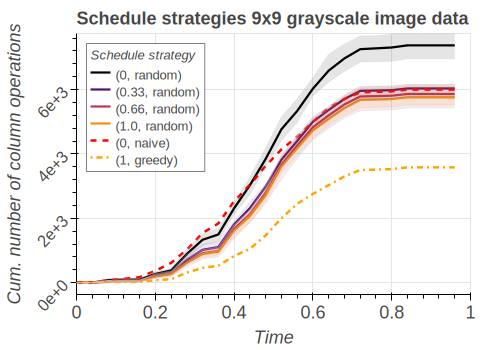
\includegraphics[width=0.48\textwidth]{varying_d.pdf}
	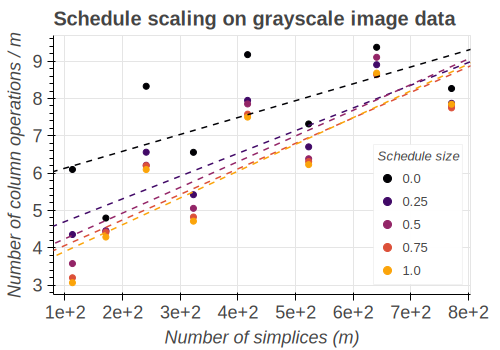
\includegraphics[width=0.48\textwidth]{varying_nd.pdf}
	\caption{Performance comparison between various scheduling strategies. On the left, the cumulative column operations required to compute the 1-parameter family is shown for varying schedule sizes ($d$) and strategies. On the right, both the size of the schedule and the data set $(m)$ are varied. }
	\label{fig:movie_perf}
\end{figure}

In the second test, we measure the asymptotics of our greedy LCS-based approach. To do this, we generated 8 video data sets again of the expanding annulus outlined in section~\ref{sec:motivation}, each of increasing grid sizes of $5 \times 5$, $6 \times 6$, $\dots$, $12 \times 12$. For each data set, we compute persistence over the duration of the video, again testing five evenly spaced settings of $\alpha \in [0,1]$---the results are shown in the right plot of Figure~\ref{fig:movie_perf}. On the vertical axis, we plot the total number of column operations needed to compute persistence across 25 evenly-spaced time points \emph{as a ratio} of the data set size ($m$); we also show the regression curves one obtains for each setting of $\alpha$. As one can see from the Figure, the cost of using the greedy heuristic tends to increase sub-linearly as a function of the data set size, suggesting the move scheduling approach is indeed quite scalable. Moreover, schedules with minimal size tended to be cheaper than otherwise, confirming our initial hypothesis that repairing the decomposition less can lead to substantial reductions at run-time.  

\subsection{Crocker stacks}
There are many challenges to characterizing topological behavior in dynamic settings. One approach is to trace out the curves constituting a continuous family of persistence diagrams in $\mathbb{R}^3$---the \emph{vineyards} approach---however this visualization can be cumbersome to work with as there are potentially many such vines tangled together, making topological critical events with low persistence difficult to detect. Moreover, the \emph{vineyards} visualization does not admit a natural simplification utilizing the stability properties of persistence, as individual vines are not stable: if two vines move near each other and then pull apart without touching, then a pairing in their corresponding persistence diagrams may cross under a small perturbation, signaling the presence of an erroneous topological critical event~\cite{topaz2015topological, xian2020capturing}. 

\begin{figure}[t]
	\centering
	\includegraphics[width=0.95\textwidth]{crocker_combo_1.png}
	\caption{A Crocker plot (right) depicts the evolution of dimension $p = 1$ Betti curves over time. The green $\mathrm{X}$ marks correspond chronologically to the complexes (left), in row-major order. The large orange and purple areas depict $1$-cycles persisting in both space (y-axis) and time (x-axis).} \label{fig:crocker1}
\end{figure}

Acknowledging this, Topaz et al.~\cite{topaz2015topological} proposed the use of a 2-dimensional summary visualization, called a \emph{crocker}\footnote{\emph{crocker} stands for ``Contour Realization Of Computed k-dimensional hole Evolution in the Rips complex.'' Although the acronym includes \emph{Rips complexes} in the name, in principle a \emph{crocker} plot could just as easily be created using other types of triangulations (e.g. \v{C}ech filtrations).} plot. 
In brief, a \emph{crocker} plot is a contour plot of a family of Betti curves. Formally, given a filtration $K = K_0 \subseteq K_1 \subseteq \dots \subseteq K_m$, a $p$-dimensional \emph{Betti curve} $\beta_p^{\bullet}$ is defined as the ordered sequence of $p$-th dimensional Betti numbers:
$$ \beta_p^\bullet = \{ \, \mathrm{rank}(H_p(K_0)), \, \mathrm{rank}(H_p(K_1)), \, \dots, \, \mathrm{rank}(H_p(K_m))\, \}$$
Given a time-varying filtration $K(\tau)$, a \emph{crocker} plot displays changes to $\beta_p^\bullet(\tau)$ as a function of $\tau$. An example of a \emph{crocker} plot generated from the simulation described below is given in Figure~\ref{fig:crocker1}. Since only the Betti numbers at each simplex in the filtration are needed to generate these Betti curves, the persistence diagram is not directly needed to generate a \emph{crocker} plot; it is sufficient to use e.g. any of the specialized methods discussed in~\ref{sec:related_work}. This dependence only on the Betti numbers makes \emph{crocker} plots easier to compute than standard persistence, however what one gains in efficiency one loses in stability; it is known that Betti curves are inherently unstable with respect to small fluctuations about the diagonal of the persistence diagram. 

Xian et al.~\cite{xian2020capturing} showed that \emph{crocker} plots may be \emph{smoothed} to inherit the stability property of persistence diagrams and reduce noise in the visualization. That is, when applied to a time-varying persistence module $M = \{M_t\}_{t \in [0, T]}$, an $\alpha$-smoothed \emph{crocker} plot for $\alpha \geq 0$ is the rank of the map $M_t(\epsilon - \alpha) \to M_t(\epsilon + \alpha)$ at time $t$ and scale $\epsilon$. For example, the standard crock plot is a $0$-smoothed \emph{crocker} plot. Allowing all three parameters ($t, \epsilon, \alpha$) to vary continuously leads to 3D visualization called an $\alpha$\emph{-smoothed crocker stack}.
\begin{definition}[crocker stack]
	A \emph{crocker stack} is a family of $\alpha$-smoothed crock plots which summarizes the topological information of a time-varying persistence module $M$ via the function $f_M : [0, T] \times [0, \infty) \times [0, \infty) \to \mathbb{N}$, where:
	$$ f_M(t,\epsilon, \alpha) = \mathrm{rank}(M_t(\epsilon - \alpha) \to M_t(\epsilon + \alpha)) $$
	and $f_M$ satisfies $f_M(t,\epsilon,\alpha') \leq f_M(t,\epsilon, \alpha)$ for all $0 \leq \alpha \leq \alpha'$.
\end{definition}
%\noindent A crocker stack is a sequence of $\alpha$-smoothed crocker plots that vary over $\alpha \geq 0$, satisfying $f_M(t,\epsilon,\alpha) \leq f_M(t,\epsilon, \alpha)$ for all $\alpha \geq \alpha'$. 
\noindent Note that, unlike \emph{crocker} plots, applying this $\alpha$ smoothing efficiently \emph{requires} the persistence pairing. Indeed, it has been shown that \emph{crocker stacks} and stacked persistence diagrams (i.e. \emph{vineyards}) are equivalent to each other in the sense that either one contains the information needed to reconstruct the other~\cite{xian2020capturing}. Thus, computing \emph{crocker stacks} reduces to computing the persistence of a (time-varying) family of filtrations.

%To describe this formally, let $K_\tau^\epsilon$ denote a simplicial filtration with simplices $\sigma \in K_\tau^\epsilon$ whose function value $f_\tau(\sigma) \leq \epsilon$. The $\alpha$

To illustrate the applicability of our method, we test the efficiency of computing these \emph{crocker stacks} using a spatio-temporal data set. Specifically, we ran a flocking simulation similar to the one run in~\cite{topaz2015topological} with $m = 20$ vertices moving around on the unit square equipped with periodic boundary conditions (i.e. $S^1 \times S^1$). We simulated movement by equipping the vertices with a simple set of rules which control how the individual vertices position change over time. Such simulations are also called \emph{boid} simulations, and they have been extensively used as models to describe how the evolution of collective behavior over time can be described by simple sets of rules.
The simulation is initialized with every vertex positioned randomly in the space; the positions of vertices over time is updated according to a set of rules related to the vertices' acceleration, distance to other vertices, etc. To get a sense of the time domain, we ran the simulation until a vertex made at least 5 rotations around the torus. 

Given this time-evolving data set, we computed the persistence diagram of the Rips filtration up to $\epsilon = 0.30$ at 60 evenly spaced time points using three approaches: the standard algorithm \texttt{pHcol} applied naively at each of the 60 time steps, the \emph{vineyards} algorithm applied to (linear) homotopy connecting filtrations adjacent in time, and our approach using \emph{moves}.   
The cumulative number of $O(m)$ column operations executed by three different approaches. Note again that \emph{vineyards} requires generating many decompositions by design (in this case, $\approx 1.8M$). The standard algorithm \texttt{pHcol} and our move strategy were computed at 60 evenly spaced time points. As depicted in Figure~\ref{fig:boid_sim_results}, our \emph{moves} strategy is far more efficient than both \emph{vineyards} and the naive \texttt{pHcol} strategies. 

\begin{figure}[ht]
	\centering
%	\includegraphics[width=0.6\textwidth, height=14.15em]{boid_sim_results.png} % arxiv only
	\includegraphics[width=\textwidth, height=16.15em]{boid_sim_results.png} % springer only
	\caption{On the left, the cumulative number of column operations (log-scale) of the three baseline approaches tested. On the right, the normalized $K_\tau$ between adjacent filtrations depicts the coarseness of the discretization---about $5\%$ of the $\approx O(m^2)$ simplex pairs between adjacent filtrations are discordant.}
	\label{fig:boid_sim_results}
\end{figure}

\subsection{Multiparameter persistence}
Given a procedure to filter a space in multiple dimensions simultaneously, a \emph{multifiltration}, the goal of multi-parameter persistence is to identify persistent features by examining the entire multifiltration. 
Such a generalization has appeared naturally in many application contexts, showing potential as a tool for exploratory data analysis~\cite{lesnick2012multidimensional}. Indeed, one of the drawbacks of persistence is its instability with respect to strong outliers, which can obscure the detection of significant topological structures~\cite{buchet2015topological}.
One exemplary use case of multi-parameter persistence is to detect these strong outliers by filtering the data with respect to both the original filter function \emph{and} density.
In this section, we show the utility of scheduling with a real-world use case: detecting the presence of a low-dimensional topological space which well-approximates the distribution of natural images. 
As a quick outline, in what follows we briefly recall the fibered barcode invariant~\ref{sec:fibered_barcode}, summarize its potential application to a particular data set with known topological structure~\ref{sec:natural_images}, and conclude with experiments of demonstrating how scheduling enables such applications~\ref{sec:empirical_klein}.   

\subsubsection{Fibered barcode}\label{sec:fibered_barcode}
Unfortunately, unlike the one-parameter case, there is no complete discrete invariant for multi-parameter persistence.
Circumventing this, Lesnick et al~\cite{lesnick2015interactive} associate a variety of incomplete invariants to 2-parameter persistence modules; we focus here on the \emph{fibered barcode} invariant, defined as follows: 
\begin{definition}[Fibered barcode]
	%\in \overline{\mathcal{L}}
	The fibered barcode $\mathcal{B}(M)$ of a 2D persistence module $M$ is the map which sends each line  $L \subset \mathbb{R}^2$ with non-negative slope to the barcode $\mathcal{B}_L(M)$: 
%	$$ L \mapsto \mathcal{B}_L(M) $$
$$ \mathcal{B}(M) = \{ \; B_L(M) : L \in \mathbb{R} \times \mathbb{R}^{+} \; \}$$
Equivalently, $\mathcal{B}(M)$ is the 2-parameter family of barcodes given by restricting $M$ to the of set affine lines with non-negative slope in $\mathbb{R}^2$. 
\end{definition} 
\noindent Although an intuitive invariant, it is not clear how one might go about computing $\mathcal{B}(M)$ efficiently. 
One obvious choice is fix $L$ via a linear combination of two filter functions, restrict $M$ to $L$, and compute the associated 1-parameter barcode. 
However, this is an $O(m^3)$ time computation, which is prohibitive for interactive data analysis purposes. 

%Lesnick and Wright~\cite{lesnick2015interactive} introduced an elegant reparameterization that not only fully characterizes $\mathcal{B}(M)$, but also yields an efficient method for rendering $\mathcal{B}_L(M)$ in real time. 
Utilizing the equivalence between the rank and fibered barcode invariants, Lesnick and Wright~\cite{lesnick2015interactive} developed an elegant way of computing $\mathcal{B}(M)$ via a re-parameterization using standard point-line duality. This clever technique effectively reduces the fibered barcode computation to a sequence of 1-D barcode computations at ``template points'' lying within the 2-cells of a particular planar subdivision $\mathcal{A}(M)$ of the half-plane $[0, \infty) \times \mathbb{R}$. This particular subdivision is induced by the arrangement of ``critical lines'' derived by the bigraded Betti numbers $\beta(M)$ of $M$.
As the barcode of one template point $\mathcal{T}_e$ at the 2-cell $e \in \mathcal{A}(M)$ may be computed efficiently by re-using information from an adjacent template point $\mathcal{T}_{e'}$,~\cite{lesnick2015interactive} observed that computing the barcodes of all such template points (and thus, $\mathcal{B}(M)$) may be reduced to ordering the 2-cells in $\mathcal{A}(M)$ along an Eulerian path traversing the dual graph of $\mathcal{A}(M)$. 
The full algorithm is out of scope for this effort; we include supplementary details for the curious reader in the appendix~\ref{app:2d_pers}. 
\\
\\
\noindent 
\textbf{Example 4.1}: Consider a small set of noisy points distributed around $S^1$ containing a few strong outliers, as shown on the left side of Figure~\ref{fig:bifiltration_ex2}. Filtering this data set with respect to the Rips parameter and the complement of a kernel density estimate yields a bifiltration whose various invariants are shown in the middle figure. The gray areas indicate homology with positive dimension---the lighter gray area $\mathrm{dim}_1(M) = 1$ indicates a persistent loop was detected.
On the right side, dual space is shown: the black lines are the critical lines that form $\mathcal{A}(M)$, the blue dashed-lines the edges of the dual graph of $\mathcal{A}(M)$, the rainbow lines overlaying the dashed-lines form the Eulerian path, and the orange barycentric points along the 2-cells of $\mathcal{A}(M)$ represent where the barcodes templates $\mathcal{T}_e$ are parameterized. 
\begin{figure}[t]
	\includegraphics[width=0.98\textwidth]{bifiltration_ex2}
	\caption{Bipersistence example on an $8 \times 8$ coarsened grid. On the left, the data, colored by density. In the middle, the bigraded Betti numbers $\beta_0(M)$ and $\beta_1(M)$ (green and red, resp.), the dimension function (gray), and a line $L$ emphasizing the persistence of features with high density. On the right, the line arrangement $\mathcal{A}(M)$ lying in the dual space derived from the $\beta(M)$. }
	\label{fig:bifiltration_ex2}
\end{figure}
%The shortest path $\Gamma^\ast$ spanning the vertices of $G$ is shown by the solid rainbow colored lines, with the traversal beginning in the top-left cell (at the red edge) and ending at the bottom-right cell (the indigo edge). Traversing $\Gamma^\ast$ can be done via a simple depth-first search, though note that a $R=DV$ decomposition needs to be stored at each degree-3 or higher vertex in $\Gamma^\ast$ to avoid redundant computations as the traversal recurses. 
\\

Despite its elegance, there are significant computational barriers prohibiting the 2-parameter persistence algorithm from being practical. 
An analysis from~\cite{lesnick2015interactive} (using \emph{vineyards}) shows the barcodes template computation requires on the order of $O(m^3 \kappa + m \kappa^2 \log \kappa)$ elementary operations and $O(m \kappa^2)$ storage, where $\kappa$ is a coarseness parameter.
Since the number of 2-cells in $\mathcal{A}(M)$ is on the order $O(\kappa^2)$, and $\kappa$ itself is on the order of $O(m^2)$ in the worst case, the scaling of the barcode template computation may approach $\approx O(m^5)$---this is both the highest complexity and most time-intensive sub-procedure the RIVET software~\cite{rivet} depends on. 
Despite this significant complexity barrier, in practice the external stability result from~\cite{landi2014rank} justifies the use of a grid-like reduction procedure which approximates the module $M$ with a smaller module $M'$, enabling practitioners to restrict the size of $\kappa$ to a relatively small constant. 
This in-turn dramatically reduces the size of $\mathcal{A}(M)$ and thus the number of barcode templates to compute. 
Moreover, the ordering of barcode templates given by the dual graph traversal implies that adjacent  template points should be relatively close---so long as $\kappa$ is not too small---suggesting adjacent templates may productively share computations due to the high similarity of their associated filtrations. 
%Intuitively, similar barcode templates should be easier to compute in sequence than independently. 
Indeed, as algorithm~\ref{alg:schedule} was designed for precisely such a computation, 2-parameter persistence is prototypical of the class of methods that stand to benefit from \emph{moves}. 

 \subsubsection{Natural images dataset}\label{sec:natural_images}
A common hypothesis is that high dimensional data tend to lie in the vicinity of an embedded, low dimensional manifold or topological space. An exemplary demonstration of this is given in the analysis by Lee et al.~\cite{lee2003nonlinear}, who explored the space of high-contrast patches extracted from Hans van Hateren's~\cite{hateren_schaaf_1998} still image collection\footnote{See \url{http://bethgelab.org/datasets/vanhateren/} for details on the image collection.}, which consists of $\approx 4,000$ monochrome images depicting various areas outside Groningen (Holland). 
In particular,~\cite{lee2003nonlinear} were interested in exploring how high-contrast $3 \times 3$ image patches  were distributed, in pixel-space, with respect to predicted spaces and manifolds.
Formally, they measured contrast using a discrete version of the scale-invariant Dirichlet semi-norm:
$$ \lVert x \rVert_D = \sqrt{\sum_{i \sim j}(x_i - x_j)^2} = \sqrt{x^T D x}$$
where $D$ is a fixed matrix whose quadratic form $x^T D x$ applied to an image $x \in \mathbb{R}^9$ is proportional to the sum of the differences between each pixels 4 connected neighbors (given above by the relation $i \sim j$).
Their research was primarily motivated by discerning whether there existed clear qualitative differences in the distributions of patches extracted from images of different modalities, such as optical and range images.
By mean-centering, contrast normalizing, and``whitening'' the data via the Discrete Cosine Transform (DCT), they show a convenient basis for $D$ may be obtained via an expansion of 8 certain non-constant eigenvectors, shown below: 
%\vspace{-0.2em}
\begin{center}
	\includegraphics[width=0.80\textwidth]{dct_basis} 
\end{center}
%\begin{figure}[h]
%	\captionsetup{labelformat=empty}
%	\centering
%	\includegraphics[width=0.90\textwidth]{dct_basis}
%	\caption{}
%\end{figure}
%\vspace{-1.5em}
Since these images are scale-invariant, the expansion of these basis vectors spans the 7-sphere, $S^7 \subset \mathbb{R}^8$. Using a Voronoi cell decomposition of the data, their distribution analysis suggested that the majority of data points concentrated in a few high-density regions. 

In follow-up work, Carlsson et al.~\cite{carlsson2008local} found---using persistent homology---that the distribution of high-contrast $3 \times 3$ patches is actually well-approximated by a Klein bottle $\mathcal{M}$---around 60\% of the high-contrast patches from the still image data set lie within a small neighborhood around $\mathcal{M}$ accounting for only 21\% of the 7-sphere's volume. 
Along a similar vein, Perea~\cite{perea2014klein} established a dictionary learning framework for efficiently estimating the distribution of patches from texture images, prompting applications for persistent homology in sparse coding contexts. 

 \begin{figure}[t]
	\includegraphics[width=0.98\textwidth]{natural_images}
	\caption{Bipersistence example of natural images data set on a $12 \times 16$ coarsened grid. On the left, a projection of the full data set is shown, along with the 15 landmark patches. (Middle) the bigraded Betti numbers and a fixed line $L$ over parameter space. 
	As before, the $0/1/2$ dimension bigraded Betti numbers are shown in green/red/yellow, respectively, with the blue region highlighting where $\mathrm{dim}(M) = 5$. (Right) five persistent features representing $B_L(M)$ are revealed from the middle, matching $\beta_1$ of the three-circle model. }
	\label{fig:patch_data_dgm}
\end{figure}

If one was not aware of the analysis done by~\cite{lee2003nonlinear, hateren_schaaf_1998, carlsson2008local, perea2014klein}, it is not immediately clear a priori that the Klein bottle model is  a good candidate for capturing the non-linearity of image patches. 
Indeed, armed with a refined topological intuition, Carlsson still needed to perform extensive sampling, preprocessing, and model fitting techniques in order to reveal the underlying topological space with persistent homology~\cite{carlsson2008local}.
One reason such preprocessing is needed is due to persistent homology's aforementioned instability with respect to strong outliers. 
In the ideal setting, a multi-parameter approach that accounts for the local density of points should require far less experimentation. 
%Nonetheless, given a suitable treatment of strong outliers using by e.g. filtering both on the geometry and the density of the image patches, the homology of the Klein bottle should become apparent through a persistence computation.
%Nonetheless, as we have mentioned, among the first uses of persistent homology was the so-called ``homology inference problem''~\cite{perea2018brief}; given a suitable treatment of strong outliers using by e.g. filtering both on the geometry and the density of the image patches, the homology of the Klein bottle should become apparent through a persistence computation.
 
To demonstrate the benefit of 2-parameter persistence on the patch data, consider the (coarsened) fibered barcode computed from a standard Rips / codensity bifiltration on a representative sample of the image data from~\cite{hateren_schaaf_1998}, shown in Figure~\ref{fig:patch_data_dgm}. 
From the bigraded Betti number and the dimension function, one finds that a large area of the dimension function is constant (highlighted as the blue portion in the middle of Figure~\ref{fig:patch_data_dgm}), wherein the first Betti number is 5. Further inspection suggests one plausible candidate is the three-circle model $C_3$, which consists of three circles, two of which (say, $S_v$ and $S_h$) intersect the third (say, $S_\mathrm{lin}$) in exactly two points, but themselves do not intersect. 
Projecting the image data onto the first two basis vectors from the DCT shown above leads to the projection shown in the top left of Figure~\ref{fig:patch_data_dgm}, of which 15 landmark points are also shown. Observe the data are distributed well around three ``circles''---the outside circle capturing the rotation gradient of the image patches ($S_{\mathrm{lin}}$), and the other two capturing the vertical and horizontal gradients ($S_v$ and $S_h$, respectively). Since the three circle model is the 1-skeleton of the Klein bottle, one may concur with Carlssons analysis~\cite{carlsson2008local} that the Klein bottle may be a reasonable candidate upon which the image data are distributed. 
% This can be further verified empirically by e.g. using the iterative, meanshift-like procedure described in~\cite{carlsson2008local} to fit a parameterization of the model in question to the data. 

The degree to which multi-parameter persistence simplifies this exploratory phase cannot be understated: we believe multi-parameter persistence has a larger role to play in manifold learning. 
Unfortunately, as mentioned prior, the compute barriers effectively bar its use in practice. 

\subsubsection{Accelerating 2D persistence}\label{sec:empirical_klein}
%As we have outlined the computational theory of 2-parameter persistence and elucidated its relevance to our proposed move scheduling approach, 
Having outlined the computational theory of 2-parameter persistence, we now demonstrate the efficiency of \emph{moves} using the same high-contrast patch data set studied in~\cite{lee2003nonlinear} by evaluating the performance of various methods at computing the fibered barcode invariant via the parameterization from~\ref{sec:fibered_barcode_reparam}. 

Due to the aforementioned high complexity of the fibered barcode computation, we begin by working with a subset of the image patch data $\mathcal{X}$. 
We combine the use of furthest-point sampling and proportionate allocation (stratified) sampling to sample landmarks $X \subset \mathcal{X}$ distributed within $n = 25$ strata. Each stratum consists of the $(1/n)$-thick level set given the $k$-nearest neighbor density estimator $\rho_{15}$ with $k = 15$. The use of furthest-point sampling gives us certain coverage guarantees that the geometry is approximately preserved within each level set, whereas the stratification ensures the original density of is approximated preserved as well. 
From this data set, we construct a Rips-(co)density bifiltration using $\rho_{15}$ equipped with the geodesic metric computed over the same k-nearest neighbor graph on $X$. 
Finally, we record the number of column reductions needed to compute the fibered barcode at a variety of levels of coarsening using $\mathtt{pHcol}$, \emph{vineyards}, and our \emph{moves} approach. The results are summarized in Table~\ref{tab:barcode_templates}. We also record the number of 2-cells in $\mathcal{A}(M)$ and the number of permutations applied encountered along the traversal of the dual graph for both \emph{vineyards} and \emph{moves}, denoted in the table as $d_K$ and $d_{\mathrm{LCS}}$, respectively. 
%Specifically, we begin by extracting a representative subset of the set $X \subset \mathcal{X}$ of patches representing the top 30\% densest patches of the space of all patches $\mathcal{X}$, where the notion of density is approximated with a k-nearest neighbor (knn) density estimator $\rho$. Carlsson et al.~\cite{carlsson2008local} studied a variety of choices of $k$ in order to understand how localized the data were distributed around the Klein bottle model. He determined empirically that when $k \approx 15$, the top 30\% captures three types of directional shifts in the grayscale gradients of the image patches. These three gradients were shown to be captured well by the three-circle model $C_3$---the 1-skeleton of the Klein bottle.  One of the circles, $S_{\mathrm{lin}}$, parameterizes a the rotational gradient, whereas the other two $S_v$ and $S_h$ parameterize vertical and horizontal gradients.  
%It was shown in~\cite{carlsson2008local} that when $k \approx 300$, the top 30\% of data extracted from the knn density estimator $\rho_{300}$ `fills out' the two-manifold, yielding Betti numbers $\beta_0 = \beta_1 = 1$, whereas when $k$ is decreases to a more localized estimate, the three-circle model is recovered, which has Betti numbers $\beta_0 = 1, \beta_1 = 5$.
%In theory, this bifiltration should be well approximated by the $C_3$ model, which one ought to be able to determine by a careful inspection of the fibered barcode. That is, since $C_3$ has $\beta_1  = 5$, there should be some line $L$ which induces a 1-parameter filtration whose corresponding persistence diagram (for dimension $1$) displays five highly persistent features. We show an example of the data, the bigraded Betti numbers, and the persistence diagram extracted from a particular choice of line $L$ in Figure~\ref{fig:patch_data_dgm}. 
%The example from~\ref{fig:patch_data_dgm} demonstrates a practical application of the fiber barcode  to uncovering the underlying topological structure characterizing a ``real-world'' data set. Indeed, this is just one of the many applications of multidimensional persistence. As discussed, one of the main issues inhibiting the use of rank invariant in practice is computation. In Table~\ref{tab:barcode_templates}, we record a variety of statistics related to the computation of the rank invariant on the bifiltration constructed from the natural images data set. 
%TODO: finish explanation
%An increasingly refined 
\begin{table}[h]
\caption{Cost to computing $\mathcal{T}$ for various coarsening choices of $\beta(M)$.}\label{tab:barcode_templates}
\centering
\begin{tabular}{ m{1.6cm} m{1.6cm} m{1.2cm} m{2.8cm} m{2.4cm} }
 \hline
 %\multicolumn{7}{|c|}{ Size and cost of constructing $\mathcal{A}^\ast(M)$ } \\
 %\hline
  \multicolumn{1}{|c|}{ $\beta(M)$ } & \multicolumn{1}{|c|}{$\mathcal{A}(M)$ } & \multicolumn{3}{c|}{ Col. Reductions / Permutations } \\
 \hline
\small{Coarsening} & \# 2-cells & \texttt{phCol} & Vineyards / $d_{K}$ & Moves / $d_{\text{LCS}}$ \\
 \hline
 8 x 8 & 39 & 94.9K & 245K / 1.53M & 38.0K / 11.6K   \\
 \hline
 12 x 12 & 127 & 318K & 439K / 2.66M & 81.9K / 33.0K \\
 \hline 
 16 x 16 & 425 & 1.07M & 825K / 4.75M & 114K / 87.4K \\
 \hline 
  20 x 20 & 926 & 2.32M & 1.15M / 6.77M  & 148K / 154K\\
 \hline 
  24 x 24 & 1.53K & 3.92M & 1.50M / 8.70M & 184K / 232K  \\
   \hline
 \end{tabular}
\label{table:dual_graph_costs}
\end{table}  

As shown on the table, when the coarsening $\kappa$ is small enough, we're able to achieve a significant reduction in the number of total column operations needed to compute $\mathcal{T}$ compared to both \emph{vineyards} and $\mathtt{pHcol}$. %though it's worth noting that permutations are constant time for vineyards while they require at most $O(m)$ elementary operations for moves. 
This is further reinforced by the observation that \emph{vineyards} is particularly inefficient when then 1-parameter family is coarse. Indeed, \emph{moves} requires about 3x less column operations than naively computing $\mathcal{T}$ independently. However, note that as the coarsening becomes more refined and more 2-cells are added to $\mathcal{A}(M)$, \emph{vineyards} becomes a more viable option compared to $\mathtt{pHcol}$---as the asymptotics suggests---though even at the highest coarsening we tested the gain in efficiency is relatively small. In contrast, \emph{moves} scales quite well with this refinement, requiring about $12\%$  and $\approx 5\%$ of the number of column operations as \emph{vineyards} and $\mathtt{pHcol}$, respectively. 


%[1,]         8   94945  245297  37999
%[2,]        12  318828  438932  81894
%[3,]        16 1073995  824639 114005
%[4,]        20 2328432 1153742 148434
%[5,]        24 3916177 1506480 184125

% permutations  (b, vineyards, moves) 
% 8, 1525826, 11677
% 12, 2657899, 33056
% 16, 4749576, 87417
% 20, 6772406, 154029
% 24, 8697797, 231603

%To obtain family of filtrations, we computed the Rips filtration up to a fixed $\epsilon = 0.20$ at $d = 150$ snapshots in time. The simulation length is normalized such that the duration of the entire simulation is $1$ unit.  Each time point is evenly sampled between $[0,1]$, and 
%simulated 
%We tested our approach against a variety of different methods.
%\begin{figure}[ht]
%	\includegraphics[width=0.95\textwidth, height=2.5in]{prelim_results}
%	\caption{[Placeholder] 	Cumulative number of $O(m)$ operations (left, middle), and the distribution of $K_\tau$ distances between each adjacent permutation (right). The left plot shows the cumulative number of column operations (in log-scale) for various strategies, and the middle plot shows the cumulative number of permutations.}
%	\label{fig:res1}
%\end{figure}


\section{Conclusion and Future Work}\label{sec:conclusion}
In conclusion, we presented a scheduling algorithm for efficiently updating a decomposition in coarse dynamic settings. Our approach is simple, relatively easy to implement, and fully general: it does not depend on the geometry of underlying space, the choice of triangulation, or the choice of homology dimension. Moreover, we supplied efficient algorithms for our scheduling strategy, provided tight bounds where applicable, and demonstrated our algorithms performance with several real world use cases.

There are many possible applications of our work beyond the ones discussed in section~\ref{sec:results}, such as e.g. accelerating PH featurization methods or detecting homological critical points in dynamic settings.
%\begin{enumerate}
%	\item Accelerating PH featurization methods for time-varying systems 
%	\item Optimization procedures involving persistence diagrams
%	\item Detecting homological critical points in time-varying filtrations
%\end{enumerate}
Indeed, we see our approach as potentially useful to any situation where the structure of interest can be cast as a parameterized family of persistence diagrams. Areas of particular interest include time-series analysis and dynamic metric spaces~\cite{kim2020spatiotemporal}. 

The simple and combinatorial nature of our approach does pose some limitations to its applicability. For example, better bounds or algorithms may be obtainable if stronger assumptions can be made on how the filtration is changing with time. Moreover, if the filtration $(K, f)$ shares little similarity to the ``target'' filtration $(L,f')$, then the overhead of reducing the simplices from $L \setminus K$ appended to the decomposition derived from $K$ may be large enough to motivate simply computing the decomposition at $L$ independently. 
Our approach is primarily useful if the filtrations in the parameterized family are ``nearby'' in the combinatorial sense. 

From an implementation perspective, one non-trivial complication of our approach is its heavy dependence on a particular sparse matrix data structure, which permits permuting both the row and columns of a given matrix in at most $O(m)$ time~\cite{cohen2006vines}. As shown with the natural images example in section~\ref{sec:results}, there are often more permutation operations being applied than there are column reductions. In the more standard \emph{compressed} sparse matrix representations,
%\footnote{By ``standard,'' we mean any of the common sparse representations used in scientific computing packages, like SciPy's sparse module (\url{https://docs.scipy.org/doc/scipy/reference/sparse.html})}, 
permuting both the rows and columns generally takes at most $O(Z)$ time, where $Z$ is the number of non-zero entries, which can be quite expensive if the particular filtration has many cycles. As a result, the more complex sparse matrix representation from~\cite{cohen2006vines} is necessary to be efficient in practice. 

Moving forward, our results suggest there are many aspects of computing persistence in dynamic settings yet to be explored. 
For example, it's not immediately clear whether one could adopt, for example, the twist optimization~\cite{chen2011persistent} used in the reduction algorithm to the dynamic setting. Another direction to explore would be the analysis of our approach under the cohomology computation~\cite{de2011dualities}, or the specialization of the move operations to specific types of filtrations such as Rips filtrations. Such adaptations may result in even greater reductions in the number of column operations, as have been observed in practice for the standard reduction algorithm~\cite{bauer2021ripser}. 
Moreover, though we have carefully constructed an efficient greedy heuristic in section~\ref{sec:proxy_objective} and illustrated a different perspective with which to view our heuristic (via crossing minimization), it is an open question whether there exists a more structured reduction of~\eqref{eq:schedule_cost} or~\eqref{eq:sorting_additive} to a better-known problem. 


\section{Declarations}
 
\textbf{Ethical Approval:} Not applicable.
\\
\\
\noindent \textbf{Competing interests:} 
The authors declare that they have no competing interests that could influence the interpretation or presentation of the research findings. There are no financial or personal relationships with individuals or organizations that could bias the outcomes of this work.
\\
\\
\noindent
\textbf{Authors' contributions:}
The contributions of each author to this article were as follows:
\begin{enumerate}
	\item Matt Piekenbrock: conceptualization, methodology design, algorithm development, experimental design \& analysis, software development. 
	\item Jose Perea: Conceptualization, methodology design, literature review, critical revision of the manuscript, final approval of the version to be published.
\end{enumerate}
All authors have reviewed and approved the final version of the manuscript and have agreed to be accountable for all aspects of the work.
\\
\\
\noindent 
\textbf{Funding:}
The research presented in this work is partially supported by the National Science Foundation through grants CCF-2006661 and CAREER award DMS-1943758. The funding source had no role in the study design, data collection and analysis, decision to publish, or preparation of the manuscript.
\\
\\
\noindent \textbf{Availability of data and materials:} Links to the software and data used for the experiments can be found at: \url{https://github.com/peekxc/move_schedules}.

% REQUIRED: siamplain format
% Looks like you have to just not specify the style with springer 
 \bibliographystyle{siamplain} % springer only 
%\bibliographystyle{unsrt}
% \bibliographystyle{plain} % arxiv only
\bibliography{move_schedules}

\newpage 
\appendix
\section{Appendix}

\subsection{Algorithms}\label{app:algorithms}

\textbf{Reduction Algorithm: } The reduction algorithm, outlined in pseudocode in Algorithm~\ref{alg:reduce}, is the most widely used modality for computing persistence. While there exists other algorithms for computing persistence, they are typically not competitive with the reduction algorithm in practice. 
\begin{algorithm}[h!]
	\setstretch{1.15}
	\caption{Reduction Algorithm (\texttt{pHcol}) }
	\begin{algorithmic}[1]
		\Require{$D = (m \times m)$ filtration boundary matrix }
		\Ensure{$R$ is reduced, $V$ is full rank upper triangular, and $R = D V$}
		\Function{Reduction}{$D$}
		\State $(R, V) \gets (D, I)$
		\For{$j = 1$ \textbf{to} $m$} 
			\While{$\exists \, i < j$ \textbf{such that} $\mathrm{low}_R(i) = \mathrm{low}_R(j)$ }
				\State $\lambda \gets \mathrm{pivot}_R(j)/\mathrm{pivot}_R(i)$
				\State $(\mathrm{col}_R(j), \mathrm{col}_V(j)) \mathrel{-}= \left ( \lambda \cdot \mathrm{col}_R(i), \lambda \cdot \mathrm{col}_V(i) \right )$
			\EndWhile
		\EndFor 
		\State \Return $(R, V)$
		\EndFunction
	\end{algorithmic}	\label{alg:reduce}
\end{algorithm}
The algorithm begins by copying $D$ to a new matrix $R$, to be subsequently modified in-place. After  $V$ is set to the identity, the algorithm proceeds with column operations on both $R$ and $V$, left to right, until the decomposition invariants are satisfied. Since each column operation takes $O(m)$ and there are potentially $O(k)$ columns in $D$ with identical low entries (line 4 in ~\ref{alg:reduce}, observe that the reduction algorithm below clearly takes $O(m^2 k)$ time. Since there exist complexes where $k \sim O(m)$, one concludes the bound of $O(m^3)$ is tight~\cite{morozov2005persistence}, though this seems to only be true on pathological inputs. A more refined analysis by Edelsbrunner et al.~\cite{edelsbrunner2000topological} shows the reduction algorithm scales by the sum of squares of the cycle persistences. 
%\\
%\\
%\noindent \textbf{Move Left:}
%We recall an important claim given in~\cite{busaryev2010tracking} on the effect that move operations have on the status of simplices in the pairing. Recall from section~\ref{sec:background} that simplices which create new homology classes are called \emph{creators} and simplices that destroy homology classes are called \emph{destroyers}.
%%\begin{proposition}[Locality of moves~\cite{busaryev2010tracking}]
%%	Other than the simplex $\sigma_i$ being moved, $\mathrm{MoveRight}(i,j)$ cannot change a destroyer to a creator, $\mathrm{MoveLeft}(i,j)$ cannot change a creator to destroyer, and neither move operation changes the status of any simplex in $K$ outside of the interval $[i,j]$.  
%%\end{proposition}
%\noindent The effect of the movement on intermediate simplices depends on the direction of the movement. If $i < j$ (respectively, $j < i$), all simplices at positions $k \in [i+1\;:\;j] $ are shifted down (respectively, up) by $1$. 
%\subsubsection{LCS-Sort}
\\
\\
\noindent \textbf{LCS-Sort:}
The algorithm to construct a schedule from a given LIS is simple enough to derive using the rules discussed in section~\ref{sec:schedule_construction} (namely, equation~\eqref{eq:valid_move}, but nonetheless for posterity’s sake we record it here for the curious reader; the pseudocode is given in Algorithm~\ref{alg:sorting}.

The high level idea of the algorithm is to first construct the LCS between two permutations $p,q \in S_m$ and then apply cyclic permutations successively to $p$, each step adding a new element extending the LCS. 
The algorithmic steps are as follows: first, one re-labels $q \mapsto \iota$ to the identity permutation $\iota = [m]$ and applies a consistent re-labeling $p \mapsto \bar{p}$. This relabeling preserves the LCS distance and has the additional advantage that $\bar{q} = \iota = [m]$ is a strictly increasing subsequence, and thus computing the LCS between $p,q \in S_m$ reduces to computing the LIS $\mathcal{L}$ of $\bar{p}$. 
Given $\mathcal{L}$ computed from $\bar{p}$, since $\mathcal{L}$ is strictly increasing, the only elements left to permute are in $\mathcal{L} \setminus \bar{p}$, which we denote with $\mathcal{D}$.
After choosing any $\sigma \in \mathcal{D}$, one applies a cyclic permutation to $\bar{p}$ that moves $\sigma$ to any position that increases the size of $\mathcal{L}$, continuing this way until the identity sequence $\iota$ is recovered.  
By sorting $\bar{p} \mapsto \iota$ by operations that (strictly) increase the size of $\mathcal{L}$, we ensure that the size of the corresponding schedule is exactly $m - \lvert \mathcal{L} \rvert$. 
  \begin{algorithm}[h!]
	\caption{Schedule construction algorithm}\label{alg:sorting}
	\setstretch{1.05}
    \begin{algorithmic}[1]
    	\Require Fixed $\bar{p} \in S_m$, LIS $\mathcal{L}$ of $\bar{p}$, and heuristic $h$
    	\Ensure $[m] = s_d \circ s_{d-1} \circ \dots \circ s_1 \circ \bar{p}$ for output sequence $\mathcal{S} = (s_i)_{i=1}^d$,
    	%set data structure $\mathcal{T}$ from section~\ref{sec:schedule_construction}
    	\Function{Schedule}{$\bar{p}$, $\mathcal{L}$, $h = \texttt{greedy}$} \Comment{See~\ref{sec:greedy} for heuristic discussion}
%    		\State $\bar{p} \gets q^{-1} \circ p$
%    		\State $\mathcal{L} \gets \mathrm{LCS}(p,q) = \mathrm{LIS}(\bar{p})$ \Comment{$O(m\log \log m)$}
    		\State $(\, \mathcal{S}, \, \mathcal{D} \,  )\gets (\, \emptyset, \, [m] \setminus \mathcal{L} \,)$
    		\While{$\mathcal{D}$\text{ is not empty }}
    		    \State Select an element $k \in \mathcal{D}$ using heuristic $h$ \Comment{e.g. equation~\eqref{eq:greedy_step}}   		        	
%    		    \State $\mathcal{T}_{\mathrm{pred}}(k) \gets \max \{ \ell \in \mathcal{L} \mid \ell \leq k \}$ 
				\State $\mathrm{k}_{\text{pred}} \gets \max \{ \ell \in \mathcal{L} \mid \ell \leq k \}$\Comment{$O(\log \log m)$ using $\mathcal{U}$}
				\State $\mathrm{k}_{\text{succ}} \gets \min \{ \ell \in \mathcal{L} \mid \ell \geq k \}$  \Comment{$O(\log \log m)$ using $\mathcal{U}$}
    		    %\text{arbitrary element in }
    		    %\State $\tau, \rho \gets \mathcal{T}_p(\sigma), \mathcal{T}_n(\sigma)$
    		    %\State $i, i_p, i_n \gets \mathcal{I}_p(\sigma), \, \mathcal{I}_p(T_{\mathrm{pred}}(\sigma)), \, \mathcal{I}_p(T_{\mathrm{succ}}(\sigma))$
    		    \State $(\,i, \,i_p, \, i_n \,) \gets ( \, \bar{p}^{-1}(k), \, \bar{p}^{-1}(\mathrm{k}_{\text{pred}}), \, \bar{p}^{-1}(\mathrm{k}_{\text{succ}} ) \, )$ \Comment{$O(1)$}
    		    %    		    \If{ $p_{\sigma} < p_{\tau}$ }
%	    		    \State $j \gets \text{arbitrary element in } [\, p_{\tau}, \, p_{\rho})$
%    		    \Else{ $p_{\rho} < p_{\sigma}$}
%    		    	\State $j \gets \text{arbitrary element in } (\, p_{\tau}, \, p_{\rho}]$
%    		    \EndIf
%				\IfThenElse{$i < i_p$}{$[\, i_p, \, i_n)$}{$(\, i_p, \, i_n]$}
				\State $j \gets \text{arbitrary } j \in [\, i_p, \, i_n)$ \textbf{if} $i < i_p$ \textbf{else} $j \in (\, i_p, \, i_n]$ \Comment{$O(1)$}
				% $\text{Pick } j \in [\, i_p, \, i_n)$ \If{ $i < i_p$ } \Else $(\, i_p, \, i_n]$ \EndIf
%    		    \If{ $i < i_p$ } 
%    		    	\State $j \gets \text{arbitrary element in } [\, i_p, \, i_n)$
%    		    \Else{ $i_n < i$ }
%	    		    \State $j \gets \text{arbitrary element in } (\, i_p, \, i_n]$ 
%    		    \EndIf
    		    \State $(\, \mathcal{S}, \mathcal{D}, \mathcal{L} \,) \gets (\, \mathcal{S} \cup (i, \, j), \, \mathcal{D} \setminus k, \, \mathcal{L} \cup k \, )$\Comment{$O(\log \log m)$}
    		    % \State $p, p^{-1} \gets m_{ij} \circ p, p^{-1} \circ m_{ij}^{-1}$
    		    \State $\bar{p}^{-1} \gets \bar{p}^{-1} \circ m_{ij}^{-1}$ where $m_{ij}$ is given by~\eqref{eq:move_perm}\Comment{$O(m)$}
    		 \EndWhile
    		 \State \Return{$\mathcal{S}$}
    	\EndFunction
	\end{algorithmic}
\end{algorithm}

To build the schedule of permutations efficiently, we use a set-like data structure $\mathcal{U}$ that supports efficient querying the successor and predecessor of any given $s \in \bar{p}$ with respect to $\mathcal{L}$ (such as a vEB tree). 
The simplified pseudocode also uses the inverse permutation $\bar{p}$ to query the position of a given element $\sigma \in \bar{p}$, although a more efficient representation can be used via an implicit treap of the \emph{displacements} array; see Section~\ref{sec:proxy_objective}.
After $\sigma$ is inserted into $\mathcal{L}$, we update $\bar{p}$, its inverse permutations $\bar{p}^{-1}$, $\mathcal{D}$ and $\mathcal{U}$ prior to the next move. The final set of permutations to sort $\bar{p} \to \iota$ (or equivalently, $p \mapsto q$) are stored in an array $\mathcal{S}$, which is then returned for further use. 

\subsection{Greedy Counter Example}\label{sec:greedy_counter_ex}
In this section we give a simple counter-example showing that the strategy that greedily chooses valid move permutations $\{ m_{ij} \}$ minimizing the quantity
\begin{equation*}
%\lvert \mathbb{I}\rvert  + \lvert \mathbb{J} \rvert
\mathrm{cost}_{RV}(m_{ij}) = \sum\limits_{l=i+1}^j \mathds{1}\left(\, v_l(i) \neq 0 \, \right) + \sum\limits_{l=1}^m \mathds{1}\left(\, \mathrm{low}_R(l) \in [i,j] \text{ and } r_l(i) \neq 0 \, \right)
\end{equation*}
can lead to arbitrarily bad behavior. A pair of filtrations is given below, each comprising the $1$-skeleton of a $3$-simplex. Relabeling $(K, f)$ to the index set $f : K \to [m]$ and modifying $(K, f')$ accordingly yields the permutations: 
%$$ K_0 = \{ {\color{red} (1) (2) (3) (4) (1,4) (2,4) (3,4) } (1,2) (2,3) (1,3) \} $$ 
%$$ K_1 = \{ {\color{red} (1) (2) (3) (4) } (1,2) (2,3) (1,3) {\color{red} (1,4) (2,4) (3,4) }\} $$ 
$$ (K, f) = \{ {\color{red} a \; b \; c \; d \; u \; v \; w} \; x \; y \; z  \} = { {\color{red} 1 \; 2 \; 3 \; 4 \; 5 \; 6 \; 7 } \; 8 \; 9 \; 10 } $$
$$ (K, f') = \{ {\color{red} a \; b \; c \; d } \; x \; y \; z \; {\color{red} u \; v \; w } \}  = { {\color{red} 1 \; 2 \; 3 \; 4 } \;8 \; 9 \; 10 \; {\color{red} 5 \; 6 \; 7 } }$$
The values colored in red corresponds to $\mathrm{LCS}(f, f')$. For this example, the edit distance is 
$d = m - \lvert \mathrm{LCS}(f, f') \rvert$ implies exactly $3$ moves are needed to map $f \mapsto f'$. There are six possible valid schedules of moves: 
\begin{alignat*}{3}
	S_1 = m_{x u}, m_{y u}, m_{z u} \quad & S_3 = m_{y u}, m_{x y}, m_{z u} \quad  & S_5 = m_{z u}, m_{x z}, m_{y z} \\
	S_2 = m_{x u}, m_{z u}, m_{y z} \quad  & S_4 = m_{y u}, m_{z u}, m_{x y} \quad  & S_6 = m_{z u}, m_{y z}, m_{x z} 
\end{alignat*}
where the notation $m_{x y}$ represents the move permutation that moves $x$ to the position of $y$. The cost of each move operation and each schedule is recorded in Table~\ref{table:move_costs}.
\begin{table}[h]
\caption{Move schedule costs}
\centering
\begin{tabular}{ m{0.4cm} m{0.8cm} m{0.8cm} m{0.8cm} m{0.8cm}  }
 \hline
 \multicolumn{5}{c}{Cost of each permutation} \\
 \hline
 & 1st & 2nd & 3rd & Total\\
 \hline
 $S_1$ & 2 & 3 & 1 & 6 \\
 \hline 
 $S_2$ & 2 & 2 & 4 & 8 \\
  \hline 
 $S_3$ & 4 & 2 & 2 & 8 \\
  \hline 
 $S_4$ & 4 & 3 & 3 & 10 \\
  \hline 
 $S_5$ & 2 & 2 & 4 & 8  \\
  \hline 
 $S_6$ & 2 & 5 & 3 & 10\\
 \hline
\end{tabular}
\label{table:move_costs}
\end{table}
Note the greedy strategy which always selects the cheapest move in succession would begin by moving $x$ or $z$ first, since these are the cheapest moves available, which implies one of $S_1, S_2, S_5, S_6$ would be picked on the first iteration. While the cheapest schedule $S_1$ is in this candidate set, an iterative greedy procedure would pick either $S_2$ or $S_5$, depending on the tie-breaker---thus, a greedy approach picking the lowest-cost move may not yield an optimal schedule. 
	Indeed, as the most expensive schedule $S_6$ is in initial iterations candidate set, we see that a greedy-procedure with an arbitrary tie-breaker could potentially yield a \emph{maximal-cost} schedule.  

\subsection{Crossing minimization}\label{sec:cross_minimization}
Conceptually, one way to view~\eqref{eq:upper_bound_move_cost} is as a crossing minimization problem over a set of $k-1$ bipartite graphs. To see this, consider two permutations: $p$ and $m_{ij} \circ p$, where $m_{ij}$ is a move permutation. 
Drawing $(p, m_{ij} \circ p)$ as a bipartite graph $(U, V, E)$, observe that there are $\lvert i - j \rvert$ edge crossings in the graph, and thus minimizing ~\eqref{eq:upper_bound_move_cost} is akin to a  structured variation of the $k$-layered crossing minimization problem. This is shown in an example below.
\\
\\
\textbf{Example}: Let  $p= (1\;2\;3\;4\;5\;6\;7\;8\;9)$ and $q = (9\;4\;2\;7\;1\;8\;6\;3\;5)$.
An example of three possible schedules, $S_1$, $S_2$, and $S_3$ sorting $p$ into $q$ is given in the figure below. 
%Each schedule, from left to right, has $21$, $31$, and $35$ crossings, respectively. 
\begin{figure}[!htb]
    \centering
%    \includegraphics[width=0.60\textwidth]{crossings.png} % arxiv only 
    \includegraphics[width=0.75\textwidth]{crossings.png} % springer only
    %\caption{Three sortings, $S_1$, $S_2$, and $S_3$, with $21$, $31$, and $35$ crossings, resp.}
    %. Each schedule, from left to right, . The greedy heuristic proposed to minimize~\ref{eq:schedule_opt_succ} was used to produce $S_1$, which has the minimal number of crossings, since $K_\tau(p,q) = 21$ in this example.
    \label{fig:crossings}
\end{figure}
Each column represents the successive application of a move $m_{ij}$ in the schedule, 
and the edges track the movement of each element of the permutation. 
Red vertices track the $\mathrm{LCS}$ under each permutation. 
All three schedules were generated from the same $\mathrm{LCS}(p,q) = (4\,7\,8)$ and each schedule transforms $p \mapsto q$ in $d = 6$ moves. 
In this example, $S_1$ matches the minimal number of crossings amongst all possible schedules,  since $K_\tau(p,q) = 21$. 
\\
\\
\noindent
We note that the problem we seek to solve is more structured than crossing minimization, as we are restricted to performing \emph{valid} cyclic permutations (i.e. permutations which increase the size of the LIS). 


\subsection{2-parameter persistence}\label{app:2d_pers}\label{sec:fibered_barcode_reparam}
We now describe the reparameterization between the bigraded Betti numbers and the set of ``critical lines'' Lesnick and Wright~\cite{lesnick2012multidimensional} used to create their interactive 2d persistence algorithm, beginning with point-line duality.
%One of the often noted drawbacks of persistence is its instability with respect to strong outliers. 
%Although persistence diagrams are stable with respect to their input---in the Hausdorff sense---and thus are robust to Hausdorff noise, the presence of strong outliers can artificially modify the connectivity of the underlying filtration, obscuring the detection of what would otherwise be significant topological structures~\cite{buchet2015topological}. 
%The dimension function is simply the the function which maps every point $a \in \mathbb{R}^2$ to $\mathrm{dim}(M_a)$. It is a simple and easy to visualize invariant, but is unstable and yields no information about the persistent features of $M$. 
Let $\overline{\mathcal{L}}$ denote the collection of all lines in $\mathbb{R}^2$ with non-negative slope, $\mathcal{L} \subset \overline{\mathcal{L}}$ the collection of all lines with non-negative finite slope, and $\mathcal{L}^\circ$ the collection of all affine lines with positive finite slope. 
%There is a standard point-line duality that gives a parameterization of $\mathcal{L}$ with the half-plane $[0, \infty) \times \mathbb{R}$ that is convenient to work with here. 
Define the \emph{line} and \emph{point} dual transforms $\mathcal{D}_{\ell}$ and $\mathcal{D}_p$, respectively, as follows: 
\begin{equation}
	\begin{aligned}
\mathcal{D}_{\ell}: \mathcal{L} \rightarrow[0, \infty) \times \mathbb{R} & \quad \hfill \quad & \mathcal{D}_{p}:[0, \infty) \times \mathbb{R} \rightarrow \mathcal{L} \\
y=a x+b \mapsto(a,-b) &\quad \hfill \quad & (c, d) \mapsto y=c x-d
\end{aligned}
\end{equation}
% Use \multicolumn{1}{|r|}{text} to align
The transforms $\mathcal{D}_{\ell}$ and $\mathcal{D}_p$ are \emph{dual} to each other in the sense that for any point $a \in [0, \infty) \times \mathbb{R}$ and any line $L \in \mathcal{L}$, $a \in L$ if and only if $D_\ell(L) \in D_{p}(a)$. Now, for some fixed line $L$, define  the \emph{push map} $\mathrm{push}_L(a):  \mathbb{R}^2 \to L \cup \infty$ as: 
\begin{equation}
	\mathrm{push}_L(a) \mapsto \mathrm{min}\{ v \in L \mid a \leq v \}
\end{equation}
%\begin{equation*}
%	\begin{aligned}
%	& \mathrm{push}_L : & \mathbb{R}^2 & \to L \cup \infty \\
%	& & a \in \mathbb{R}^2 & \mapsto \mathrm{min}\{ v \in L \mid a \leq v \}
%	\end{aligned}
%\end{equation*}
The push map satisfies a number of useful properties. Namely: 
\begin{enumerate}
	\item For $r < s \in \mathbb{R}^2$, $\mathrm{push}_L(r) \leq \mathrm{push}_L(s)$
	\item For each $a \in \mathbb{R}^2$, $\mathrm{push}_L(a)$ is continuous on $\mathcal{L}^\circ$
	\item For $L \in \mathcal{L}^\circ$ and $S \subset \mathbb{R}^2$, $\mathrm{push}_L$ induces an ordered partition $S_L$ on $S$ 
\end{enumerate}
Property (1) elucidates how the standard partial order on $\mathbb{R}^2$ restricts to a total order on $L$ for any $L \in \overline{\mathcal{L}}$, whereas Properties (2) and (3) qualify the following definition:
\begin{definition}[Critical Lines]
	For some fixed $S \subset \mathbb{R}^2$, a line $L \in L^\circ$ is defined to be \emph{regular} if there is an open ball $B \in L^\circ$ containing $L$ such that $S_L = S_{L'}$ for all $L' \in B$. Otherwise, the line $L$ is defined as \emph{critical}. 
\end{definition}
\noindent The set of critical lines $\mathrm{crit}(M)$ with respect to some fixed set $S \subset \mathbb{R}^2$ fully characterizes a certain planar subdivision of the half plane $[0, \infty) \times \mathbb{R}$. 
This planar subdivision, denoted by $\mathcal{A}(M)$, is thus entirely determined by $S$ under point line duality.
%It has been shown~\cite{lesnick2015interactive} that the 1-skeleton $\mathcal{A}^1(M)$ of the line arrangement $\mathcal{A}(M)$ can be characterized b
%Explicitly, define $\mathcal{A}^1(M)$ to the 1-skeleton of the line arrangement defined by: 
% \{ \mathcal{D}_p(\alpha) \text{ for } \alpha = \mathrm{LUB}(u,v), u,v \in S \} 
%\begin{equation}\label{eq:arrangement_crit}
%	\mathcal{A}^1(M) = \{ \mathcal{D}_{\ell}(\mathrm{crit}(M)) \cup (\{0\} \times \mathbb{R}) \}
%\end{equation}
%Expanding the 1-skeleton to a 2-D cell complex $\mathcal{A}(M)$ fully partitions the upper half plane.  
A corollary from~\cite{lesnick2015interactive} shows that if the duals of two lines $L, L' \in \mathcal{L}$ are contained in the same $2$-cell in $\mathcal{A}(M)$, then $S_L = S_{L'}$, i.e. the partitions induced by $\mathrm{push}_L$ are equivalent. Indeed, the total order on $S_L$ is simply the pullback of the total order on $L$ with respect to the push map.
Since $\mathcal{A}(M)$ partitions the entire half-plane, the dual to every line $L \in \mathcal{L}$ is contained within $\mathcal{A}(M)$---the desired reparameterization. 

 
%The multigraded Betti numbers constitute a natural and important class of invariants often studied in algebraic geometry and commutative algebra, though both their theory and computation is beyond the scope of this effort---

To connect this construction back to persistence, one requires the definition of bigraded Betti numbers. For our purposes, the $i^{\text{th}}$-graded Betti number of $M$ is simply a function $\beta_i(M): \mathbb{R}^2 \to \mathbb{N}$ whose values indicate the number of elements at each degree in a basis of the $i^{\text{th}}$ module in a free resolution for $M$---the interested reader is referred to~\cite{lesnick2015interactive, carlsson2009theory} for a more precise algebraic definition. 
Let $S = \mathrm{supp}\,\beta_0(M) \, \cup \, \mathrm{supp}\,\beta_1(M)$, where the functions $\beta_0(M), \beta_1(M)$ are $0^{\text{th}}$ and $1^{\text{st}}$ bigraded Betti numbers of $M$, respectively. 
The main mathematical result from~\cite{lesnick2015interactive} is a characterization of the barcodes $\mathcal{B}_L(M)$, for any $L \in \mathcal{L}$, in terms of a set of \emph{barcode templates} $\mathcal{T}$ computed at every 2-cell in $\mathcal{A}(M)$.
 More formally, for any line $L \in \overline{\mathcal{L}}$ and $e$ any 2-cell in $\mathcal{A}(M)$ whose closure contains the dual of $L$ under point-line duality, the 1-parameter restriction of the persistence module $M$ induced by $L$ is given by: 
 \begin{equation}
 \mathcal{B}_L(M) = \{ [\,\mathrm{push}_L(a), \, \mathrm{push}_L(b)\,) \mid (a,b) \in \mathcal{T}^e, \mathrm{push}_L(a) < \mathrm{push}_L(b)  \} 
\end{equation}
Minor additional conditions are needed for handling completely horizontal and vertical lines. 
The importance of this theorem lies in the fact that the fibered barcodes are completely defined from the precomputed barcode templates $\mathcal{T}$---once every barcode template $\mathcal{T}^e$ has been computed and augmented onto $\mathcal{A}(M)$, $\mathcal{B}(M)$ is completely characterized, and the barcodes $\mathcal{B}_L(M)$ associated to a 1-D filtration induced by \emph{any} choice of $L$ can be efficiently computed via a point-location query on $\mathcal{A}(M)$ and a $O(\lvert \mathcal{B}_L(M) \rvert)$ application of the push map.
\\
\\
\noindent \textbf{Invariant computation: } Computationally, the algorithm from~\cite{lesnick2019computing} can be summarized into three steps: 
\begin{enumerate}
	\item Compute the bigraded Betti numbers $\beta(M)$ of $M$
	\item Construct a line arrangement $\mathcal{A}(M)$ induced by critical lines from (1) 
	\item Augment $\mathcal{A}(M)$ with \emph{barcode templates} $\mathcal{T}_e$ at every 2-cell $e \in \mathcal{A}(M)$
	%, yielding the \emph{augmented arrangement} $\mathcal{A}^{\sbullet}(M)$ 
\end{enumerate}
Computing (1) takes approximately $\approx O(m^3)$ using a matrix algorithm similar to Algorithm~\ref{alg:reduce}~\cite{lesnick2019computing}. Constructing and storing the line arrangement $\mathcal{A}(M)$ with $n$ lines and $k$ vertices is related to the \emph{line segment intersection problem}, which known algorithms in computational geometry can solve in (optimal) output-sensitive $O((n+k) \log n)$ time~\cite{boissonnat2000robust}. 
In terms of space complexity, the number of 2-cells in $\mathcal{A}(M)$ is upper bounded by $O(\kappa^2)$, where $\kappa$ is a coarseness parameter associated with the computation of $\beta(M)$. 

There are several approaches one can use to compute $\mathcal{T}$, the simplest being to run Algorithm~\ref{alg:reduce} independently on the 1-D filtration induced by the duals of some set of points (e.g. the barycenters) lying in the interior of the 2-cells of $\mathcal{A}(M)$.  
The approach taken by~\cite{lesnick2015interactive} is to use the $R = DV$ decomposition computed at some adjacent 2-cell $e \in \mathcal{A}(M)$ to speed up the computation of an adjacent cell $e' \in \mathcal{A}(M)$. More explicitly, define the \emph{dual graph} of $\mathcal{A}(M)$ to be the undirected graph $G$ which has a vertex for every 2-cell $e \in \mathcal{A}(M)$ and an edge for each adjacent pair of cells $e, e' \in \mathcal{A}(M)$.
Each vertex in $G$ is associated with a barcode template $\mathcal{T}^e$, and the computation of $\mathcal{T}$ now reduces to computing a path $\Gamma$ on $G$ which visits each vertex at least once. To minimize the computation time, assume the $n$ edges of $G$ are endowed with non-negative weights $W = w_1, w_2, \dots, w_n$ whose values $w_i \in \mathbb{R}_{+}$ represent some notion of distance which is proportional to the computational disparity between adjacent template computations. The optimal path $\Gamma^\ast$ that minimizes the computation time is then the minimal length path with respect to $W$ which visits every vertex of $G$ at least once. There is a known $\frac{3}{2}$-approximation that can be computed efficiently which reduces the problem to the traveling salesman problem on a metric graph~\cite{christofides2022worst}, and thus can be used so long as the distance function between templates is a valid metrics. \cite{lesnick2012multidimensional} use the Kendall distance between the push-map induced filtrations, but other options are available---for example, any of the combinatorial metrics we studied in Section~\ref{sec:schedule_cost}. 

%The purpose of the following sections is to uncover the intrinsic bottlenecks impeding the computation of the fibered barcode invariant in practical settings. Towards this goal, we briefly summarize the theory established by several researchers~\cite{lesnick2015interactive, carlsson2010computing, landi2014rank}, focusing on their computational and algorithmic details. 
%Our goal is to show that the highest complexity subcomputation of the fibered barcode invariant algorithm proposed by~\cite{lesnick2015interactive} is precisely the type of computation we focus on in this effort. 
%In doing so, we substantiate our claims from section~\ref{sec:motivation} that our scheduling approach can improve the efficiency of a real-world application of multidimensional persistence by an order of magnitude by comparing Algorithm~\ref{alg:schedule} to several alternatives on a real-world data set and problem: the problem of identifying the underlying topological space of a data set extracting from high-contrast natural images. 
% In what follows, we briefly recount an incomplete but nonetheless very useful invariant of multi-dimensional persistence modules, the \emph{rank invariant}, as well as another invariant which in some sense determines the rank invariant, the \emph{fibered barcode}. It turns out that computing the latter invariant 

% --- For each section of the paper, consider writing a mini-introduction that says what its organization is, what is in each subpart, and how the parts relate to one another.

%To demonstrate how our scheduling approach can accelerate the multidimensional persistence computation, we establish the computational framework we will be considering. 
% These transforms end up being crucial in decomposing the definition of the fibered barcode (and thus, the rank invariant) into a discrete computation.
%We begin with a few definitions. An $n-D$ \emph{filtration} is a functor $\mathcal{F} : \mathbb{R}^n \to \textbf{Simp}$, the category of simplicial complexes, such that for all $a \leq b$, $\mathcal{F}(a,b) : F_a \to F_b$ is an inclusion. We will focus exclusively on the case where $n = 2$, where the object of study is a \emph{bifiltration}. Multifiltrations can be broadly categorized into two types: 1-critical and multi-critical filtrations. A \emph{1-critical filtration} $\mathcal{F}$ is a finite $n-D$ filtration each simplex $s \in K$ is associated with only one multi-grade (denoting its appearance in each of the filtered dimensions), otherwise $\mathcal{F}$ is said to \emph{multi-critical}. 
%An $n-D$ persistence module is a functor $M : \mathbb{R}^n \to \textbf{Vect}$, where $\textbf{Vect}$ denotes the category of $\mathbf{F}$-vector spaces and linear maps for some suitable field $\mathbb{F}$. A module $M$ is said to be \emph{pointwise finite dimensional} (p.f.d) if $\mathrm{dim}(M_a) < \infty$ for all $a \in \mathbb{R}^n$.
%For $i \geq 0$, let $H_i : \textbf{Simp} \to \textbf{Vect}$ denote the $i^{\text{th}}$ simplicial homology functor with coefficients in $\mathbb{F}$. 
%Using this notation, given a 1D filtration $\mathcal{F}$ of size $m$, each p.f.d 1D persistence module $M = H_i(\mathcal{F})$ for  may be associated with a multiset $\mathcal{B}(M)$ of intervals in $\mathbb{R}$ which record the isomorphism classes of indecomposable summands of $M$. The set $\mathcal{B}(M)$ is called the \emph{barcode}\footnote{Note that \emph{barcodes} and \emph{persistence diagrams} are interchangeable representations of the same multiset.} of $M$.
%\emph{The rank invariant} proposed by Carlsson et al~\cite{carlsson2009theory} is one such invariant that is complete when $n=1$ but is otherwise incomplete when $n \geq 2$. 
%% The rank invariant is computable in polynomial time~\cite{carlsson2010computing}, that has been the subject of much interest lately. 
%It is defined as follows: 
%\begin{definition}[Rank Invariant]
%	For $n \geq 1$, the \emph{rank invariant} of a $\mathbb{R}^n$-indexed persistence module $M$ over $\mathcal{H}^{n} \subseteq \mathbb{R}^n \times \mathbb{R}^n$ is the function:
%	\begin{equation*}
%		\begin{aligned}
%		& \mathrm{rank}(M)  \; : & \mathcal{H}^n & \to \mathbb{N}  \\
%		& & (a,b) & \mapsto \mathrm{rank} \, M(a,b) 
%		\end{aligned}
%	\end{equation*}
%	for $a \leq b \in \mathcal{H}^n$. When $n = 1$, the rank invariant is complete, thus $\mathrm{rank}(M)$ and the persistence barcodes $\mathcal{B}(M)$ determine each other.
%\end{definition}
%\noindent Thus, in one dimension, persistent homology provides a complete invariant that fully captures the lifetime of topological features in a given filtration: 1-D persistent homology modules decompose in an essentially unique way into indecomposable summands~\cite{zomorodian2005computing}. In contrast, the theory of multidimensional persistence shows that no complete discrete invariant exists---the structure of the target for the invariant depends on the structure of the underlying field, and although multiparameter persistence modules also decompose in a similar way as the 1-D case, the set of isomorphism classes is known to be extremely complicated~\cite{carlsson2009theory, lesnick2015interactive}. 
%Nonetheless, there are invariants related to multi-parameter persistence that can be quite useful in practice, even though they are incomplete. 
%\noindent For example, even though the rank invariant does not encode the isomorphism type of the underlying module $M$ when $n > 1$, it does captures important ``first-order'' information about the modules structure. 
 %The multigraded Betti numbers constitute a natural and important class of invariants often studied in algebraic geometry commutative algebra. There are many ways of defining these, with perhaps the simplest definition stemming from minimal resolutions: for a finitely generated $n$-parameter persistence module $M$ and $i \in \{0, 1, \dots, d \}$, the $i^{\text{th}}$ graded Betti number of $M$ at grade $z$, denoted as $\beta_i^M(z)$, is defined as the number of elements at grade $z$ in a basis of the $i^{\text{th}}$ module in a free resolution for $M$. 

%\subsubsection*{The Fibered Barcode}
%In the context of persistence, and \emph{invariant} is a function from the collection of persistence modules to some set $S$ with the property that $f(M) = f(M')$ when $M \cong M'$. An invariant is said to be \emph{complete} if $M \cong M'$ whenever $f(M) = f(M')$. Thus, incomplete invariants are invariants which may have the same value on two non-isomorphic modules. 


%The fibered barcode enjoys a number of stability properties readily expressed using interleaving distances~\cite{landi2014rank}. 
% More important to this work, the fibered barcode $\mathcal{B}(M)$ and the rank invariant $\mathrm{rank}(M)$ determine each other~\cite{lesnick2015interactive}. 


%For some fixed set $S \subset \mathbb{R}^2$ and any pair $u, v \in S$ of points which are incomparable with respect to the partial order on $\mathbb{R}^2$
% The definition of \emph{critical} lines provides an analogue to the 
 
%This is the main mathematical result from~\cite{lesnick2015interactive},

% Indeed, it was shown in~\cite{lesnick2015interactive} that the fibered barcodes $$ of $M$ (i.e. the collection of barcodes of 1D affine slices of $M$) and the rank invariant determine each other.     
%\subsubsection*{Computing the fibered barcode}
%Lesnick and Wright introduced the Rank Invariant Visualization and Exploration Tool (RIVET)~\cite{lesnick2015interactive}, which is both a tool and a collection of computational and mathematical theory which enables exploratory analysis of 2D persistence modules built from arbitrary bifiltrations. From a computational perspective, the core novelty of the RIVET approach is its ability to compute the fibered barcodes efficiently from precomputed information. 
 




%% --------------- Trash ----------------
%\[
%R_1 = 
%\begin{blockarray}{ccccccc}
%& u & v & w & x & y & z \\
%\begin{block}{c[cccccc]}
%  a & 1 & 1  & 1 &  & & \topstrut \\
%  b &    & 1 &     &  & &  \\
%  c &    &    &  1 &  & &  \\
%  d & 1 &    &     &  & & \botstrut  \\  
%\end{block}
%\end{blockarray}, \quad 
%V_1 = 
%\begin{blockarray}{ccccccc}
%& u & v & w & x & y & z \\
%\begin{block}{c[cccccc]}
%  u & \, 1 & 1  & 1 & 1 & & 1 \, \topstrut \\
%  v &    & 1 &     & 1 & 1 &  \\
%  w &    &    &  1 &  & 1 & 1  \\
%  x &  &    &     &  1 & &  \\  
%  y &  &    &     &  & 1 &  \\  
%  z &  \, &    &     &  & & 1 \, \botstrut \\  
%\end{block}
%\end{blockarray}
%\]
%
%\subsection*{To remove: Rank aggregation}
% \sum\limits_{1 \leq i \leq j \leq n} \mathbbm{1}_{\sigma(i) < \sigma(j)} \land  \mathbbm{1}_{\tau(i) < \tau(j)} 
%$$ F(\sigma, \tau) = \sum\limits_{i \in [n]} \lvert \sigma(i) - \tau(i) \rvert $$ 
%
%Given a fixed permutation $\sigma$ and a multiset $\mathcal{P} = \{ p_1, p_2, \dots, p_k \}$, the \emph{rank aggregation} problem is the following: 
%$$ \argmin_{\sigma^\ast \in S_n} \sum\limits_{i = 1}^k K(\sigma^\ast, p_i) $$
%An ordering $\sigma^\ast$ satisfying the above is said be a \emph{Kemeny optimal} ordering. The problem is NP-hard. However, a variety of approximations are available, and there is an $O(n^3)$ time algorithm for computing the the optimal spearman ranking:
%$$  \argmin_{\sigma^\ast \in S_n} \sum\limits_{i = 1}^k F(p_i, \sigma^\ast) $$ 
%A famous result from Diaconis et al.~\cite{} is that following inequality relating the Spearman footrule distance and the Kendall-$\tau$ distances:
%$$ K(\sigma, \tau) \leq F(\sigma, \tau) \leq 2 K(\sigma, \tau)$$
%The Kendall-$\tau$ distance between two permutations of size $n$ can be computed in $O(n \log n)$, while the Spearman footrule distance can be computed in $O(n)$ time. Weighted versions of both exist, as well as proofs that such versions are valid distance metrics~\cite{}. Additionally, the Kendall distance lends to a positive definite kernel on $\mathbb{S}_n$.
%\noindent Given two permutations $p, q \in S_n$, let $\mathcal{S}(\sigma) = ( s_1, s_2, \dots, s_d )$ denote a sorting that achieves $p \mapsto q$. By the reduction to the permutation edit distance, we know that $d = n - \lvert \mathrm{LCS}(p, q) \rvert$.
%Let $\hat{p}_i = p \sbullet s_1 \sbullet s_2 \sbullet \cdots \sbullet s_i$ denote the composition of the first $i$ permutations for some given schedule $\mathcal{S}_{\sigma}$. The objective is to minimize the following:
%\begin{displaymath}
%\mathcal{S}_{\sigma^\ast} = \argmin_{\sigma \in S_d} \sum\limits_{i = 1}^{d - 1} F(\hat{p}_i, \hat{p}_{i+1})
%\end{displaymath}
%Each permutation $\sigma \in S_d$ generates an order of symbols to move to transform $P \mapsto Q$, so for each $\sigma \in S_d$ we have a unique $\mathcal{P}_\sigma$. This objective can be interpreted as finding a schedule which minimizes the total displacement distance. 
%\[
%\scalefont{1.8}{
%\left(
%\begin{smallmatrix}{| *19c |}
%	\cline{1-7}
%	1 & \cdots & i -1 & i & i + 1 & \cdots & j - 1 & j & j +1 & \cdots & k - 1  & k & k+1 & \cdots & l - 1 & l & l + 1 & \cdots & n \\
%	\cline{1-7}
%	1 & \cdots & i -1 & i & i + 1 & \cdots & j - 1 & j & j + 1 & \cdots & k - 1  & k & k + 1 & \cdots & l-1 & l & l + 1 & \cdots & n
%\end{smallmatrix}
%\right)
%}
%\]
%
%\begin{gather*}
%    A = \left[\,\begin{matrix} a & b & c \\ d & e & f \\ g & h & i \end{matrix}\,\right]
%\end{gather*}
%
%\scalefont{0.9}{
%\begin{gather*}
%	\setcounter{MaxMatrixCols}{20}
%    A = \left[\,\begin{matrix} 1 & \cdots &\mkern-15mub i -1 & i & i + 1\cdots & j - 1 & j & j + 1 & \cdots & k - 1  & k & k+1 & \cdots & l - 1 & l & l + 1 & \cdots & n \end{matrix}\,\right]
%\end{gather*}}

%\begin{displaymath}
%	\setcounter{MaxMatrixCols}{20}
%	\left( \begin{matrix} 
%	1 & \cdots & i -1 & i & \cdots & j - 1 & j & j + 1 & \cdots & k - 1  & k & \cdots & l & l + 1 & \cdots & n
%	\end{matrix}\right)
%\end{displaymath}

%
%\subsubsection*{Move Schedules}
%
%First, assuming a fixed order of $d$ simplices to move is imposed. We need to characterize how many possible schedules transforming $P_s$ into $P_t$ are valid. This is dependent on the particular choice of $\mathrm{LCS}(P_s, P_t)$. 
%
%
%In what follows, we always  use a triangulation $K$ of the manifold and a filtration that changes with time. 
%
%\noindent Let $(f_1, f_2)$ denote the function values associated with two chain complexes $(K_{1}, K_{2})$ filtered according to $(f_1, f_2)$. Assume that if $\sigma \in K_1 \implies \sigma \in K_2$, i.e. $K_1$ and $K_2$ both contain the same simplices, and thus $K_2$ represents some permutation of the order given on $K_1$. $\dots$. 
%Suppose the simplices in $K_1$ are labeled according to $[n]$ and the simplices in $K_2$ are given labels corresponding to the matched simplices in $K_1$. Denote these labelings with $P_1$ and $P_2$.  
%\\
%\\
%\noindent One may perform the transformation $P_1 \mapsto P_2$ via a set of \emph{move} operations. Minimizing the number of such operations reduces to computing the \emph{permutation edit distance}. The permutation edit distance $d(P_1, P_2)$ is defined as the minimum number of moves necessary to transform $P_1$ into $P_2$. Computing the distance reduces computing a Longest Common Subsequence (LCS) between two permutations. Like the Levenshtein edit distance on strings, any set of move operations which preserves the LCS yields a set of edit operations transforming $P_1$ to $P_2$. 
%
%Since the objects of interest here are permutations, computing $LCS(P_1, P_2)$ reduces to computing a Longest Increasing Subsequence (LIS) of a single permutation. The reduction comes from the fact that the $LCS(P_1, P_2)$ is invariant under re-labeling: for any pair of permutations $P_1, P_2 \in S_n$, we may re-label any entries in $P_1$ as long as we perform the same re-labeling in $P_2$. If $P_1$ is re-labeled to the identity permutation, it is a strictly increasing sequence, then the LCS between $P_1$ and $P_2$ corresponds to the LIS of $P_2$. 
%
% This is not a unique computation---for a given permutation, their may be several LIS's with the same cardinality---however it may be shown that edit distance derived from a LIS is indeed optimal. Computing a LIS can be done in $O(n \log n)$ time via a dynamic programming strategy. Given a permutation $P$ of length $n$ and a corresponding LIS of length $k$, there are exactly $n - k$ move operations needed to transform $P$ to the identity. There are many such sequences of move operations---any move that is said to \emph{preserve} the LIS of the permutation is a valid operation, and after exactly $k$ such operations the identity permutation is recovered. 
%\\
%\\
%\noindent Any sequence of move operations transforming $P_1 \mapsto P_2$ that preserves $\mathrm{LCS}(P_1, P_2)$ has a cardinality of $d = d(P_1, P_2) = n - k$, where $k$ is the length of the given $\mathrm{LCS}(P_1, P_2)$. By interpreting the vineyards problem in the context of edit distances, we can guarantee we need only $d$ operations for any two permutations $P_1, P_2$, and by reduction to the permutation edit distance, this is indeed optimal. 
%However, unlike the permutation edit distance, the edit operations for the vineyards problem have non-uniform cost and are time-varying---each move $\mathrm{Move}(i,j)$ requires a number of column operations at most proportional to $\lvert i - j\rvert$, and this cost changes as the decomposition is modified. Ideally, we want an ordered set of move operations that permutes the given decomposition $R = \partial V$ into the target one $P^TRP=(P \partial P^T)(P^T V P)$ as efficiently as possible. In what follows, we outline various roadblocks that prevent us from doing this directly, concluding with a heuristic and greedy procedure that works well in practice.    
%
%
%An ordered set of move operations transforming $[n]$ to a given permutation $P$ is called a \emph{move schedule}. 
%
%Without loss of generality, let $P_1 = [n]$ and let $P_2 = P$ be fixed permutations. Denote the length $k$ LIS with $\mathcal{L} = \mathrm{LIS}(P_1, P_2) = \mathrm{LIS}([n], P)$. There are $d = n - k$ move operations move operations needed to transform the identity permutation to $P$. Let $L_1 = ( \ell_1, \dots, \ell_k)$ denote the positions of the elements of $\mathcal{L}$ in $P_1$, and similarly for $L_2$. By definition of the LIS, both $L_1$ and $L_2$ are strictly increasing, and $(P_1[\ell_1], P_1[\ell_2], \dots, P_1[\ell_k])$ represents a LCS between $P_1$ and $P_2$. 
%
%Move operations can thought of two special types permutations: the operation $\mathrm{Move}(i,j)$ where $i < j$ is equivalent to moving the element at position $i$ up to position $j$, shifting down every element between them. Similarly, if $i > j$ then the element at position $i$ is moved down to position $j$, shifting up every element between them. In both cases, every element outside of $[i,j]$ is mapped by the identity. 
%\begin{displaymath}
%\mathrm{Move}(i,j) = 
%\begin{cases}
% 	(1, 2, \dots, i-1, i+1, \dots, j-1, j, i, j+1, \dots, n) & \text{ if } i < j \\ 
% 	(1, 2, \dots, j-1, i,  j, j + 1\dots, i - 1,  i + 1, \dots, n) & \text{ if } i > j
%\end{cases} 
%\end{displaymath} 
%Fix an order of elements to move $\mathcal{S} = I_n \setminus \mathcal{L}$. Let $s \in \mathcal{S}$ represent the first symbol to move. A move sequence $\mathcal{M}_{\mathcal{S}} = ((i_1, j_1), (i_2, j_2), \dots, (i_d, j_d))$ with respect to $(P_1, P_2)$ is said to be \emph{valid} if the set of move operations preserves the LCS with each move operation. There are potentially many such move sequences; to see this, consider partitioning $I_n$ into the following set of equivalence classes based on $L_1$:
%\begin{displaymath}
%	E_1 = \Big( \underbrace{[1, 2, \dots, \ell_1)}_{e_1}, \underbrace{(\ell_1, \ell_1 + 1, \dots, \ell_2)}_{e_2}, \dots, \underbrace{(\ell_k, \ell_k + 1, \dots, n]}_{e_k} \Big ) 
%\end{displaymath}
%If a move operation $\mathrm{Move}(i,j)$ is valid with respect to $(P_1, P_2)$, then $i \notin L_1$ and $j$ must lie in one of the classes given by $E_1$. 
%%Per the discussion above, the set $\mathrm{LCA}(P_1, P_2) = (P_2[\ell_1], P_2[\ell_2], \dots, P_2[\ell_k])$ forms a common subsequence between $P_1$ and $P_2$, any edit (move) operation must \emph{preserve} this LCS upon performing the edit. 
%After performing the edit, we obtain a new permutation $P_1'$ with $\lvert \mathrm{LCS}(P_1', P_2) \rvert = \lvert \mathrm{LCS}(P_1, P_2) \rvert + 1$. The new set $L_1'$ representing the positions of the computed $\mathrm{LCS}(P_1', P_2)$ forms a new set of equivalence classes of possible moves: 
%\begin{displaymath}
%	E_1' = \Big( [1, 2, \dots, \ell_1), (\ell_1, \ell_1 + 1, \dots, \ell_2), \dots, (\ell_{k+1}, \ell_{k+1} + 1, \dots, n] \Big ) 
%\end{displaymath}
%The goal is to find the ordered set of move operations with minimal cost. 
%\\
%\\
%\noindent
%To make this optimization more concrete, consider performing a single move operation with symbol $s$. Three question come to mind: 
%\begin{enumerate}
%	\item Given a symbol to move, how expensive is the corresponding edit operation? 
%	\item Given a set of symbols to move, how expensive is it to find the symbol whose edit operation has minimal cost? 
%	\item Suppose questions (1) and (2) are answerable. How viable would a greedy-type algorithm be?
%\end{enumerate}
%For a given symbol $s$ at position $i$, we know what position we wish to move the symbol to $j$. While $i \notin L_1$, $j$ may or may not be in $L_1$. The target position $j$ defines the equivalence class $c_j$ of possible move operations. Each move operation creates a new equivalence class of remaining positions, and the move operations continue until $\lvert \mathrm{LCS}(P_1, P_2) \rvert = n \Rightarrow P_1 = P_2$. Viewed from the equivalence class perspective, this process of splitting a set into equivalence classes is synonymous with the \emph{partition refinement} technique.  
%\\
%\\
%\noindent \textbf{Defining the cost of a move}:  The cost of a move operation $\mathrm{Move}(i,j)$ depends on the direction of the movement. If $i < j$, each non-zero entry in the $i^\mathrm{th}$ row of $V$ with a column index in $(i,j]^{\mathrm{th}}$ contributes a column addition in both $R$ and $V$. If $i > j$, similarly, non-zero entries in the $j^{th}$ column of $V$ between rows $[i,j)$ determine the cost of the operation, although the exact cost may be less. Given a decomposition $\partial V = R$ of $m$ simplices stored using a sparse matrix representation, determining the cost of a move right operation takes $O(\ell\log(m))$ time where $\ell = \lvert i - j \rvert$. Determining move left is more expensive, since column operations are required, but can be bounded from above by $O(\ell m )$, since each column operation takes $O(m)$ time, and there are (again) at most $\ell = \lvert i - j \rvert$ such operations needed. 
%
%%Let $s$ be some fixed symbol to move. A move operation $m_s$ is said to be \emph{free} if its corresponding permutation matrix $P$ induces no column operations in the decomposition $(P\partial P^T)(P^T V P) = P^TRP$. When is a move free? 
%%If moving left and all of the entries in rows $[i,j)$ or column $i$ of $V$ are zero, then the movement is free. If moving right and all the entries in columns $(i, j]$ of row $i$ of $V$ are zero, then the movement is free. 
%
%
%\subsection*{Enumerating move schedules}
%Consider the space of all possible move sequences. 
%
%\begin{algorithm}
%    \caption{Generate Move Schedules}
%    \label{ms}
%    \begin{algorithmic}[1] 
%    \Require $p := \text{ source permutation }, q := \text{ target permutation }$
%    \Require $\tau := \mathrm{LCS}(p, q)$ 
%        \Procedure{GenerateMS}{$p$, $q$, $\tau$, $S = \emptyset$}
%        	\If{$p = q$} 
%        	\State $\text{ Report } S \text{ as valid schedule}$ \Comment{ Base case } 
%        	\Else 
%        		\For{$e \in p \setminus \tau$} 
%        			\State $I \gets \mathrm{ValidMoves(e, p, q, \tau)}$ \Comment{ Any move that preserves $\mathrm{LCS}(p, q)$ is valid }
%        			\For{$(i, j) \in I$} 
%        			% \State $(i,j) \gets \mathrm{isolate\_move}(e, P_s, P_t)$
%        			\State $p' \gets \mathrm{Move}(p, i, j)$
%        			\State $\tau' \gets  \mathrm{order}_{<_p}(\tau \cup e)$ 
%        			\State $\mathrm{GenerateMS(p', q, \tau', S \cup (i,j))}$	
%        			\EndFor
%        		\EndFor 
%        	\EndIf
%%            \State $r\gets a \bmod b$
%%            \While{$r\not=0$} \Comment{We have the answer if r is 0}
%%                \State $a \gets b$
%%                \State $b \gets r$
%%                \State $r \gets a \bmod b$
%%            \EndWhile\label{euclidendwhile}
%%            \State \textbf{return} $b$\Comment{The gcd is b}
%        \EndProcedure
%    \end{algorithmic}
%\end{algorithm}
%\noindent How many possible move sequences are there? 
%\\
%\\
%\noindent 
%Suppose $d = n - k = n - \lvert LCS(P_1, P_2) \rvert$. Fix and order of symbols to move. Each symbol $s$ can move to any set of positions that preserves the LCS between the two permutations. Call this set $I_s$. After $s$ is moved, the size of the LCS increases by 1, and $I_s$ decreases by 1. If each symbol $s \in  P_s \setminus \mathrm{LCS}(P_s, P_t)$ contains only one possible movement, then there is only one such move sequence that preserves the LCS. Alternatively, suppose every symbol to move has the identical target set $I$. Before the first move, $\lvert I \rvert = d$, and there are $d$ possible choices for the first symbol $s^{(1)}$ to move to. After $s^{(1)}$, $I$ decreases by one, and the next symbol to move has $d - 1$ locations that are valid. Thus, given a fixed ordering of symbols to move, there is at least $1$ and at most $d!$ possible move sequences that transform $P_s \mapsto P_t$ in $d$ move operations. This accounts for (1). 
%\\
%\\
% \noindent There are also $d!$ number of ways to order the move set $S = P_s \setminus \mathrm{LCS}(P_s, P_t)$, which accounts for (2). 
%\\
%\\
% \noindent How large is the LCS, $k$, expected to be? if $P_s$ and $P_t$ are random permutations of size $n$, then it turns out that $k \sim O(\sqrt{n})$. In fact, the probability that $k \approx \sqrt(n)$ is not just the expected value, but the length of the LCS that is attained with with probability 1 as $n \to \infty$. See [1] for more details. 
% \\
% \\
% \noindent Given any LCS of size $k$, it is true that any move sequence that preserves said LCS under each operation has size exactly $n - k$. However, even if one could obtain an optimal move sequence for a given LCS, it's worth asking whether or not that cost changes if the LCS changes. The answer is ``yes'': since individual move operations have non-uniform cost, it's possible that the optimal sequence of moves produced by one LCS is suboptimal relative to another LCS. This begs the question of how many LCs  
%
%
%
%\subsection*{Applications:} \emph{Moments} i.e. summaries of persistence diagrams, CROCKER stacks, multidimensional persistence 


%\appendix 
%\section{}\label{sec:appendix}
%\subsection*{Vineyard Algorithm}
%\begin{algorithm}[!htb]
%	\caption{Vineyards: Tranposition Framework}\label{alg:tr}
%	\setstretch{1.15}
%	\begin{algorithmic}[1]
%		\Require Matrices $R, V$ satisfying $R = D V$, $1 \leq i \leq m - 1$
%		\Ensure Output $(R, V)$ maintains the decomposition invariants
%        \Function{Transpose}{$R$, $V$, $i$}
%            \State $\mathrm{pos} \gets $ columns satisfying $\mathrm{col}_R = 0$
%            \If {$\mathrm{pos}[i]$ \textbf{and} $\mathrm{pos}[i+1]$}
%	            \If{$V[i,i+1] \neq 0$}
%            		\State $\mathrm{col}_V(i+1)  \mathrel{+}= \mathrm{col}_V(i)$	
%            	\EndIf
%            	\If {$\exists \; k, l$ s.t. $\mathrm{low}_R(k) = i, \mathrm{low}_R(l) = i+1$ and $R[i,l] \neq 0$} \Comment{O(m)}
%            		\If {$k < l$}
%            			\State \Return $(\, R, \, V \,) \gets (\, PRPS_k^l, \, PVP S_k^l \,)$
%            		\Else
%            			\State \Return $(\, R, \, V \,) \gets  (\, PRPS_l^k, \, PVP S_l^k\,) $
%            		\EndIf
%            	\EndIf 
%            \ElsIf{$!\mathrm{pos}[i]$ \textbf{and} $!\mathrm{pos}[i+1]$}
%            	\If{$V[i,i+1] \neq 0$}\Comment{O(m)}
%            		\If{$\mathrm{low}_R(i) < \mathrm{low}_R(i+1)$}
%            			\State \Return  $(\, R, V \,) \gets (P R S^{i+1}_i P, \, P V S^{i+1}_i  P) $
%            		\Else 
%            			\State \Return  $(\, R, V \,) \gets (P R S^{i+1}_i P S^{i+1}_i, \, P V S^{i+1}_i P S^{i+1}_i ) $
%            		\EndIf 
%            	\EndIf
%          	\ElsIf{$!\mathrm{pos}[i]$ \textbf{and} $\mathrm{pos}[i+1]$} 
%            	\If{$V[i,i+1] \neq 0$}\Comment{O(m)}
%            		\State \Return  $(\, R, V \,) \gets (P R S^{i+1}_i P S^{i+1}_i, \, P V S^{i+1}_i P S^{i+1}_i ) $
%            	\EndIf
%            \ElsIf{$\mathrm{pos}[i]$ \textbf{and} $!\mathrm{pos}[i+1]$}
%            	\If{$V[i,i+1] \neq 0$}\Comment{O(m)}
%            		\State $\mathrm{col}_V(i+1) \mathrel{+}= \mathrm{col}_V(i)$
%            	\EndIf 
%            \EndIf
%            \State \Return $(\, R , V \,) \gets (\, P R P , P V P \,)$
%        \EndFunction
%    \end{algorithmic}
%\end{algorithm}
%
%\subsection*{Transposition complexity details}
%Consider Algorithm~\ref{alg:tr}. The matrices $R, V$ are both $(m \times m)$, where $m$ is the number of simplices in the underlying filtration. Each transposition $\mathrm{Tr}(i, i+1)$ requires at most 2 column operations (denoted with $S_{i}^{j}$ in the algorithm) in both $R$ and $V$, a constant number of queries to the matrix representation, and exactly 1 row and column exchange. Column operations take $O(m)$ time. Querying to determine whether an entry at position $(i,i+1)$ is non-zero depends on the sparse matrix implementation, but is generally either $O(\log m)$ or $O(m)$. In compressed sparse matrix representation, column and row exchanges take upwards of $O(z)$ time, where $z$ is the number of non-zero entries in the matrix, however this can be made $O(1)$ time by using the data structure described in~\cite{cohen2006vines}. This data structure requires storing an index using at most $O(m \log m)$ bits with each non-zero entry, as well as several $O(m)$-sized auxiliary arrays to protect the matrices from row exchanges. 


% \begin{definition}[Coarsening]
% 	Given a schedule $\mathcal{S} = ( s_1, s_2, \dots, s_h)$ of permutations, a \textbf{\emph{coarsening}} of $\mathcal{S}$ is a schedule $\widetilde{S} = ( \tilde{s}_1, \tilde{s}_2, \dots, \tilde{s}_l)$ obtained by collapsing contiguous sequences in $S$ via the map
% 	$ (t_i, t_{i{+}1}, \dots, t_j) \mapsto (m_{ij}) $
% 	where, in cycle notation, $t_i$ is a permutation of the form $(i, i{+}1)$, and $m_{ij}$ is a permutation of the form $(i{+}1, \dots, j, i)$.
% \end{definition}
% \begin{lemma}
% 	For some given decomposition $R = \partial V$ where each matrix is $(m \times m)$, let $C$ denote the number of $O(m)$ operations required to execute schedule $\mathcal{S} = (t_1, t_2, \dots, t_h)$. If a coarsened schedule $\widetilde{S}$ of $\mathcal{S}$ takes $K$ operations requiring $O(m)$, we have:
% 	$$ \frac{C}{2} \leq K \leq C$$ 
% \end{lemma}
% \begin{proof}
% 	Consider Algorithms~\ref{alg:tr} and~\ref{alg:mr}, where it's assumed Algorithms~\ref{alg:tr} is used to execute a given schedule $\mathcal{S}$ and Algorithms~\ref{alg:mr} is used to execute its coarsened schedule $\widetilde{\mathcal{S}}$. If maps are created providing $O(1)$ access to the low entries needed by lines (5) and (12), and the non-zero entries in each column are sorted according to some fixed providing $O(\log(m))$ time for lines (5), (11), (17), and (20), then the dominating cost of each transposition in Algorithm~\ref{alg:tr} are the column operations, each of which take $O(m)$ time. There are at most $2$ column operations for any given case. For any contiguous sequence of transpositions $(t_i, t_{i{+}1}, \dots, t_j)$, this implies we have at most $2\lvert i - j \rvert$ operations each requiring $O(m)$ time. Now consider a single move operation, Move($i$,$j$), as a replacement for the sequence of transpositions above. Identifying non-zero entries in the matrix occurs once, which takes $O(\lvert i - j \rvert \log(m))$ time. If we maintain a map providing low entries in $O(1)$ time, since permutations take $O(1)$ time and lines (7) and (7) in both Restore* and Move* takes just $O(1)$ via pointer swapping, the dominant cost again are the column operations (line 5). Since a move operation requires at most a single column operation for each index between $[i, j]$, the complexity of $\mathrm{Move}(i,j)$ is bounded above by $O(\lvert i - j \rvert m)$, and the claimed inequality follows. 
% \end{proof}
% \noindent \textbf{Free Schedules:} Previously, we assumed one had a homotopy $F(x,\tau) : \mathbb{X} \times [0,1] \to \mathbb{R}$ mapping the functions associated with two fixed filtrations $K_0, K_1$ each of size $m$, and we showed that simulating persistence dynamically reduced to determining a set of ordered ``crossings.'' If these crossings occur at time points $(\tilde{t}_1, \tilde{t}_2, \dots, \tilde{t}_m)$, then obtaining the updating decomposition at all times $t_i$ where $\tilde{t}_i < t_i < \tilde{t}_{i{+}1}$ fully characterizes how the persistent homology changes across the homotopy. If we again assume both general position and that the curves traced out by $F$ intersect at most once, then we obtain an ordered schedule of transpositions $\mathcal{S}_F$. The size of this schedule is equal to the number of inversions between $K_0$ and $K_1$, which is at most $O(m^2)$.

% There are many applications wherein a practitioner is interested some notion of dynamic persistence, but only at specific time points---how the persistence changes between these time points may not be needed. More generally, it's been observed in practice that many applications of persistence homology involve computing persistence across discrete 1-parameter family of (usually related) filtrations. One example is that one has set of point clouds sampled from some unknown continuous process at discrete time points $\mathcal{T} = t_1, t_2, \dots, t_n$, and one wishes to compute the persistence homology of some filtration derived from the geometry of each point cloud. One solution is to assume a straight-line homotopy $F(x, \tau)$ between each adjacent filtrations $K_{t_i}, K_{t_{i {+} 1}}$ and proceed using any of the methods described above. 

% If one \emph{only} needs the persistence diagrams at exactly the given time points $\mathcal{T}$, i.e. the intermediate persistence diagrams between each $K_{t_i}, K_{t_{i {+} 1}}$ aren't required, then intuitively we ought to coarsen each schedule as much as possible to reduce the number of diagrams generated. Moreover, since we can control the ordering of any such schedule altogether, it's worth exploring the degree to which a schedule can be coarsened under \emph{any} reordering. We call a schedule $\mathcal{S}$ that can be arbritrarily reordered a \emph{free schedule}.

% \subsection{Minimizing schedule cost}\label{sec:schedule_cost}
% \textbf{Motivation:}
% Using the notation presented in the previous section, we now have two goals to consider: 
% \begin{enumerate}
% 	\item Given an ordered schedule, can we produce a more efficient schedule using \emph{move} operations?
% 	\item If we allow any order of transpositions or moves, can we product an optimally efficient schedule?
% \end{enumerate}
% We address each of these in order.
% \textbf{Example: Coarsening around homological critical points}
% ( Insert more on detecting homological critical points, coarsening around critical points, etc. )
% Although move operations can be thought of as a generalization of the rules given for the vineyards algorithm, there is a significant departure philosophically between what the two algorithms seek to accomplish. The vineyards algorithm seeks to provide an efficient solution at computing persistent homology across a continuous, time-varying filtration, and to detect homological critical values as they arise. Moves, on the other hand, were originally designed to speed up simplex insertions and deletions into a filtration\footnote{In fact, the move algorithm was originally introduced solely to assist an accompanying algorithm which seeks to track a homology generator stably over time, see~\cite{busaryev2010tracking}.}; there is no focus on detecting critical values. 
\end{document}
